\documentclass[12pt,twoside]{tesis}
\usepackage[T1]{fontenc}
\usepackage{a4}
\usepackage{t_encab}
\usepackage{latexsym}
\usepackage[spanish,activeacute]{babel}

\usepackage{epsfig}
\usepackage{graphicx}
\usepackage{epstopdf}
\usepackage{amsmath}
\usepackage{amssymb}
\usepackage{boxedminipage}

\usepackage{theorem}

\usepackage{wrapfig}
\usepackage{subfigure}

\usepackage{psfig}
\usepackage{appendix}
\usepackage{verbatim}%comentarios multilinea

\usepackage{enumerate}
\usepackage{color}
\usepackage{textcomp}
\usepackage{listings}
\usepackage{array}

\usepackage{multicol}
\usepackage{multirow}
\usepackage{appendix}

\usepackage{float}

%Agregado para pseudocodigo
\usepackage{caption}
\newcounter{nalg}[chapter] % defines algorithm counter for chapter-level
\renewcommand{\thenalg}{\thechapter .\arabic{nalg}} %defines appearance of the algorithm counter
\DeclareCaptionLabelFormat{algocaption}{Algoritmo \thenalg} % defines a new caption label as Algorithm x.y
\lstnewenvironment{algorithm}[1][] %defines the algorithm listing environment
{   
    \refstepcounter{nalg} %increments algorithm number
    \captionsetup{labelformat=algocaption,labelsep=colon} %defines the caption setup for: it ises label format as the declared caption label above and makes label and caption text to be separated by a ':'
    \lstset{ %this is the stype
        mathescape=true,
        aboveskip=20pt,
        belowskip=20pt,
        frame=tB,
        numbers=left, 
        numberstyle=\tiny,
        basicstyle=\scriptsize, 
        keywordstyle=\color{black}\bfseries\em,
        keywords={, in, if, else, forall, while, begin, end, to, return, for, } %add the keywords you want, or load a language as Rubens explains in his comment above.
        numbers=left,
        xleftmargin=.04\textwidth,
        #1 % this is to add specific settings to an usage of this environment (for instnce, the caption and referable label)
    }
}
{}

\pagestyle{fancyplain}


%\lhead[\fancyplain{}{\bfseries\leftmark}]{\fancyplain{}{\bfseries\rightmark}}

%\rhead[\fancyplain{}{\bfseries\thepage}]{\fancyplain{}{\bfseries\thepage}}

%\chead{}\lfoot{}\rfoot{}\cfoot{}

\setlength{\footrulewidth}{0.2pt}
\chead{}\lhead{}\rhead{}\cfoot{}\lfoot{}

\rfoot[\fancyplain{}{\bfseries\thepage}]{\fancyplain{}{\bfseries\thepage}}

\DeclareUnicodeCharacter{FB01}{fi}
\newcommand{\clearemptydoublepage}{\newpage\thispagestyle{empty}\cleardoublepage}

\renewcommand{\multirowsetup}{\centering}

% Definiciones de s'mbolos matem'aticos
% Symbols

% define a new math symbol from table on page 207.

\DeclareFontFamily{U}{msb}{}
\DeclareFontShape{U}{msb}{m}{n}{ <5> <6> <7> <8> <9> gen * msbm
        <10> <10.95> <12> <14.4> <17.28> <20.74> <24.88> msbm10}{}
\DeclareSymbolFont{AMSb}{U}{msb}{m}{n}

\SetSymbolFont{AMSb}{bold}{U}{msb}{b}{n}

% symbol fot the set of realnumber
\DeclareMathSymbol{\realset}{\mathbin}{AMSb}{'122}

% alternative for looking up symbols from the table on page 207
\DeclareSymbolFontAlphabet{\Bbb}{AMSb}


\begin{document}


%
% FIGURE: \mFig <postscript file> <height> <caption> <label>
\newcommand{\mFig}[4]{
\begin{figure}[htb]
\centerline{%
        \hbox{%
            \epsfig{figure=#1,height=#2}%
             }%
           }%
\vspace*{0.1in}
\caption{#3}
\label{#4}
\end{figure}
}
%



\newcommand{\F}[3]
  {
  \begin{center}

    \epsfig{file=#1,height=#2}

    {\small Fig.: {\em #3}}

  \end{center}

  }


%%%%% DeLP defs %%%%

\newcommand{\ie}{\textnormal{\emph{i.e.}, }}
\newcommand{\etal}{\mbox{{\em et al.}}}
\newcommand{\eg}{\emph{e.g.}, }
\newcommand{\raya}{\noindent \rule{\textwidth}{.05mm} \\ }
\newcommand{\comp}[1]{$\overline{#1}$}
%\newcommand{\delp}{\emph{de.l.p.}}
\newcommand{\PP}{\mbox{${\mathcal P}$}}
\newcommand{\DD}{\mbox{$\Delta$}}
\newcommand{\SSet}{\mbox{$\Pi$}}
\newcommand{\Srules}{\mbox{${\SSet}_r$}}  % Stricts rules without facts
\newcommand{\Facts}{\mbox{${\SSet}_f$}}  % set of facts
\newcommand{\dprog}{\mbox{$(\SSet,\DD)$}}
%\newcommand{\SD}{\mbox{$(\SSet,\DD)$}}
\newcommand{\Prog}{\mbox{$\PP = \SD$}}

\newcommand{\Argu}[1]{$\mathcal{A}_#1$}
\newcommand{\Arg}{\mbox{$\mathcal{A}$}}
\newcommand{\AL}{\ensuremath{\langle \Arg,L \rangle}}


\newcommand{\srule}[2]{\mbox{$#1\!\leftarrow#2$}}
\newcommand{\drule}[2]{\mbox{$#1\,\defleftarrow\!#2$}}
\newcommand{\nrule}[2]{\mbox{$#1\,#2$}} % for rules with the Body to big :)
\newcommand{\defleftarrow}{{\raise.5pt\hbox{\small\defleft}}}
\newcommand{\defleft}{\mbox{\bf--\hspace{-1.1pt}\raise.0pt\hbox{$\prec$} }}
\newcommand{\facto}[1]{\mbox{$#1$}}
\newcommand{\no}{\mbox{$\sim$}}
\newcommand{\DLP}{\mbox{DeLP}}

%%%%% Fin DeLP defs %%%%

\pagestyle{empty}


\begin{center}

\thispagestyle{empty}


%\hspace{-5cm} % para dvi

\hspace{-3cm} % para ps

%\special{bmp: uni.bmp x=2 y=2}



%\centerbmp{5cm}{5cm}{uni.bmp}



\begin{center}

    
\epsfig{file=imagenes/escudo.eps,height=5cm}

\end{center}





{\Large UNIVERSIDAD NACIONAL DE SAN LUIS} \\
\vspace{2mm}
{\Large FACULTAD DE CIENCIAS F\'ISICO} \\
\vspace{2mm}
{\Large MATEM\'ATICAS Y NATURALES}

\



\





{\Large {\sc Trabajo Final de la Licenciatura en Ciencias de la Computaci\'on}}\\





\



\





{\Large {\bf {Una Aplicación de B\'usquedas por Similitud en el \'Ambito del Comercio Electr\'onico }}}\\

\vspace{4mm}

\



\



\



\



{\Large Libertad Speranza}\\
{\Large Mar\'ia de los  \'Angeles de la Torre}\\

\vspace{2cm}

%\begin{flushleft}


%\hspace{2.5cm}
{\Large Director: M.Cs. Norma Edith Herrera}\\

\vspace{3cm}

%\end{flushleft}

{\Large  San Luis - Argentina, Marzo 2020}\\



\end{center}
  
\chapter*{Agradecimientos}

Quiero agradecer principalmente a mis padres, por acompañarme y orientarme en este camino que comenc\'e hace casi 20 a\~nos; a Ovidio, que me coste\'o mi primer curso de computaci\'on y me abri\'o la puerta para elegir esta hermosa carrera. \\

Agradezco tambi\'en a Horacio, por su apoyo incondicional, aliento constante, y por ser mi pilar en todos los aspectos de mi vida. A mis amigos (Lu, Fede, Dai, Sofi, Andy, Agus, Mari, Xime, Flor), por escucharme hablar de los detalles de este trabajo con entusiasmo, a pesar de no entender mucho. \\

Gracias a mi compa\~nera, Angeles, por todos estos a\~nos compartidos, por animarme cuando deca\'ia, por no darse por vencida y por perseguir conmigo este tan deseado objetivo. \\

Quiero dar un agradecimiento especial a Norma, por aguantarnos todos estos a\~nos, por buscarnos cuando desaparec\'iamos y animarnos a continuar a pesar de todas las adversidades. \\

A la UNSL, la FCFMyN y a todo el cuerpo docente que me toc\'o conocer, por hacer posible el sue\~no de obtener una formaci\'on p\'ublica, gratuita y de calidad.

\begin{flushright}
Libertad
\end{flushright}


\chapter*{Agradecimientos}
 
Quiero agradecer a Dios por bendecirme con sabidur\'ia y ser mi fortaleza en los momentos de dificultad y debilidad. \\

A mis Padres que han sido parte fundamental de la formaci\'on de mis valores y principios, han sido ejemplo de perseverancia y constancia para alacanzar mis metas. Gracias por alentarme a seguir en todo momento y disfrutar de cada uno de mis logros como propios.\\

Gracias Liber por todos estos a\~nos de trabajo juntas, por las charlas motivacionales y por alentarme a seguir intentandolo. Lo logramos!!\\

Gracias especialmente a Norma Herrera que nos acompa\~no y gui\'o durante este \'ultimo perido y nos alent\'o en todo momento para no bajar los brazos.\\

A la Universidad y a la FCFMyN que me abrieron sus puertas durante todos estos a\~nos y me permiti\'o formarme en ella. \\

A todos los profesores, compa\~neros y amigos que compartieron sus conocimientos y me dieron su apoyo en distintos momentos de la carrear para lograr cerrar una etapa muy importante de mi vida.\\

\begin{flushright}
\'Angeles
\end{flushright}


%\pagenumbering{roman}  \setcounter{page}{1}


\tableofcontents %\clearemptydoublepage
\listoffigures
\listoftables

\pagestyle{fancyplain}

\pagenumbering{arabic}   \setcounter{page}{1}


\chapter{Introducci\'on}

\section{Introducci\'on}
Las bases de datos tradicionales son construidas bas\'andose en el concepto de b\'usqueda exacta: la base de datos es dividida en registros y cada registro contiene campos completamente comparables. Las consultas a la base de datos retornan todos aquellos registros cuyos campos coinciden exactamente con los aportados en tiempo de b\'usqueda.\\
				
A trav\'es del tiempo las bases de datos han evolucionado para incluir la capacidad de almacenar nuevos tipos de datos tales como im\'agenes, sonido, video, etc. Estructurar este tipo de datos en registros para adecuarlos al concepto tradicional de b\'usqueda exacta es dif\'icil en muchos casos y hasta imposible si la base de datos cambia m\'as r\'apido de lo que se puede estructurar (como por ejemplo la web). A\'un cuando pudiera hacerse, las consultas que se pueden satisfacer con la tecnolog\'ia tradicional est\'an limitadas a variaciones de la b\'usqueda exacta.\\
					
En el \'ambito de \'este trabajo, nos interesan las b\'usquedas en donde se puedan recuperar objetos similares a uno dado. Este tipo de b\'usqueda se conoce con el nombre de b\'usqueda por similitud, y surge en diversas \'areas; tales como reconocimiento de voz, reconocimiento de im\'agenes, compresi\'on de texto, biolog\'ia computacional, entre otras.\\
					
Todas estas aplicaciones tienen algunas caracter\'isticas comunes. Existe un universo $X$ de objetos y una funci\'on de distancia $d: X \times X \rightarrow \Re$ que modela la similitud entre los objetos. El par $(X, d)$ es llamado espacio m\'etrico. La base de datos es un conjunto $U \subseteq X$, el cual se preprocesa a fin de resolver b\'usquedas por similitud eficientemente.\\
					
Una de las consultas t\'ipicas en este nuevo modelo que implica recuperar objetos similares de una base de datos es la \textbf{b\'usqueda por rango}, que denotaremos con $(q, r)_d$. Dado un elemento de consulta $q$, al que llamaremos query y un radio de tolerancia $r$, una b\'usqueda por rango consiste en recuperar aquellos objetos de la base de datos cuya distancia a $q$ no sea mayor que $r$.\\

Otra consulta que se utiliza para recuperar objetos similares es la \textbf{b\'usqueda de los \textit{k}-vecinos m\'as cercanos}, donde tenemos el elemento de consulta $q$ y la cantidad de objetos de base de datos que se quieren recuperar, que llamaremos $k$. La cercan\'ia de estos $k$ objetos est\'a dada por el valor de la funci\'on de distancia $d$ hasta la query $q$.\\
				
Los c\'omputos realizados durante una b\'usqueda implican c\'alculos de la funci\'on de distancia $d$, operaciones adicionales (sumas, restas, comparaciones, etc.) y tiempo de I/O si el \'indice y/o los datos se encuentran en memoria secundaria. Las b\'usquedas por similitud pueden ser resueltas trivialmente por medio de una b\'usqueda exhaustiva, con una complejidad $O(n)$. Para evitar esta situaci\'on, se preprocesa la base de datos por medio de un algoritmo de indexaci\'on con el objetivo de construir una estructura de datos o \'indice, diseñada para ahorrar c\'alculos en el momento de resolver una b\'usqueda.\\
					
B\'asicamente existen dos enfoques para el diseño de algoritmos de indexaci\'on en espacios m\'etricos: uno est\'a basado en Diagramas de Voronoi \cite{oursurvey} y el otro est\'a basado en pivotes \cite{oursurvey}. En este trabajo abordamos el estudio de algoritmos de indexaci\'on basados en pivotes, enfoc\'andonos en una aplicaci\'on que utilice este tipo de algoritmos en el \'ambito del comercio electr\'onico.\\
					
Los algoritmos basados en pivotes construyen el \'indice bas\'andose en la distancia de los objetos de la base de datos a un conjunto de elementos preseleccionados llamados pivotes.

\section{Objetivo}

El comercio electr\'onico, tambi\'en conocido como e-commerce consiste en la compra y venta de productos o de servicios a trav\'es de la web. El desarrollo de nuevas tecnolog\'ias ha permitido que la capacidad y volumen de las comunicaciones se expanda de una manera exponencial, esto ha facilitado que el comercio electr\'onico tenga tambi\'en un crecimiento exponencial.\\
					
Para el desarrollo de un sitio de comercio electr\'onico hay varios problemas que deben resolverse tales como administraci\'on de categor\'ias de productos, b\'usqueda de productos, encriptaci\'on de datos, registraci\'on de usuarios, administraci\'on de medios de pago, entre otros. En este trabajo nos hemos centrado espec\'ificamente en el problema de b\'usqueda de productos.\\
					
Nuestra meta es utilizar b\'usquedas por similitud sobre los t\'itulos asociados a los productos con el fin de estudiar el desempeño de los algoritmos basados en pivotes en un caso real. 

\section{Como se organiza la tesis}

Hemos organizado este informe en dos partes: en la primera se introducen los conceptos necesarios para comprender el informe y en la segunda presentamos el trabajo realizado y los resultados que obtuvimos al aplicar los algoritmos de indexaci\'on.\\

\noindent \textbf{\textit{Primera Parte}}\\

\noindent Cap\'itulo 1: Definimos la motivaci\'on y los objetivos del trabajo.\\

\noindent Cap\'itulo 2: Presentamos los conceptos b\'asicos de las b\'usquedas en espacios m\'etricos con el objetivo de dar el marco te\'orico necesario para comprender y fundamentar el desarrollo realizado en este trabajo final. Tambi\'en explicamos la situaci\'on actual del comercio electr\'onico, sobre el cual vamos a aplicar los conceptos te\'oricos.\\

\noindent Cap\'itulo 3: Definimos completamente en qu\'e consiste la aplicaci\'on de espacios m\'etricos a esta base de datos real de comercio electr\'onico.\\

\noindent \textbf{\textit{Segunda Parte}}\\

\noindent Cap\'itulo 4: Describimos el trabajo realizado. Presentamos la implementaci\'on de dos algoritmos de indexaci\'on basados en pivotes: Selecci\'on de pivotes en forma aleatoria y selecci\'on de pivotes en forma incremental. Tambi\'en detallamos las diversas variaciones implementadas a fin de encontrar la que mejor se adapte al tipo de b\'usqueda que queremos realizar.\\

\noindent Cap\'itulo 5: Mostramos la evaluaci\'on experimental de las variaciones implementadas.\\

\noindent Cap\'itulo 6: Presentamos las conclusiones obtenidas como as\'i tambi\'en algunos puntos interesantes para abordar en futuros trabajos.\\

 
\chapter{Conceptos Previos}

Este cap\'itulo introduce el marco te\'orico del presente trabajo a trav\'es de la definici\'on de los siguientes conceptos: espacios m\'etricos (ejemplo: diccionario de palabras), medidas de distancia; se incluyen algunas de las medidas m\'as comunes utilizadas dentro de la tem\'atica a tratar, e introduciremos un modelo formal para las b\'usquedas por similitud.\\

\section{Espacios M\'etricos}

En este trabajo se aborda el tema de b\'usqueda no convencional, es decir, dentro de un universo de datos, nos interesa encontrar aquellos objetos que son ``similares'' a un objeto dado. El modelo formal que abarca este tipo de b\'usquedas se denomina Espacio M\'etrico.\\

Espacio M\'etrico:
Sea $X$ un universo de objetos v\'alidos y sea $U \subseteq X$ un subconjunto finito de tama\~no $n$ sobre el que se realizar\'an b\'usquedas. Llamaremos $U$ a las base de datos, diccionario o simplemente conjunto de elementos. Definimos una funci\'on $d:(X \times X) \rightarrow \Re$ que denotar\'a una medida de distancia entre objetos de $X$, esto significa que a menor distancia m\'as cercanos o similares son los objetos. Esta funci\'on $d$ cumple con las propiedades caracter\'isticas de una funci\'on de distancia:

\begin{enumerate}
\item [(a)] $\forall x,y \in X d(x,y) \geq 0$ (Positividad)
\item [(b)] $\forall x,y \in X d(x,y) = d(y,x)$ (Simetr\'ia)
\item [(c)] $\forall x \in X d(x,x) = 0 $ (Reflexividad)
\end{enumerate}
en la mayor\'ia de los casos:
\begin{enumerate}
\item [(d)]  $\forall x,y \in X x \neq y \Rightarrow > 0$ (Positividad estricta)
\end{enumerate}

Estas propiedades s\'olo aseguran una definici\'on consistente de la funci\'on, pero no pueden usarse para evitar comparaciones durante una b\'usqueda por similitud. Para que la funci\'on $d$ sea realmente una m\'etrica debe satisfacer la siguiente propiedad:

\begin{enumerate}
\item  [(e)] $\forall x,y,z \in X d(x,y) \leq d(x,z) + d(y,z)$ (Desigualdad triangular)
\end{enumerate}

El par $X,d$ es llamado espacio m\'etrico. Si la funci\'on $d$ no satisface la propiedad de positividad estricta (d), entonces diremos que el espacio es pseudo m\'etrico. Estos casos pueden ser f\'acilmente resueltos; basta con adaptar las t\'ecnicas de espacios m\'etricos de manera tal que todos los objetos a distancia cero se identifiquen como un \'unico objeto. Esto funciona dado que $d(x,x) = 0 \Rightarrow \forall z, d(x,z) = d(y,z)$ (puede demostrarse utilizando la desigualdad triangular).\\

En algunos casos podemos tener cuasi m\'etricas donde no se cumpla la propiedad de simetr\'ia (b). En estos casos podemos definir a partir de la funci\'on $d$ una nueva funci\'on $d'$, que s\'i sea m\'etrica $d'(x,y) = d(x,y) + d(y,x)$.\\

Finalmente podemos llegar a relajar la desigualdad triangular (e) permitiendo $d(x,y)  \leq \alpha d(x,z) +  \beta d(z,y) + \gamma$. En estos casos podemos seguir usando los mismos algoritmos de espacio m\'etrico, previo escalamiento.\\


\section{B\'usquedas por similitud}
B\'asicamente existen tres tipos de b\'usquedas de inter\'es en espacios m\'etricos \cite{oursurvey}:

\begin{description}
   \item {\textbf{B\'usqueda por rango $(q,r)_{d}$:}}
          consiste en recuperar todos los elementos  de $\mathcal{U}$
          que est\'an a distancia $r$ de un elemento $q$ dado (que llamaremos
          query).  En s\'imbolos:

           \vspace{-3mm}
          \[(q,r)_{d}=\{u \in \mathcal{U}:  d(q,u) \leq r\}\]
          
          Son probablemente las m\'as comunes dentro de los espacios
           m\'etricos.  Los objetos pertenecientes a la respuesta pueden 
           ordenarse en base a su distancia de $q$, si es necesario.
            N\'otese que el objeto $q$ no necesita existir en la base de datos $U$,
            basta con que sea un elemento del universo $X$, 

   \item{\textbf{ B\'usqueda del vecino m\'as cercano $NN(q)$:}}
         Cuando se quiere realizar b\'usquedas por similitud sobre objetos 
         utilizando b\'usquedas por rango, se debe especificar la distancia 
         m\'axima para que los objetos sean inclu\'idos en la respuesta. Existen 
         casos donde puede ser dif\'icil especificar el radio sin conocimiento
          sobre los datos y la funci\'on de distancia. 
          Se nos presenta entonces la situaci\'on en donde, si especificamos 
          un radio de b\'usqueda muy peque\~no no obtendremos ning\'un resultado, 
          y deberemos repetir la b\'usqueda con un radio mayor. 
          Por otro lado, si especificamos un radio de b\'usqueda 
          muy grande, corremos el riesgo de que el costo computacional de calcular 
          la distancia sea muy alto y de que el conjunto de resultados contenga 
          objetos no significativos. 
          Una alternativa para solucionar este tipo de problemas en la b\'usqueda por
           similitud es realizar una b\'usqueda de el (o los)  vecino(s) m\'a(s) cercano(s)
           a $q$. Esta b\'usqueda se define de la siguiente manera:

          \vspace{-3mm}
          \[ NN(q)=\{u \in \mathcal{U} : \forall v \in \mathcal{U},
          \ d(q,u) \leq d(q,v)\}\]
          

   \item {\textbf{ B\'usqueda de los k-vecinos m\'as cercanos $NN_{k}(q)$:}}
         El concepto de vecino m\'as cercano puede generalizarse al caso 
         de b\'usqueda de los $k$ vecinos m\'as cercanos. Espec\'ificamente
          $kNN(q)$ retorna los $k$ vecinos m\'as cercanos del objeto $q$, 
          Esto significa encontrar un conjunto
          $A \subseteq \mathcal{U} $ tal que:

          \vspace{-3mm}
         \[|A| =k \ \wedge \forall u \in A,\  v \in ( \mathcal{U} - A) :
          \ d(q,u) \leq d(q,v)\]
          
          Cuando existen varios objetos a la misma distancia del $k$-\'esimo 
          vecino m\'as cercano, la elecci\'on de uno se realiza arbitrariamente.
           
\end{description}

El tiempo total de resoluci\'on de una b\'usqueda puede ser calculado de la
siguiente manera:\\

\centerline{
    \em T= \#evaluaciones  de $d \times $ complejidad(d) +  tiempo extra de CPU + tiempo de  I/O
}
 
En muchas aplicaciones  la evaluaci\'on de la funci\'on $d$ es tan costosa que las dem\'as componentes de la f\'ormula anterior pueden ser despreciadas. Este es el modelo de costos  que usaremos en este trabajo.\\

Claramente una b\'usqueda por similitud puede resolverse de forma ineficiente en tiempo  $O(n)$ examinando exhaustivamente la base de datos $\mathcal{U}$. Para evitar esto, se preprocesa $\mathcal{U}$ usando alg\'un {\em algoritmo de indexaci\'on} que construye  un \'indice, dise\~nado  para ahorrar c\'omputos en el momento de resolver una b\'usqueda. El proceso de  construcci\'on del \'indice puede ser costoso, pero este costo se ver\'a justificado por el gran n\'umero de consultas que posteriormente se realizar\'an en la base de datos.\\

Hay dos casos principales a considerar: cuando el \'indice y los datos pueden ser mantenidos en memoria principal, y cuando es necesario utilizar memoria secundaria para almacenar los datos y/o el \'indice.\\

Para los algoritmos de indexaci\'on en memoria principal, el objetivo principal es reducir el n\'umero de c\'alculos de distancia (se adec\'ua al modelo que mencion\'aramos anteriormente).\\

Para los algoritmos en memoria secundaria, adem\'as de realizar pocos c\'alculos de distancia, se requiere que tambi\'en realicen pocos accesos a disco. 


\section{Ejemplos de Espacios M\'etricos}

Veremos a continuaci\'on algunos ejemplos de espacios m\'etricos.\\

\noindent \textit{\textbf{Diccionario de Palabras}}\\

En este caso, los objetos del espacio m\'etrico son cadenas de caracteres de un determinado lenguaje. Para medir la distancia entre cadenas, una funci\'on posible es la conocida como distancia de edici\'on o distancia de Levenshtein, que mide el m\'inimo n\'umero de operaciones de inserci\'on, eliminaci\'on y reemplazo de caracteres necesarias  para transformar una palabra $x$ en una palabra $y$. \\


Claramente, esta es un funci\'on de distancia discreta y tiene una variedad de aplicaciones en recuperaci\'on de texto, procesamiento de se\~nales y biolog\'i­a computacional. Como veremos mas adelante, en este trabajo hemos utilizado un espacio m\'etrico similar al diccionario de palabras, ya que nuestro universo de objetos se compone de t\'itulos de productos en venta publicados en un sitio de e-commerce.\\

\noindent \textit{\textbf{Espacios vectoriales}}\\

Los espacios vectoriales $k$-dimensionales son un caso especial de espacios m\'etricos, donde los objetos son vectores de $k$ componentes. Hay varias funciones de distancia para espacios vectoriales, pero las m\'as usadas son las pertenecientes a la familia $L_p$ o familia de distancias de Minkowsky (veremos su definici\'on en la pr\'oxima secci\'on).\\

\begin{figure}[tb]
\centerline{%
  \begin{tabular}{|c|c|} \hline
   &  \\
     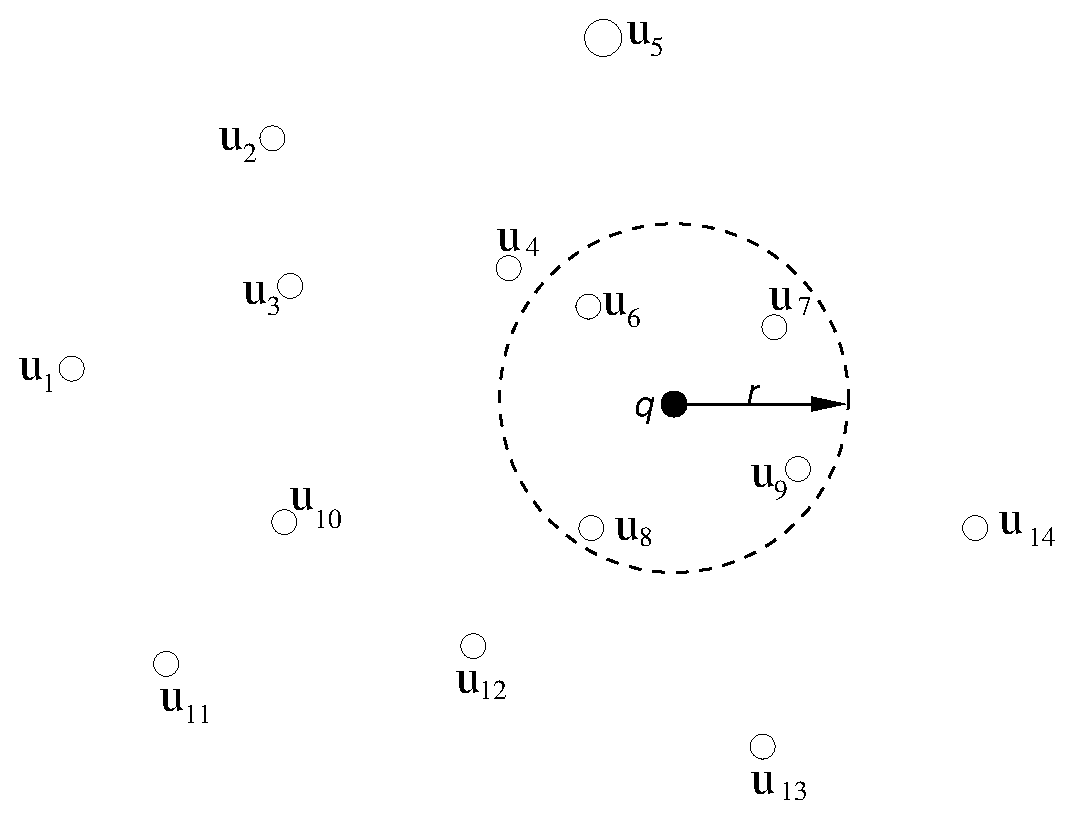
\psfig{file=imagenes/query-rangoL2.eps,width=70mm} &
     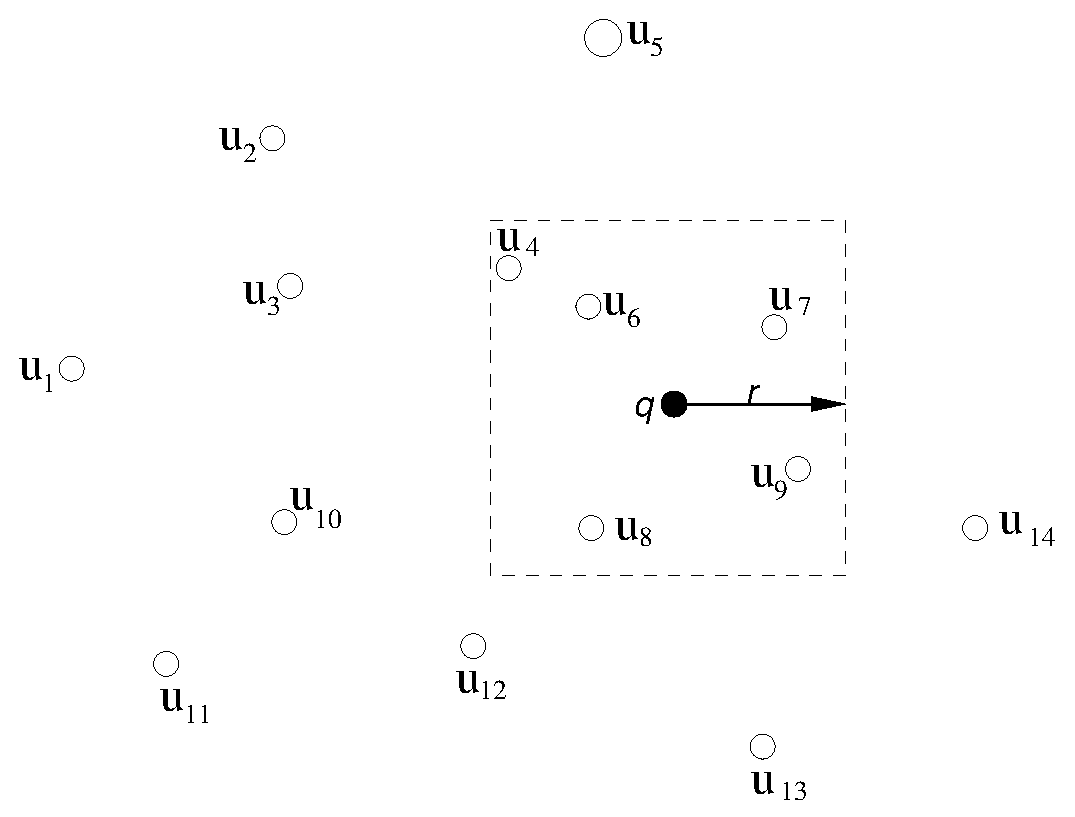
\psfig{file=imagenes/query-rangoLI.eps,width=70mm} \\ \hline
  \end{tabular}}
  \caption [Ejemplos de b\'usquedas por rango $(q,r)_d$ en   $\mathbb{R}^2$]
     {\textsl{\footnotesize { Ejemplos de b\'usquedas por
      rango $(q,r)_d$, con $d=L_2$ (izquierda) y $d=L_\infty$ (derecha). }}}
\label{query-rango}
\end{figure}


La Figura \ref{query-rango} ejemplifica b\'usquedas por rango $(q,r)_d$ sobre un conjunto de puntos en $\Re^2$, usando como funci\'on de distancia $L_2$ (izquierda) y $L_{\infty}$ (derecha), dos casos particulares de la distancia $L_p$. Las l\'ineas punteadas representan aquellos puntos que est\'an ex\'actamente a distancia $r$ de $q$, por lo tanto todos aquellos elementos que caen dentro de estas l\'ineas forman parte del resultado de la b\'usqueda. La distancia $L_2$, m\'as conocida como \textit{Distancia Euclidiana}, se corresponde con nuestra noci\'on de distancia espacial. Las b\'usquedas con distancia $L_{\infty}$ se corresponde con la b\'usqueda por rango cl\'asica, donde el rango es un hiper-rect\'angulo $k$ dimensional.\\

En el \'ambito de espacios vectoriales existen soluciones eficientes para b\'usquedas por similitud, como por ejemplo: $KD-tree$, $R-tree$, $Quad tree$ y $X-tree$ entre otras. Estas t\'ecnicas usan informaci\'on sobre coordenadas para clasificar y agrupar puntos en el espacio. Desafortunadamente, las t\'ecnicas existentes son afectadas por la dimensi\'on del espacio vectorial. Por lo tanto, la complejidad de b\'usqueda por rango depende exponencialmente de la dimensi\'on del espacio.\\
 
Los espacios vectoriales pueden presentar grandes diferencias entre su dimensi\'on representacional y su dimensi\'on intr\'inseca (es decir la dimensi\'on real en la que se pueden embeber los puntos manteniendo la distancia entre ellos). Por ejemplo, un plano embebido en un espacio de dimensi\'on 50, tiene una dimensi\'on representacional de 50 y una dimensi\'on intr\'inseca de 2.\\

Por esta raz\'on, muchas veces se recurre a espacios m\'etricos generales, aun sabiendo que el problema de b\'usqueda es m\'as dif\'icil. No se debe descartar que tambi\'en es posible tratar un espacio vectorial como un espacio m\'etrico general usando solo la distancia entre los puntos. Una ventaja inmediata de esto es que toma peso la dimensi\'on intr\'inseca del espacio, independientemente de cualquier dimensi\'on representacional.\\

\section{Funciones de Distancia}

Cuando hablamos de funciones de distancia, podemos dividirlas en dos grupos, de acuerdo al tipo de valor que retornan:\\

\begin{itemize}
\item \textbf{Discretas}: son  aquellas que retornan un valor discreto como valor de distancia, como por ejemplo la distancia de edici\'on.
\item \textbf{Continuas}: son las que retornan un n\'umero real como distancia entreobjetos, como por ejemplo la distancia $L_2$ o distancia Euclidiana.
\end{itemize}

Describimos a continuaci\'on algunos ejemplos de funciones de distancia para espacios m\'etricos. \\

\noindent \textbf{\textit{Distancia de Minkowski}} \\

Como ya lo mencionamos, estas funciones forman realmente una familia de funciones denominadas m\'etricas $L_p$, ya que los casos individuales dependen del par\'ametro num\'erico $p$. Estas funciones se definen sobre vectores $K$-dimensionales de n\'umeros reales de la siguiente manera:

\[
L_p[(x_1,\ldots,x_K),(y_1,\ldots,y_K)] = \sqrt[p]{ \sum_{i=1}^k|x_i - y_i|^p}
\]

La m\'etrica $L_1$ es conocida como la distancia de Manhattan y la m\'etrica $L_2$ denota la distancia Euclidiana.\\

Para el caso de $p=\infty$, se toma el l\'imite de la f\'ormula anterior para $p$ tendiendo $\infty$. Se obtiene como resultado, que la distancia entre dos puntos del espacio vectorial es la m\'axima diferencia entre sus coordenadas:

\[
L_{\infty}((x_1,...,x_k), (y_1,...,y_k)) = max_{1 \leq i \leq k} |x_i - y_i |
\]

La funci\'on $L_{\infty}$ se conoce con el nombre de  distancia m\'axima, infinita o distancia de tablero de ajedrez.\\

Estas funciones son utilizadas en varios casos donde los vectores num\'ericos tienen condenadas independientes, por ejemplo, en mediciones de experimentos cient\'ificos, observaciones ambientales, o el estudio de diferentes aspectos de procesos de negocios.\\

\noindent \textbf{\textit{Distancia de  forma cuadr\'atica}}\\

En muchas aplicaciones que utilizan vectores de datos, los valores de las distintas dimensiones no son totalmente independientes. En estos casos las distancias de Minskowski no son aplicables ya que no tienen en cuenta la existencia de esta relaci\'on.\\

La distancia de forma cuadr\'atica  es utilizada en \'ambitos en los que existe una correlaci\'on entre  las dimensiones que componen el vector, ya que tiene el poder de modelar este tipo de  dependencias. La medida de distancia entre dos vectores $\bar{x}$ e $\bar{y}$  de $k$ dimensiones est\'a basada en una matriz positiva de pesos   $M_{k \times k}$ donde $m_{i,j}$  denotan cu\'an fuerte es la conexi\'on entre los componentes $i$ y $j$ de los vectores $\bar{x}$ e $\bar{y}$, respectivamente. Generalmente estos pesos son normalizados de manera que $0\leq m_{i,j} \leq 1$ donde las diagonales $m_{i,	i} = 1$. La distancia de forma  cuadr\'atica generalizada $d_M$ se define como:

\[
d_M(\bar{x},\bar{y}) = \sqrt{(\bar{x} - \bar{y})^T \cdot M \cdot (\bar{x} - \bar{y})}
\]

\noindent donde el super\'indice $T$ denota la transposici\'on de vectores.\\

El c\'alculo de \'esta distancia puede ser muy caro en t\'erminos computacionales, dependiendo de la dimensionalidad de los vectores.\\

Notar que $M$ es la matr\'iz identidad, esta distancia se transforma en la distancia euclidiana.\\

\noindent \textbf{\textit{Distancia de Edici\'on}}\\

La cercan\'ia entre secuencias de s\'imbolos (cadenas) puede medirse de manera efectiva a trav\'es de la distancia de Edici\'on, tambi\'en conocida como distancia de Levenshtein. La distancia entre dos cadenas $x=x_1...x_n$ e $y=y_1...y_n$ est\'a definida como el n\'umero m\'inimo de operaciones at\'omicas de edici\'on (inserci\'on, eliminaci\'on y reemplazo) necesarias para transformar la cadena $x$ en la cadena $y$. En t\'erminos formales, las operaciones de edici\'on se definen como sigue:

\begin{itemize}
\item \textbf{insert:} inserci\'on del caracter $c$ en la posici\'on $i$ de la cadena $x$, en s\'imbolos: 
  \[ins(x,i,c)=x_1 x_2 \ldots x_i\ c\ x_{i+1} \ldots x_n\]
\item  \textbf{delete}: eliminaci\'on del caracter $c$ en la posici\'on $i$ de la cadena $x$, en s\'imbolos:
  \[del(x,i)=x_1 x_2 \ldots x_{i-1} x_{i+1} \ldots x_n\]
\item \textbf{replace}: sustituci\'on de un caracter $c$ de la cadena $x$ en la posici\'on $i$ por un nuevo caracter $c'$, en s\'imbolos:
  \[repl(x,i,c)=x_1 x_2 \ldots x_{i-1}\ c' \ x_{i+1} \ldots x_n\]
\end{itemize}


La funci\'on de distancia de edici\'on generalizada asigna pesos (n\'umeros reales positivos) a cada operaci\'on at\'omica, por esto, la distancia entre las cadenas $x$ e $y$ es el m\'inimo valor de la suma de los pesos de las operaciones at\'omicas necesarias para transformar $x$ en $y$. Si los pesos asignados a cada operaci\'on difieren, la distancia de edici\'on no es sim\'etrica (violando la propiedad (b) del punto 2.1) y por lo tanto, no es una funci\'on m\'etrica.\\

A los fines del presente trabajo, a todas las operaciones se le asigna un peso equivalente de uno.\\

\noindent \textbf{\textit{Distancia de Edici\'on de \'arbol}}\\

Esta distancia es una bien conocida medida de proximidad entre \'arboles, en la cual se define la distancia entre dos estructuras de \'arboles como el costo m\'inimo necesario para convertir el \'arbol fuente en el \'arbol destino utilizando un conjunto predefinido de operaciones de edici\'on sobre \'arboles, tales como la inserci\'on y la eliminaci\'on de un nodo. El costo individual de estas operaciones de edici\'on puede ser constante para todo el \'arbol, o puede variar de acuerdo al nivel en el cual se lleva a cabo la operaci\'on. La raz\'on de esta variaci\'on es que el costo de la inserci\'on de un nodo cercano al nivel de la ra\'iz puede ser m\'as significativo que el costo de agregar un nodo hoja. Por supuesto, esto depende del dominio de aplicaci\'on.\\

Dado que los documentos XML generalmente se modelan como \'arboles etiquetados, esta distancia puede utilizarse tambi\'en para medir las diferencias estructurales entre dos documentos XML.\\

\noindent \textbf{\textit{Coeficiente de Jaccard}}\\

Si quisi\'eramos medir la distancia en un tipo diferente de datos, como lo son los conjuntos, podemos utilizar el denominado coeficiente de Jaccard. Asumiendo dos conjuntos $A$ y $B$, el coeficiente de Jaccard se define como:
\[
d(A,B) = 1 - \frac{|A \cap B|}{|A\cup B|}
\]
Esta funci\'on se basa simplemente en la raz\'on entre las cardinalidades de la intersecci\'on y la uni\'on de los conjuntos comparados. Como un ejemplo de una aplicaci\'on que trabaja con conjuntos, supongamos que tenemos un registro con usuarios y direcciones de sitios web que visit\'o cada uno. Para evaluar la similitud en el comportamiento de cada usuario, podemos utilizar el coeficiente de Jaccard.\\


\section{Algoritmos de Indexaci\'on}

Los algoritmos de indexaci\'on sirven para organizar la informaci\'on o universo de datos en estructuras de datos o \'indices. Este pre proceso de la base de datos tiene como objetivo reducir el n\'umero de c\'alculos al momento de resolver una b\'usqueda. Un dise\~no eficiente de los \textit{algoritmos de indexaci\'on}, junto con la desigualdad triangular, permite descartar   elementos evitando comparar la query con cada uno de los elementos de la base o universo de datos. As\'i, dada una query, primero se recorre el \'indice para determinar un subconjunto de elementos candidatos a ser parte de la respuesta y luego se examinan esos conjuntos en forma exhaustiva para obtener la respuesta definitiva.\\

\subsection{Un Modelo Unificado}

Todos los algoritmos de indexaci\'on particionan la base de datos $U$ en subconjuntos $U_I$. El \'indice permite identificar una lista de $U_i$ que potencialmente contiene elementos significativos para la consulta. Por consiguiente, la b\'usqueda se reduce a:

\begin{itemize}
\item Recorrer el \'indice para obtener los  candidatos. El costo de este proceso se denomina \textit{complejidad interna}

\item Examinar exhaustivamente estos candidatos  a fin de encontrar los elementos que realmente forman el resultado de la b\'usqueda. El costo de este proceso se denomina \textit{complejidad externa}. 

\end{itemize}

\begin{figure}[tb]
\centerline{%
  \begin{tabular}{c c c}
  \\
     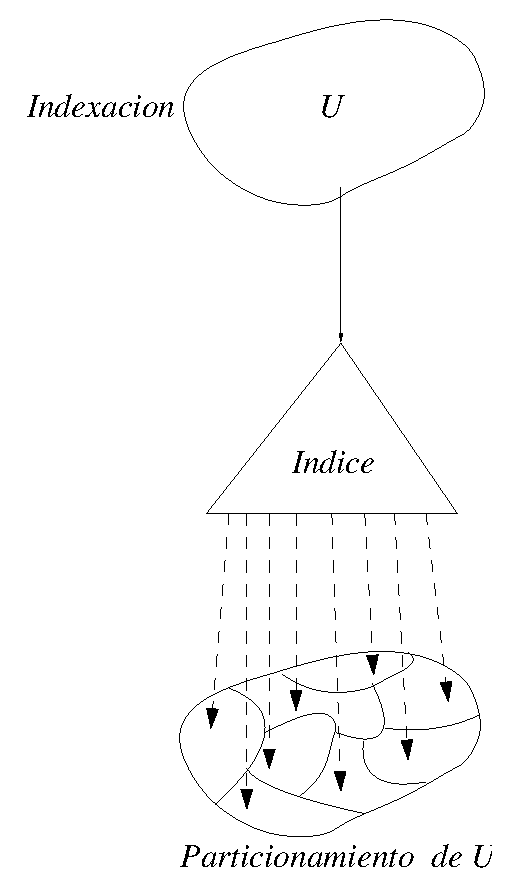
\psfig{file=imagenes/ejem-indice.eps,width=35mm} & \hspace{3cm}
     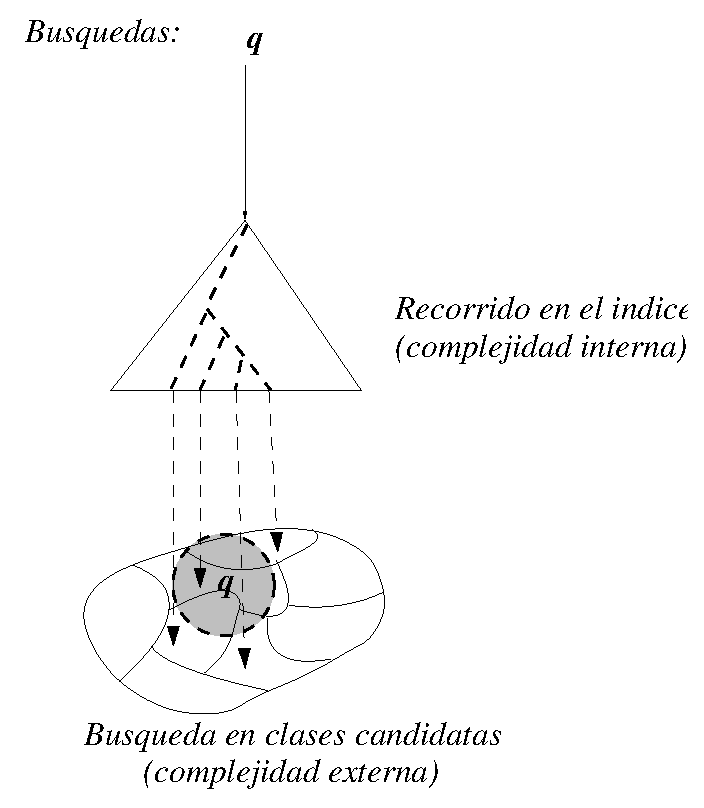
\psfig{file=imagenes/ejem-indice-bsq.eps,width=55mm}
  \end{tabular}}
  \caption[Modelo general de algoritmos de indizaci\'on]
  {\textsl{\footnotesize{ Modelo general de algoritmos de indexaci\'on para Espacios M\'etricos. }}}
\label{modelo-gral-indices}
\end{figure}

La Figura \ref{modelo-gral-indices} ejemplifica este modelo general de indexaci\'on. La figura de la izquierda muestra la divisi\'on en clases de equivalencia del espacio m\'etrico. La figura de la derecha muestra las clases de equivalencia que potencialmente contienen elementos relevantes para una b\'usqueda $q(r,d)$.\\

Para comprender totalmente el proceso de indexaci\'on se necesita entender adecuadamente los conceptos de relaci\'on de equivalencia y partici\'on de conjuntos. Aqu\'i, la relevancia de dichos conceptos se debe a la posibilidad de particionar un espacio m\'etrico en clases de equivalencias y obtener as\'i un nuevo espacio m\'etrico derivado del conjunto cociente.\\

Toda partici\'on $\pi(X) = \{\pi_1, \pi_2,...., \pi_n\}$ de un conjunto $X$ induce una relaci\'on de equivalencia (que denotamos con \textasciitilde ). Inversamente toda relaci\'on de equivalencia induce una partici\'on:

 \[
\forall x,y  \in X: x ~ y  \Leftrightarrow x \mbox{ est\'a en la misma parte que } y
\]


Las clases de equivalencia $[x]$ de esta relaci\'on se corresponden con las partes $\pi_i$ de la partici\'on $\pi$, es decir,

\[
\pi(X) = X/\textasciitilde
\]


Por consiguiente, los algoritmos de indexaci\'on existentes definen una relaci\'on de equivalencia sobre el espacio m\'etrico $X$. Las clases de equivalencia de $X$ en el conjunto cociente $\pi(X)$ pueden considerarse como elementos de un nuevo espacio m\'etrico, bajo alguna funci\'on de distancia $D: \pi(X)  \times \pi(X) \rightarrow  \Re^+$.\\

Ahora definimos la funci\'on $D_0$ que ser\'a de utilidad para encontrar la funci\'on $D$.

\[
D_0: 	\pi(X) \time \pi(X)  \rightarrow \Re^+
D_0([x],[y]): \min_{x \in [x], y \in [y]}\{d(x,y)\}
\]
			
$D_0$ representa la menor distancia entre un elemento de la clase $[x]$ y un elemento de la clase $[y]$. Esta distancia es el m\'aximo valor posible que mantiene el mapeo contractivo, es decir que $\forall x,y \in X : D_0([x],[y]) \leq d(x,y)$.\\
					
$D_0$ no puede ser utilizada con la finalidad de indexaci\'on porque no satisface la desigualdad triangular pero nos aproxima a una soluci\'on dado que sabemos que cualquier funci\'on de distancia $D$, que adem\'as cumple con las propiedades para ser una m\'etrica, es una cota inferior de $D_0$ (manteniendo as\'i el mapeo contractivo) que nos sirve para definir un nuevo espacio m\'etrico. En otras palabras, esta nueva funci\'on $D$ debe cumplir que $\forall [x],[y] en \pi(X),  D([x],[y]) \leq D_0([x],[y])$.\\

Luego, podemos convertir un problema de b\'usqueda en otro, que esperamos sea m\'as sencillo. Para una b\'usqueda $(q, r)_d$ primero, buscamos espacio $\pi(X, D)$ obteniendo como resultado $([q], r)_D = \{u \in  U/ D([u],[q]) \leq r\}$. Como $D_0$  es contractiva, podemos asegurar que $(q, r)_d \subseteq ([q], r)_D$.  Luego realizamos una b\'usqueda exhaustiva en $([q], r)_D$ a fin de determinar los elementos que forman parte de la respuesta a la consulta $(q, r)_d$.\\
				
Hay dos enfoques generales para crear estas relaciones de equivalencia: uno est\'a basado en pivotes y el otro se basa en particiones compactas o tipo Voronoi. Ambos se describen a continuaci\'on.

\subsection{Algoritmos Basados en Pivotes}

Los algoritmos de pivotes definen una relaci\'on de equivalencia basados en la distancia de los elementos a un conjunto de elementos preseleccionados que llamaremos \textit{pivotes}.\\

Sea $\{p_1, p_2,...,p_k\}$ un conjunto de pivotes, dos elementos son equivalentes si y s\'olo si est\'an a la misma distancia de todos los pivotes:

\[
x ~ p_i  y \Leftrightarrow d(x,p_i) = d(y,p_i) \forall_{i = 1....k}
\]

\begin{figure}[htb]
\centerline{ %
   \vspace{.2in}
   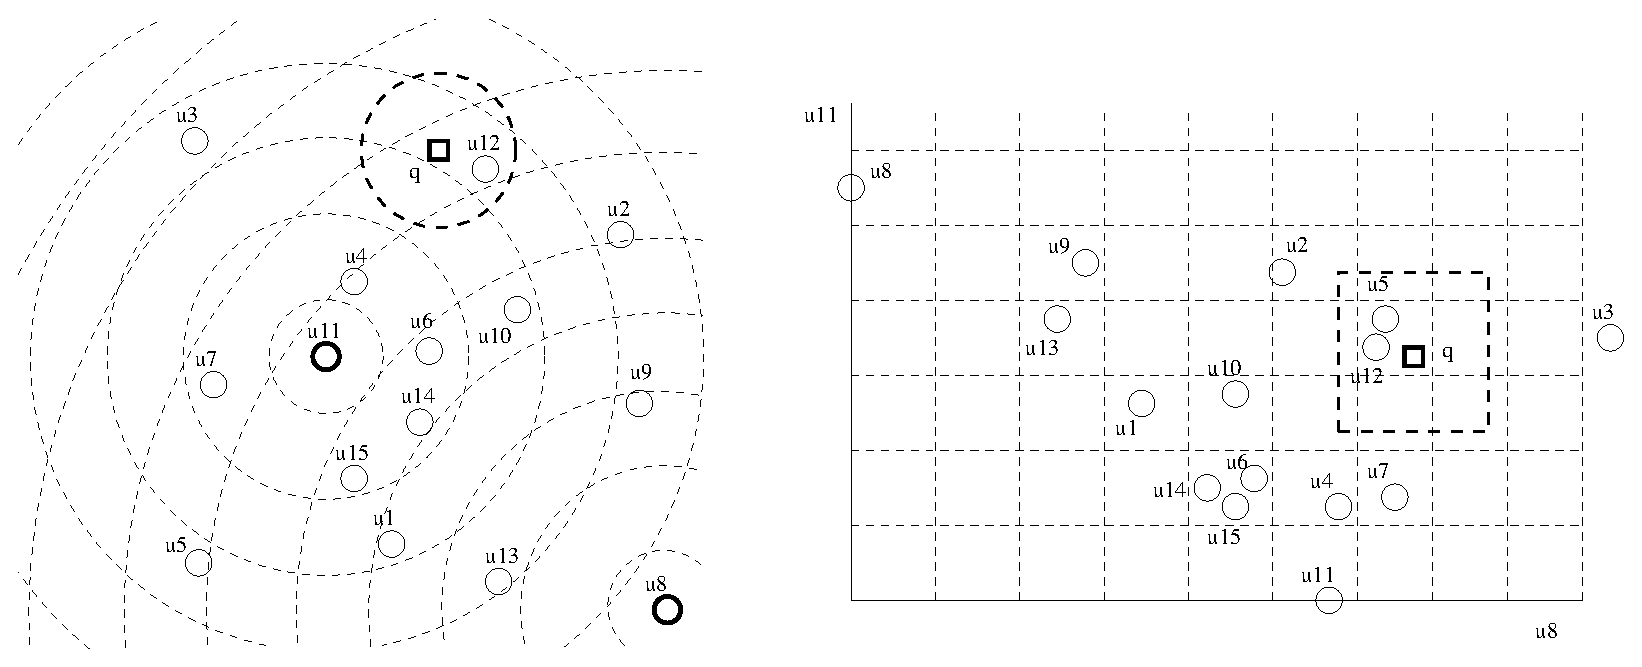
\psfig{file=imagenes/mapeo.eps, width=14cm}}
   \caption [Relaci\'on de equivalencia inducida por dos pivotes y su
   correspondiente transformaci\'on en un espacio vectorial]
     {\textsl{\footnotesize{Sobre la izquierda, un ejemplo de la relaci\'on de equivalencia inducida
        por la intersecci\'on de anillos centrados en dos pivotes, $u_8$ y $u_{11}$.
        Sobre la derecha se ilustra la transformaci\'on en un espacio vectorial de dimensi\'on 2.
    	Tambi\'en se grafica la transformaci\'on de una b\'usqueda $(q,r)_d$. }}}
\label{piv1}
\end{figure} 

Se puede ver que cada clase de equivalencia est\'a definida por la intersecci\'on de varias capas de esferas centradas en los puntos $p_i$ como se muestra en la Figura \ref{piv1}.\\

Veamos ahora cu\'al ser\'ia una funci\'on de distancia $D$ para las clases de equivalencia.  Por la desigualdad triangular, para cualquier $x \in X$, se cumple que:

\begin{itemize}
\item 1. $d(p,x) \leq d(p,y) + d(y,x) \Leftrightarrow d(p,x) - d(p,y) \leq d(y,x)$
\item 2. $d(p,y) \leq d(p,x) + d(x,y) \Leftrightarrow d(p,y) - d(p,x) \leq d(x,y)$
\item 3. $d(p,x) - d(p,y) \leq d(y,x) \wedge d(p,y) - d(p,x) \leq d(x,y) \Leftrightarrow |d(x,p) - d(y,p)| \leq d(x,y)$
\end{itemize}

Esto significa que, para cualquier elemento $p$ la distancia $d(x,y)$ no puede ser menor que $|d(x,p) - d(y,p)|$. Luego  $D([x],[y]) = |d(x,p) - d(y,p)|$  es un l\'imite inferior seguro para $D_0$. Si extendemos $D$ para $k$ los pivotes:

\[
D([x],[y]) = max_{1 \leq i \leq k} \{ |d(x,p_i) - d(y,p_i)|\} 
\]


Esta funci\'on de distancia $D$ limita inferiormente a $d$ y en consecuencia puede usarse como distancia en el espacio cociente.\\

La relaci\'on de equivalencia definida por un conjunto de $k$ pivotes tambi\'en puede considerarse como una proyecci\'on al espacio vectorial $\Re^k$. La i-\'esima coordenada de un elemento es la distancia al i-\'esimo pivote. Luego, a cada elemento $x$ del espacio le corresponde el vector  $\delta(x) = (d(x,p_1),d(x,p_2),...,d(x,p_k)) \in \Re^k$. Entonces, dada un consulta de b\'usqueda $(q,r)_d$ debemos encontrar un conjunto de elementos candidatos $([q],r)_D = x : D([q],[x]) \leq r$. En este caso particular significa encontrar los elementos tales que:

\[
max_{1 \leq i \leq k} \{ |d(x,p_i) - d(q,p_i)| \} = L_{\infty}(\delta(x),\delta(q)) \leq r 
\]


Esto significa que hemos proyectado el espacio m\'etrico original $(X, d)$ en el espacio vectorial $\Re^k$ con la funci\'on de distancia $L_{\infty}$. La Figura \ref{piv1}  ilustra estas ideas para un conjunto de puntos usando s\'olo dos pivotes.\\

\subsection{Algoritmos Basados en Particiones Compactas}

\begin{figure}[tb]
\centerline{%
\begin{minipage}{11cm}
\centerline{ %
   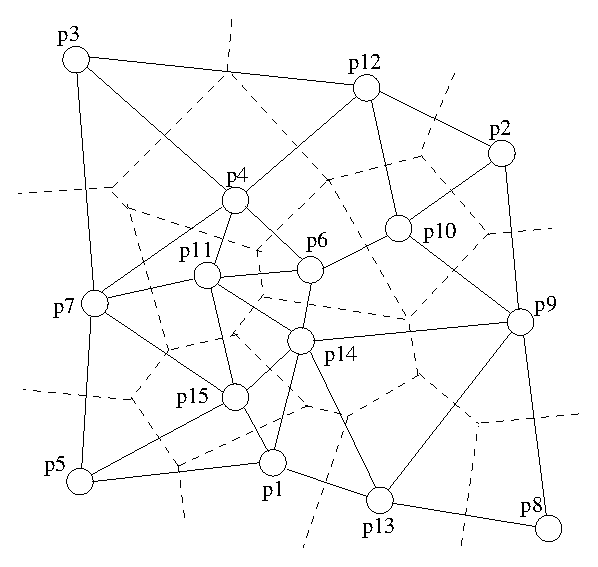
\psfig{file=imagenes/voronoi.eps, width=7cm} }
   \caption [Un ejemplo de Diagrama de Voronoi, y su concepto dual la Triangulaci\'on
      de Delanauy]
   {\textsl{\footnotesize{  Diagrama de Voronoi (l\'ineas punteadas)
     para  un  conjunto de puntos en $\mathbb{R}^2$ con distancia $L_2$; y su concepto
     dual la Triangulaci\'on de Delanauy.}}}
\label{vor-del}
\end{minipage}}
\end{figure}

La idea en este caso es dividir el espacio en particiones o zonas lo m\'as compactas posibles, almacenando puntos representativos de dichas zonas, denominados centros, y algunos datos extra que permitan descartar zonas completas lo m\'as r\'apidamente posible al momento de realizarse una consulta. Cada zona, a su vez, puede ser recursivamente particionada en m\'as zonas, lo cual induce una jerarqu\'ia de b\'usqueda.\\

\noindent \textbf{\textit{Criterio de partici\'on de Voronoi}}\\

Los Diagramas de Voronoi \cite{AUR91} han sido usados para b\'usquedas por proximidad en espacios vectoriales. Estos diagramas son una de las estructuras fundamentales dentro de la Geometr\'ia Computacional, de alguna forma ellos almacenan toda la informaci\'on referente a la proximidad entre puntos.\\

Se elige un conjunto de m centros ${c_1,c_2,...,c_m}$. El resto de los objetos se asignan a la zona de su centro m\'as cercano. Cuando todos los objetos de la base de datos son centros, el concepto de partici\'on de Voronoi descrito coincide con el concepto de dominio de Dirichlet [3]. La Figura \ref{vor-del} ejemplifica este concepto en un espacio vectorial 
de dimensi\'on 2.\\


Al momento de realizar una consulta $(q, r)_d$, se eval\'uan las distancias entre $q$ y los $m$ centros, eligiendo el centro m\'as cercano a $q$, el cual se denominar\'a $c$.\\

Si la bola de la consulta $(q, r)_d$ intersecta la zona de algun centro distinto a $c$, entonces se debe revisar exhaustivamente esa zona para ver si hay objetos que caigan dentro de la bola de consulta. Sea $x \in X$ un objeto perteneciente a la zona cuyo centro es $c_i$ y que se encuentra a distancia menor o igual que $r$ de la consulta $q$. Por la desigualdad triangular se tiene que:

\begin{enumerate}
\item [1.] $d(c,x) \leq d(c,q) + d(q,x) \leq d(c,q) + r$
\item [2.]$d(c_i,q) \leq d(c_i,x) + d(x,q) \leq d(c_i,x) + r  \Rightarrow d(c_i,q) - r \leq d(c_i,x)$
\end{enumerate}

Como $x$ pertenece a la zona de $c_i$ se cumple que  $d(c_i,x) \leq d(c,x)$. De esta condici\'on m\'as (1) y (2) se obtiene:

\begin{enumerate}
\item [3.] $d(c_i,q) - r \leq d(c_i,x) \leq d(c,x) \leq d(c,q) + r \Rightarrow d(c_i,q) - r \leq d(c,q) + r$
\end{enumerate}

Dada la condici\'on (3), se pueden descartar las zonas cuyo centro $c_i$ satisfaga la condici\'on $d(c_i,q)  > d(c,q) +2r$, dado que en ese caso dicha zona no puede tener intersecci\'on con la bola de consulta.

\section{Dimensi\'on en Espacios M\'etricos}

Uno de los grandes obst\'aculos en el dise\~no de algoritmos de b\'usqueda por similitud es la llamada maldici\'on de la dimensionalidad \cite{oursurvey}. Si se pudiera representar el conjunto de elementos de un espacio m\'etrico como puntos en un espacio vectorial, su dimensi\'on corresponder\'ia al n\'umero de coordenadas que tienen los puntos que lo componen. \\

Todos los algoritmos de b\'usqueda por similitud disminuyen su rendimiento cuando aumenta la  dimensi\'on del conjunto, hecho conocido como maldici\'on de la dimensionalidad. \\

En \cite{oursurvey} se muestra que el concepto de dimensi\'on de un espacio vectorial se puede extender a espacios m\'etricos generales utilizando el concepto de dimensi\'on intr\'inseca, y que la maldici\'on de la dimensionalidad tiene consecuencias similares en dichos espacios.\\

La distribuci\'on de distancias de un espacio m\'etrico se define como la probabilidad de que dos elementos se encuentren a cierta distancia $l$. Una aproximaci\'on a esta distribuci\'on es el \textit{histograma de distancias}, el cual se construye desde un subconjunto del espacio m\'etrico, calculando las distancias entre los elementos del subconjunto (ver figura \ref{defineH}).\\
 
 \begin{figure}[tb!]
\centerline{%
  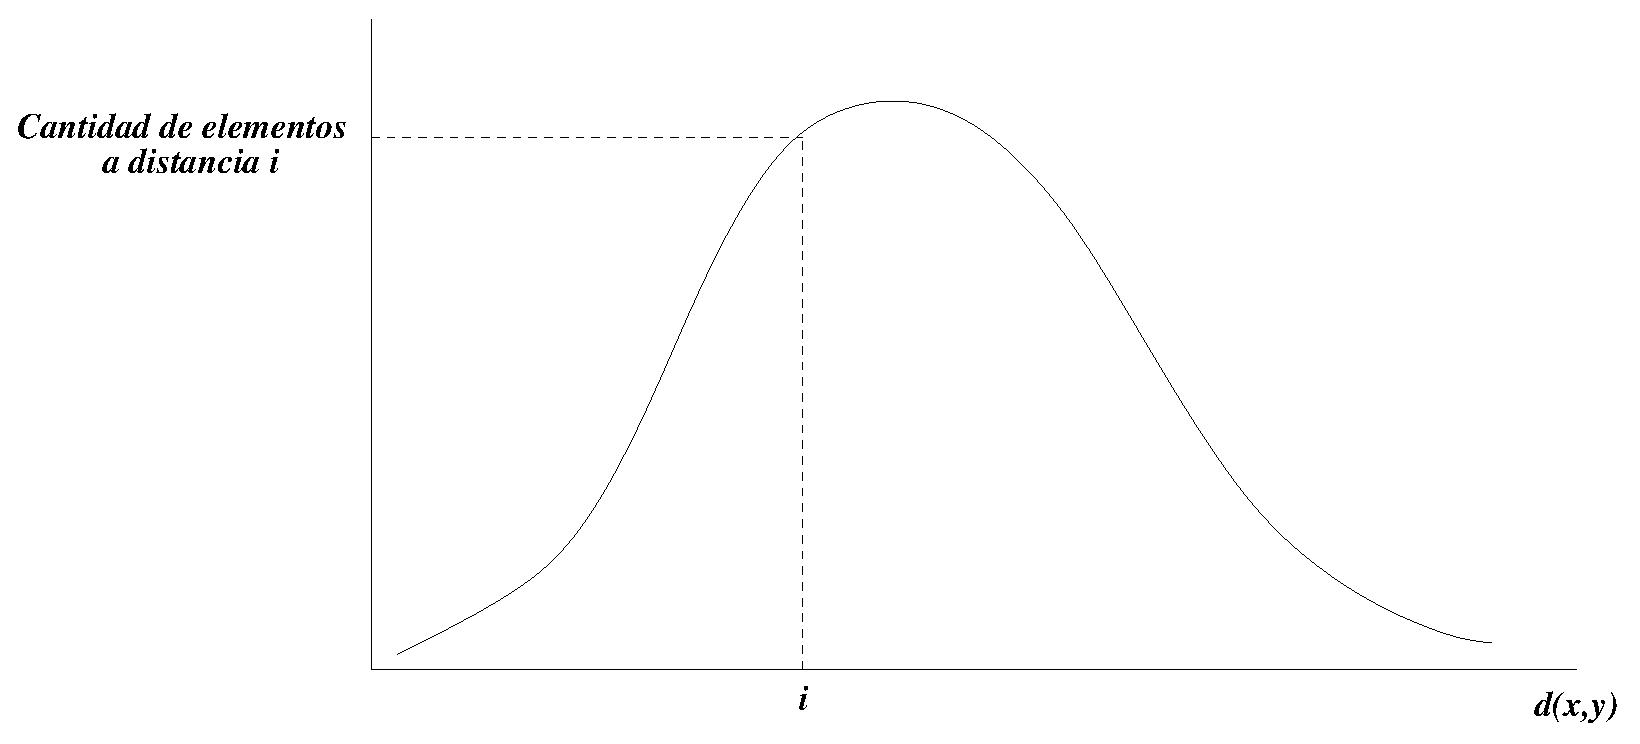
\psfig{file=imagenes/def-histo.eps,width=9cm}}
  \caption [Histograma de distancias de un espacio m\'etrico]
  {\footnotesize {\textsl {Histograma de distancias de un espacio m\'etrico}}}
\label{defineH}
\end{figure}

El histograma de distancias permite visualizar la distribuci\'on de los elementos del espacio m\'etrico y se menciona en varios art\'iculos como una medida fundamental relacionada a la dimensi\'on intr\'inseca del espacio \cite{Bri95, CM97, cn00,alenex,CPZ98a}. A medida que la dimensi\'on intr\'inseca de un espacio m\'etrico aumenta la media  $\mu$ del histograma crece y su varianza $\sigma^{2}$ se reduce.\\

\noindent En \cite{oursurvey} se define la dimensi\'on intr\'inseca de un espacio m\'etrico como:

\[
\gamma = \frac{\mu^2}{2\sigma^2}
\]

Los par\'ametros $\mu$ y $\sigma^2$ son la media y la varianza, respectivamente, del histograma de distancias de los puntos que conforman dicho espacio m\'etrico.\\

La figura \ref{dim1} da una idea intuitiva de por qu\'e el problema de b\'usqueda se torna m\'as dif\'icil cuando el histograma es m\'as concentrado.\\

Consideremos una b\'usqueda $(q,r)_{d}$ y un \'indice basado en pivotes elegidos aleatoriamente. En la figura se ejemplifican dos posibles casos para el histograma local respecto del punto $p$. Si $p$ es un pivote, estas gr\'aficas representan dos posibles distribuciones para los valores de $d(q,p)$. La regla de eliminaci\'on dice que podemos descartar aquellos puntos $y$ tales que  $y \notin [d(p,q)-r, d(p,q) + r]$. Las \'areas sombreadas muestran  los puntos que no podr\'an descartarse. Esto significa que a medida que el histograma se concentra m\'as alrededor de su media disminuye la cantidad de puntos que pueden descartarse usando como dato $d(p,q)$.\\

Este fen\'omeno es independiente de la naturaleza del espacio m\'etrico,  y nos brinda una forma de cuantificar cu\'an dif\'icil es una b\'usqueda sobre el mismo. Tal como se muestra experimental y anal\'iticamente en \cite{oursurvey}, todos los algoritmos degradan  sistem\'aticamente cuando la media $\rho$ del espacio se incrementa.\\

\begin{figure}[tb]
\centerline{%
  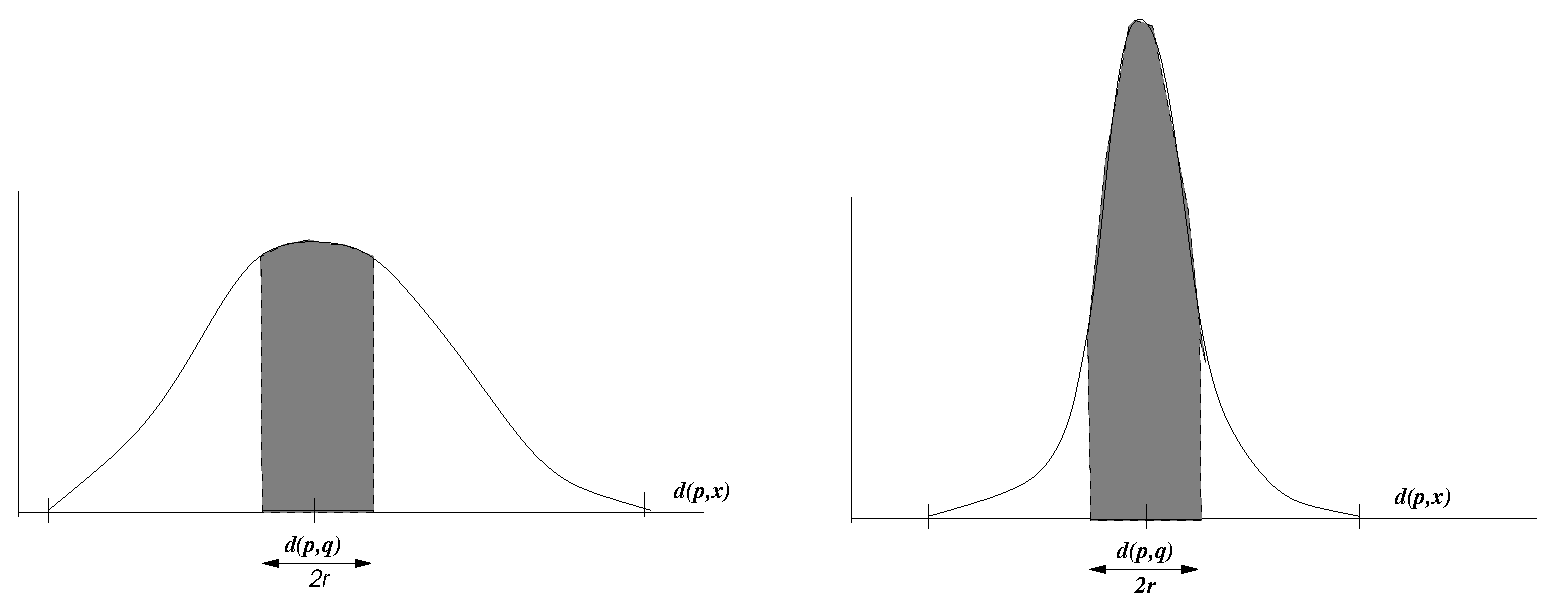
\psfig{file=imagenes/histog.eps,width=14cm}}
  \caption [Histogramas de distancias de baja y
             alta dimensionalidad]
    { \textsl{\footnotesize Histogramas de distancias de baja dimensionalidad
                (izquierda), y  de alta dimensionalidad (derecha)}}
\label{dim1}
\end{figure} 
\chapter{Enfoques computacionales a la calidad de informaci\'on en Wikipedia}

En el cap\'itulo anterior, se explicaron distintos aspectos relacionados a la calidad de la informaci\'on en Wikipedia. En este cap\'itulo abordaremos diferentes enfoques computacionales que capturan estos aspectos de calidad, los cuales podemos dividir en \emph{m\'etricas de calidad}, \emph{identificaci\'on de art\'iculos destacados}, \emph{detecci\'on de fallas en Wikipedia} y \emph{visualizaci\'on}. Cada uno de estos permite obtener, a trav\'es de diferentes formas y m\'etodos, indicadores que marcan si un art\'iculo de la Wikipedia en Ingl\'es contiene caracter\'isticas relacionadas a la calidad.

Como principal prop\'osito, en este cap\'itulo se mostrar\'an definiciones y ejemplos de cada uno de los enfoques, adem\'as, tambi\'en se presentar\'an caracter\'isticas y tareas puntuales para determinar aspectos de calidad en los art\'iculos de Wikipedia.

\emph{Organizaci\'on del cap\'itulo.} La subsecci\'on 3.1 presenta una definici\'on formal de \emph{m\'etricas de calidad} y se diferencia del concepto de \emph{medida}. Adem\'as se presentan diversas m\'etricas utilizadas en trabajos previos. La subsecci\'on 3.2, se enfoca en la tarea de identificar art\'iculos destacados y las caracter\'isticas que poseen para diferenciarlos del resto de los art\'iculos. La subsecci\'on 3.3 describe algunas fallas de calidad detectadas en los art\'iculos de Wikipedia y c\'omo los usuarios interact\'uan con las etiquetas de limpieza. La subsecci\'on 3.4 (falta definir).

\section{M\'etricas de calidad}

Actualmente, se ha puesto especial inter\'es en la definici\'on de m\'etricas de calidad sobre los art\'iculos de Wikipedia a trav\'es de diferentes criterios, marc\'andolo como un aspecto ampliamente importante dentro del \'area inform\'atica.

Hoy en día, se carece de una definici\'on formal de lo que una m\'etrica es, sin embargo, formularemos una definici\'on formal que se ajuste a lo que una m\'etrica es realmente.

En una primera instancia, definiremos y diferenciaremos los conceptos de \emph{medida} y \emph{m\'etrica}, los cuales podr\'ian parecer similares.

La estimaci\'on de la calidad de un art\'iculo de Wikipedia, se vincula directamente con la identificaci\'on y valoraci\'on de distintas \emph{propiedades} que este art\'iculo puede tener. En este contexto, en este trabajo diferenciaremos aquellas propiedades que son directamente \emph{medibles} de un art\'iculo de Wikipedia particular, que referenciaremos como \emph{medidas de calidad}, de aquellas que se definen en forma abstracta, como la \emph{combinaci\'on} de una o m\'as propiedades del art\'iculo y que llamaremos \emph{m\'etricas de calidad}. Por ejemplo, Stvilia ~\cite{StvTwSmGa:05} en su trabajo, define la \emph{completitud} como una m\'etrica de calidad que se calcula de la siguiente manera:


\begin{equation}
 \label{eq:ec1}
\begin{split}
& 0.4 \ \times \ Cantidad \ de \ v\acute{\imath}nculos \ internos \ rotos \ + \ 0.4 \ \times \ Cantidad \ interna \ de \\
& v\acute{\imath}nculos + \ 0.2 \ \times Longitud \ del \ art\acute{\imath}culo
\end{split}
\end{equation}

En este caso, la m\'etrica \emph{completitud} est\'a compuesta por las medidas: \emph{cantidad de v\'inculos internos rotos}, \emph{cantidad interna de v\'inculos} y \emph{longitud del art\'iculo}.

Las propiedades de un art\'iculo, tendr\'an asociadas un \emph{sistema de valoraci\'on} el cual, dado un documento, le hace corresponder el \emph{valor} (num\'erico) que dicho documento tiene para esta propiedad. M\'as formalmente, si $p$ es una propiedad cualquiera, su sistema de valoraci\'on $p^\sigma$ es una regla (o funci\'on) que asocia a cada art\'iculo de Wikipedia un valor num\'erico correspondiente con dicha propiedad $p$. Estas ideas son expresadas en notaci\'on matem\'atica en la siguiente definici\'on.
\\

\textbf{Definici\'on 1: Sistema de Valoraci\'on.} Sea $p$ una propiedad, $D$ el conjunto de art\'iculos de Wikipedia, y $N$ un valor de tipo num\'erico (por ejemplo el conjunto de los enteros ($\mathbb{Z}$) o el conjunto de los reales ($\realset$)). El \emph{sistema de valoraci\'on} $p^\sigma$ de la propiedad $p$, es una funci\'on: $$p^\sigma: D \rightarrow N$$

tal que para todo art\'iculo de Wikipedia $d \in D$, si $p^\sigma(d)=v$, $v$ representa el valor correspondiente a la propiedad $p$ en el art\'iculo $d$. Luego, diremos que ``$v$ es la \emph{valoraci\'on} de $d$ en la propiedad $p$'' o directamente que ``la propiedad $p$ de $d$ es $v$''. \label{def1}

Las propiedades m\'as sencillas de analizar son aquellas cuyos sistemas de valoraci\'on consisten en un \emph{instrumento} o \emph{m\'etodo} que obtienen el valor asociado con un documento directamente de una \emph{medici\'on} (\emph{aplicaci\'on}) directa del instrumento sobre el documento. En estos casos, los sistemas de valoraci\'on son en realidad \emph{sistemas de medici\'on} y a estas propiedades b\'asicas las denominaremos \emph{medidas de calidad}.

As\'i, por ejemplo, la \emph{longitud} de un art\'iculo, su \emph{riqueza de vocabulario}, el \emph{n\'umero de revisiones} que un art\'iculo ha tenido desde su revisi\'on, o la \emph{edad} del art\'iculo, son propiedades a las que se le puede asociar el valor correspondiente mediante la simple \emph{medici\'on directa} sobre el art\'iculo utilizando el instrumento (programa) adecuado que realiza el c\'alculo correspondiente. A modo de ejemplo, la biblioteca
NLTK\footnote{Biblioteca NLTK. www.nltk.org} (por Natural Language Toolkit) provee una colecci\'on interesante de programas en Python que implementan ese
tipo de instrumentos o medidas.

As\'i, por ejemplo, si $d$ es un art\'iculo arbitrario de Wikipedia, y $long$ representa la medida de calidad \emph{longitud} del
art\'iculo, $long^\sigma(d)$ representar\'a la longitud efectiva del art\'iculo $d$ (medido en bytes o palabras).

Adem\'as de estas propiedades b\'asicas, un art\'iculo puede tener otras propiedades m\'as abstractas, cuya definici\'on y valoraci\'on no
 son tan directas como en las medidas de calidad, y que en el contexto  de este trabajo llamaremos \emph{m\'etricas de calidad}.

Una m\'etrica de calidad, al igual que una medida de calidad, tambi\'en es una propiedad que permite asociar un valor num\'erico a un art\'iculo
de Wikipedia. Sin embargo, en este caso, la propiedad a ser cuantificada se define en base a otras propiedades del art\'iculo que
pueden estar dadas como medidas de calidad o m\'etricas de calidad. Es importante observar que mientras el valor de una propiedad
especificado por una medida es ``objetivo'', en el sentido que s\'olo depende de un instrumento de medici\'on apropiado de la caracter\'istica
a medir, las m\'etricas son ``estimaciones subjetivas'' ya que dependen de las propiedades particulares utilizadas en su definici\'on
y de la forma elegida para combinarlas.

Para ver m\'as claramente estas ideas, consideremos el caso de la m\'etrica  de calidad \emph{grado de informaci\'on}, que busca
capturar el grado de informaci\'on contenido en un art\'iculo. Esta caracter\'istica/m\'etrica es referenciada en Ingl\'es como la propiedad (abstracta) ``\emph{informativeness}''. Una primera aproximaci\'on para estimar la m\'etrica \emph{grado de informaci\'on}, podr\'ia consistir en basarla en la medida  \emph{longitud}, con el argumento de que a mayor longitud del art\'iculo, se supone que \'este contiene m\'as cantidad de informaci\'on. Un enfoque m\'as elaborado por otra parte, podr\'ia considerar que no s\'olo la informaci\'on textual es importante, sino que tambi\'en es muy \'util
considerar la medida de la \emph{cantidad de im\'agenes} que se muestran en el art\'iculo, tomando como lema la frase ``una imagen
vale m\'as que mil palabras''. En este ejemplo sencillo, es f\'acil observar que la decisi\'on de cu\'ales ser\'an las propiedades (medidas en
este caso) a utilizar y de la forma de ponderarlas y combinarlas, constituyen un aspecto \emph{subjetivo} y dependiente de la persona
encargada de definir la m\'etrica.

Una vez introducidas informalmente las similitudes y diferencias entre medidas y m\'etricas de calidad podemos decir, m\'as formalmente,
que una m\'etrica de calidad es una propiedad de un art\'iculo cuyo sistema de valoraci\'on se basa en otras propiedades de dicho
art\'iculo, las cuales a su vez pueden ser medidas o m\'etricas de calidad. Estas ideas son expresadas en notaci\'on matem\'atica en la
siguiente definici\'on.
\\

\textbf{Definici\'on 2: M\'etrica de calidad.} Sea $\mathcal{P}= \{p_1,p_2,\ldots,pn\}$ un conjunto de propiedades (medidas o m\'etricas de calidad) de un art\'iculo de Wikipedia y sean $D$ y $N$ los conjuntos introducidos en la Definici\'on 1.
Una \emph{m\'etrica de calidad} $\mu_\mathcal{P}$, definida en base a las propiedades en
 $\mathcal{P}$, es una propiedad cuyo sistema de valoraci\'on es una funci\'on: $$ \mu_\mathcal{P}^\sigma: D \rightarrow N$$ tal que para todo art\'iculo de
Wikipedia $d \in D$, si $\mu_\mathcal{P}^\sigma(d)= v$, $v$ representa el valor de la propiedad $\mu$ en el art\'iculo $d$, el
cual es computado en base a los valores $p_1^\sigma(d),p_2^\sigma(d),\ldots, p_n^\sigma(d)$, para todo $p_i \in \mathcal{P}$.

De la definici\'on anterior, es directo observar que la definici\'on de una m\'etrica de calidad, admite el uso de otras m\'etricas de calidad.
Por lo tanto, en estos casos, su valoraci\'on se resolver\'a en forma recursiva, hasta que la propiedad a valorar sea una medida de
calidad, cuyo valor se determina directamente por un sistema de medici\'on. En este sentido, es importante notar que la diferencia
antes mencionada entre \emph{medici\'on} (representada por una \emph{medida de calidad}) y \emph{evaluaci\'on estimativa}
(representada por una \emph{m\'etrica de calidad}) es similar a la que en Ingl\'es se realiza entre los t\'erminos \emph{measurement} y
\emph{assessment}.

Para clarificar los conceptos antes introducidos, continuemos con el ejemplo de la m\'etrica de calidad \emph{grado de informaci\'on} que representa el grado de informaci\'on (\emph{informativeness}) contenida en un art\'iculo de Wikipedia.

Si la m\'etrica \emph{grado de informaci\'on} (que abreviaremos $info$), es estimada como la suma de la \emph{longitud} del
art\'iculo (abreviada $long$) y el doble de la \emph{cantidad de im\'agenes} del art\'iculo (abreviada $cim$), es decir,

\begin{center}
\emph{grado de informaci\'on} $=$ \emph{longitud} $+$ $2$ $\times$
\emph{cantidad de im\'agenes}
\end{center}

la valoraci\'on del \emph{grado de informaci\'on} de un art\'iculo $d$ ($info^\sigma(d)$), se obtiene de la siguiente manera:

$$info^\sigma(d) = long^\sigma(d) + 2 \times cim^\sigma(d)$$

A modo de ejemplo, un art\'iculo de Wikipedia $d$ cuya longitud es de 126 palabras ($long^\sigma(d) = 126$), y que contiene 15 im\'agenes
($cim^\sigma(d) = 15$) tendr\'a un grado de informaci\'on estimado de 156 ($info^\sigma(d) = 156$)

Un ejemplo destacado, que plantea una mirada diferente, es el que podemos apreciar en las 7 m\'etricas de calidad aplicadas a art\'iculos de Wikipedia creadas por Stvilia ~\cite{StvTwSmGa:05}. Podemos ver como cada una de estas m\'etricas est\'a definida en base a una o varias medidas como se explic\'o anteriormente.
\begin{enumerate}
	\item \emph{Autoridad / Reputaci\'on} = 0.2 $\times$ Cantidad editores \'unicos + 0.2 $\times$ Cantidad Total de ediciones + 0.1 $\times$
Conectividad\footnote{Cantidad de art\'iculos conectados a un art\'iculo particular a trav\'es de editores frecuentes} + 0.3 $\times$ Cantidad de veces que se revirti\'o + 0.2 $\times$ Cantidad v\'inculos externos + 0.1 $\times$ Cantidad de ediciones de usuarios registrados + 0.2 $\times$ Cantidad de ediciones de usuarios an\'onimos.
	\item \emph{Completitud} = 0.4 $\times$ Cantidad de v\'inculos internos rotos + 0.4 $\times$ Cantidad interna de v\'inculos + 0.2 $\times$ Longitud del art\'iculo
	\item \emph{Complejidad} = Puntuaci\'on de legibilidad de Flesch\footnote{Prueba de legibilidad de Flesch. \\ https://es.wikipedia.org/wiki/Prueba\_de\_legibilidad\_de\_Flesch-Kincaid}
	\item \emph{Informatividad} = 0.6 $\times$ Informaci\'on de Ruido\footnote{1- (La cuantificaci\'on del t\'ermino / vector de token antes de stemizar y aplicar palabra de paro) / (longitud del documento antes de ser procesado)} - 0.6 $\times$ Diversidad\footnote{(Cantidad de editores \'unicos / Cantidad total de ediciones} + 0.3 $\times$ Cantidad de Im\'agenes
	\item \emph{Consistencia} = 0.6 $\times$ Ediciones compartidas por el administrador\footnote{Cantidad de ediciones del administrador /
Cantidad total de ediciones} + 0.5 $\times$ Edad
	\item \emph{Actualidad} = Actualidad\footnote{El tiempo entre la fecha de volcado y la fecha de la \'ultima actualizaci\'on del art\'iculo medido en d\'ias)}
	\item \emph{Volatilidad} = Tiempo medio de reversiones
\end{enumerate}

Las nombradas m\'etricas fueron calculadas en cada art\'iculo de Wikipedia sobre un total de 236 art\'iculos destacados y 834 art\'iculos aleatorios y luego agrupados y clasificados de acuerdo a las medidas previamente mencionadas.

Los resultados mostrados luego de la aplicaci\'on de las mismas, mostraron exitosamente que pueden distinguir art\'iculos destacados del resto de los art\'iculos.

Otro enfoque relacionado con las m\'etricas que presenta un planteamiento distinto, podemos verlo en el trabajo de ~\cite{InDuRoSe:12}, en el cual se construyen grafos capturando diferentes aspectos. En dicha investigación se plantean las siguientes m\'etricas:

\begin{enumerate}
	\item \emph{Coeficiente de agrupamiento}: representa el promedio de los coeficientes de agrupamientos de los nodos. Para un nodo particular \emph{i} se define de la siguiente manera:


\begin{equation}
\label{eq:ecej2}
	C{_i} = \frac {e{_i}} {[\frac {k{_i}(k{_i}-1)} {2}]}
\end{equation}

Donde e$_{i}$ es el n\'umero de v\'inculos entre vecinos de \emph{i}. \\
k$_{i}$ es el n\'umero de vecinos del nodo \emph{i}.\\
{k$_{i}$(k$_{i}$-1)} / {2} es el n\'umero de v\'inculos cuando los vecinos est\'an completamente conectados.

	\item \emph{Longitud de trayectoria media}: representa la media del n\'umero m\'inimo de aristas que tiene que ser atravesado para llegar a un nodo desde todos los nodos de la red. La longitud de trayectoria media para un nodo \emph{i} se define de la siguiente manera.

\begin{equation}
\label{eq:ecej2.1}
Pi = \sum_{k=1}^{n} \frac {m_{k}} {n}
\end{equation}

Donde m$_{k}$ representa el n\'umero m\'inimo de nodos que deben ser atravesados para alcanzar el nodo \emph{i} desde el nodo \emph{k} y \emph{n} es el n\'umero total de nodos en la red.

Esta m\'etrica mide el n\'umero promedio de intermediarios entre dos nodos cualquiera en la red buscando el camino m\'as corto. Cuanto menor sea el valor de esta m\'etrica de una red, m\'as cerca se encuentran los nodos, representando una red con pocos agujeros estructurales.
\end{enumerate}

Como resultado de la aplicaci\'on de estas m\'etricas, se confirma que los agujeros estructurales en los grafos generados est\'an directamente asociados con la calidad.

Otro trabajo de investigaci\'on, realizado por  ~\cite{AnLih:04}, muestra una manera diferente de plantear las m\'etricas. En su lugar, mide la calidad de los art\'iculos a trav\'es del concepto \emph{``reputaci\'on'}' definido por dos m\'etricas que mostraremos a continuaci\'on. En particular, estas s\'olo se calculan sobre metadatos y no sobre el contenido de los art\'iculos.

\begin{enumerate}
\item \emph{Rigor}:  este aspecto est\'a marcado por el n\'umero total de ediciones de un art\'iculo. Como premisa, se supone que un art\'iculo que tiene muchas ediciones posee un tratamiento mucho mayor y m\'as profundo.

\item \emph{Diversidad}: esta caracter\'istica est\'a determinada por n\'umero total de usuarios \'unicos que editaron un art\'iculo particular. En otras palabras, se intenta ver la cantidad de diferentes usuarios (an\'onimos o registrados) que se expresaron en el mismo art\'iculo.
\end{enumerate}

Otros trabajos han planteado diferentes enfoques a la hora de abordar el tema m\'etricas. Veamos a continuaci\'on como se trataron y estudiaron.

Un enfoque destacado es planteado por Stvilia ~\cite{StvTwSmGa:05} en el que define 7 m\'etricas: autoridad, completitud, complejidad, informatividad, consistencia, precisi\'on y volatilidad. Ellas pueden ser evaluadas autom\'aticamente y probadas sobre una muestra representativa de la Wikipedia en Ingl\'es.

A trav\'es del an\'alisis estad\'istico de caracter\'isticas de art\'iculos aleatorios y sus metadatos de los historiales de edici\'on, se crearon perfiles de 19 medidas de calidad. Dichos perfiles fueron evaluados por redundancia usando la t\'ecnica de an\'alisis de factor exploratorio ~\cite{JoWi:98}, luego se construyeron las 7 m\'etricas de calidad. Por \'ultimo, se evaluaron las mismas midiendo la habilidad de capturar la varianza  de la calidad de la informaci\'on de la colecci\'on de datos, a trav\'es de agrupamientos y clasificaci\'on de perfiles etiquetados de las m\'etricas de calidad de las caracter\'isticas y art\'iculos aleatorios.

Estas m\'etricas de la calidad de la informaci\'on deb\'ian, como objetivo principal, generar estimaciones que capturen una porci\'on importante de la varianza de un art\'iculo y al mismo tiempo evitar sesgos y redundancias.

Otro enfoque, considerado como el conjunto m\'as relevante de \emph{m\'etricas de calidad} para el contexto de Wikipedia, fue propuesto por ~\cite{ZhuGau:00}, en el cual, para medir la calidad de las p\'aginas Web definieron las siguientes m\'etricas.
\begin{itemize}
\item \emph{Actualidad:} medido como el tiempo de actualizaci\'on de una p\'agina (respecto a la fecha actual).
\item \emph{Radio de informaci\'on a ruido:} computado como la relaci\'on entre la longitud total de los items del \'indice por sobre el tama�\~no de la p\'agina.
\item \emph{Disponibilidad:} computada como la relaci\'on entre el n\'umero de v\'inculos rotos y la cantidad de v\'inculos en toda la p\'agina.
\item \emph{Cohesi\'on:} el grado en el cual el contenido de una p\'agina se centra en un tema. Esto fue alcanzado gracias al directorio ontol\'ogico Magellan.
\item \emph{Autoridad:} m\'etrica basada en la revisi\'on de la vida de Internet de Yahoo, asignando valores entre 2 y 4 y el valor 0 en el caso que no haya sido revisada.
\item \emph{Popularidad:} estimada por el n\'umero de p\'aginas Web que citan a una p\'agina Web particular. Las puntuaciones fueron obtenidas de el buscador Altavista.
\end{itemize}

En el enfoque presentado por ~\cite{InDuRoSe:12}, se utiliza el m\'etodo de an\'alisis de redes sociales  ~\cite{WaFa:94}, en el cual plantearon a Wikipedia como una red de conocimiento que surge del conjunto de relaciones e interacciones entre los art\'iculos y los usuarios ~\cite{StaRD:00, KakSor:02}. En primer lugar, definieron una red de usuarios, donde cada nodo denota un usuario y cada relaci\'on entre ellos representa un art\'iculo com\'un al que han contribuido. Tambi\'en, existe otro grafo que se llama ``red de art\'iculos'' donde cada nodo representa un art\'iculo y cada enlace entre ellos representa un contribuidor com\'un. Ambas redes, con estructuras totalmente diferentes, capturan diferentes aspectos de interacci\'on, colaboraci\'on de la informaci\'on en la primera nombrada e informaci\'on tem\'atica en la segunda.
Como resultado del an\'alisis, se revela que clusters de art\'iculos de alta calidad se encuentran agrupados en lugares con agujeros estructurales.

Otro enfoque, explicado también en párrafos anteriores, se muestra en ~\cite{DavGf:03, UzSp:05}, donde se utilizaron dos m\'etricas: \emph{coeficiente de agrupamiento} y \emph{longitud de trayectoria media} para identificar la estructura de la red y, m\'as espec\'ificamente, la presencia o ausencia de un agujero estructural. La primera nombrada es  el promedio de los coeficientes de clustering de los nodos (grado de agrupamiento en que los nodos tienden a agruparse), mientras que la segunda es la media del n\'umero m\'inimo de aristas que tiene que ser atravesado para llegar a \'el desde todos los nodos de la red.

En el trabajo presentado por ~\cite{AnLih:04}, e introducido como ejemplo anteriormente, se mide la ``reputaci\'on'' de los art\'iculos a trav\'es de dos m\'etricas bien definidas, \emph{rigor} y \emph{diversidad}. La primera representa el n\'umero total de ediciones de un art\'iculo, que supone que a mayor cantidad de ediciones se provee un tratamiento m\'as profundo del objeto de estudio, mientras que el segundo, el n\'umero total de usuarios \'unicos, marca la cantidad de ``voces'' diferentes en el tema. Estos valores s\'olo fueron obtenidos considerando metadatos de los art\'iculos en cuesti\'on, sin considerar el contenido de los mismos. Para calcularlos se defini\'o un conjunto de temas de enciclopedia, los cuales son considerados ejemplares exactos y completos, contra los cuales se compararon los resultados obtenidos. Dichos resultados indican que hay una relaci\'on entre la historia del ``borrador del art\'iculo'' y las noticias de la actualidad.

Por otra parte, con el fin de medir la calidad de la informaci\'on basado en informaci\'on factual, en ~\cite{LeVoErFeCaHoGrr:12}, un enfoque diferente, se proponen tres enfoques: (i) el uso de simples estad\'isticas acerca de los hechos obtenidos de un texto, (ii) explotaci\'on de la informaci\'on relacional contenida en los hechos, y (iii) explotaci\'on de las relaciones sem\'anticas como meronimia y hiperonimia. Posteriormente, se propusieron para el primer enfoque caracter\'isticas estad\'isticas muy sencillas sobre hechos con el fin de determinar la capacidad informativa de un documento. Estas caracter\'isticas, que en ~\cite{LeVoErFeCaHoGrr:12} son nombradas como caracter\'isticas basadas en la frecuencia de hechos, son el antecedente m\'as cercano y la base para la mayor\'ia de las propuestas presentadas en \'este trabajo. Dichas caracter\'isticas ser\'an descritas en las pr\'oximas secciones con el fin de hacer m\'as f\'acil la comprensi\'on del concepto  ``soporte factual externo''.

Las caracter\'isticas basadas en la frecuencia de hechos s\'olo requieren informaci\'on sobre el n\'umero de hechos obtenidos por un proceso de extracci\'on de informaci\'on a partir de un recurso textual. Por ejemplo, si \emph{t} es un recurso textual arbitrario (un p\'arrafo, un documento, un corpus), y $F_{t}$ es la colecci\'on de hechos extra\'idos de \emph{t} por un m\'etodo extractor de informaci\'on arbitrario IE, se calcula directamente la cantidad de hechos de \emph{t}, denotado $F_{c}$(\emph{t}). Este es simplemente definido como el n\'umero total de hechos obtenidos de \emph{t} por IE, $f_{c}$ (t) = |$F_{\emph{t}}$|. Obviamente, la cantidad de hechos depende directamente del tama\~no del recurso textual \emph{t}, por lo que generalmente se normaliza de acuerdo al tama\~no de \emph{t}. Esta cantidad es referenciada en ~\cite{LeVoErFeCaHoGrr:12}, como la densidad factual de \emph{t}, y denota $f_{d}$ (\emph{t}). En ese caso, si \emph{size(t)} es una medida destinada a cuantificar el tama\~no de \emph{t}\footnote{Por ejemplo, podr\'ia ser el n\'umero de palabras o frases en \emph{T} o la longitud en n\'umero de caracteres de \emph{t}.}, la densidad factual de \emph{t}, se define como $f_{d}$ (\emph{t}) = $f_{c}$ (\emph{t}) / \emph{size(t)}.

Como se detallar\'a mas adelante, los hechos de la colecci\'on $F_{\emph{t}}$  se pueden utilizar para calcular el soporte factual externo de \emph{t}, donde t corresponde a un art\'iculo de Wikipedia.

En relaci\'on al uso de la informaci\'on ``externa'' para evaluar la calidad de la informaci\'on de un documento, vale la pena mencionar el trabajo de ~\cite{JuGrLe:09} en el contexto de una tarea de ranking de credibilidad de un blog. All\'i, los enfoques para evaluar la credibilidad de los blogs se basan en una comparaci\'on directa contra un corpus validado de noticias referenciadas. No utilizan informaci\'on factual y el dominio es diferente al que dirigi\'o en el presente art\'iculo, pero pudimos ver algunas similitudes en la idea de utilizar recursos externos como ``soporte'' del contenido interno de los documentos.

Probablemente, uno de los enfoques m\'as relacionados con nuestra propuesta se present\'o en ~\cite{MaWa:10}. Su enfoque para medir soporte de documentos de texto se basa en el uso de hechos muy b\'asicos derivados de frases sustantivo-a-sustantivo de un documento. Estos hechos se comparan con los obtenidos a partir de la informaci\'on recuperada por un motor de b\'usqueda conocido (Bing).

\section{Identificaci\'on de art\'iculos destacados}

En Wikipedia existen distintas calificaciones para los art\'iculos de acuerdo a su calidad como art\'iculo enciclop\'edico. El concepto formalizado a trav\'es del nombre \emph{Art\'iculo Destacado} (Featured Article), desde ahora llamado FA, corresponde a los mejores art\'iculos que Wikipedia puede ofrecer, seg\'un lo determinado por los ``Wikipedians'', editores de Wikipedia.

El art\'iculo destacado es identificado en el sitio Web de Wikipedia a trav\'es del icono de una estrella de bronce en la esquina superior derecha como se mostr\'o en secciones anteriores. Adem\'as, si el art\'iculo, tambi\'en es destacado en otros idiomas, una estrella aparecer\'a seguido al v\'inculo del lenguaje en la lista \emph{''En otros idiomas''}, posicionada del lado izquierdo de la p\'agina Web.

A modo de ejemplo, el art\'iculo \emph{''United States Bicentennial coinage''} (Monedas del Bicentenario de Estados Unidos), plasmado en la figura ~\ref{fig:usbicoinage}, corresponde a un art\'iculo destacado. El mismo trata acerca de monedas emitidas entre los a\~nos 1975 y 1976 en conmemoraci\'on a la independencia estadounidense. En el extremo superior derecho se remarca en rojo la estrella de bronce que indica la m\'axima calidad del art\'iculo en Wikipedia.

\begin{figure}[here]
	\begin{center}
		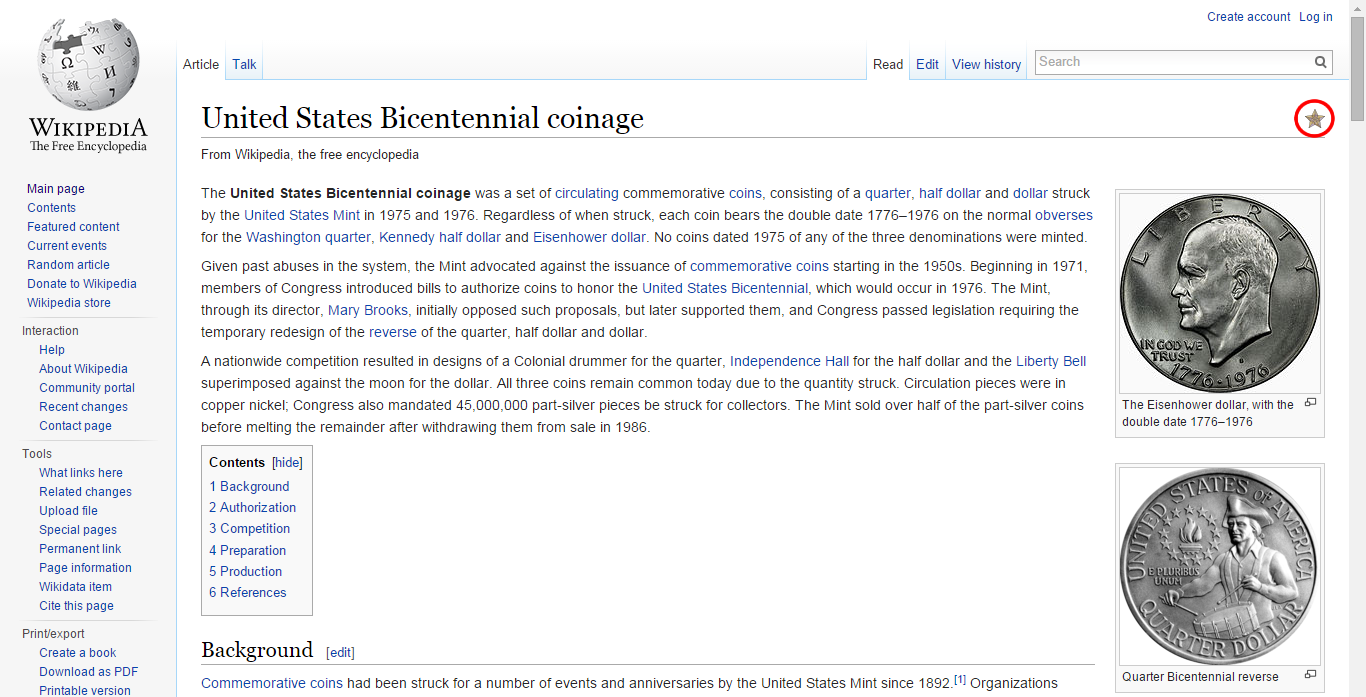
\includegraphics[width=1\textwidth]{imagenes/articulo_destacado1.png}
		\caption{Art\'iculo: United States Bicentennial Coinage (monedas del bicentenario de Estados Unidos). Extracto de un art\'iculo con la distinci\'on de art\'iculo destacado (se\~nalado con rojo). }
		\label{fig:usbicoinage}
	\end{center}
\end{figure}

Para clarificar lo nombrado en p\'arrafos anteriores acerca de art\'iculos destacados en otros idiomas, en la figura ~\ref{fig:estrellaamarilla}  podemos apreciar c\'omo un art\'iculo de la Wikipedia en Espa\~nol, nos indica a trav\'es de una estrella amarilla al lado de la palabra \emph{''English''}, que el mismo art\'iculo se encuentra en el idioma Ingl\'es y esa versi\'on corresponde a un art\'iculo destacado.

\begin{figure}[here]
	\begin{center}
		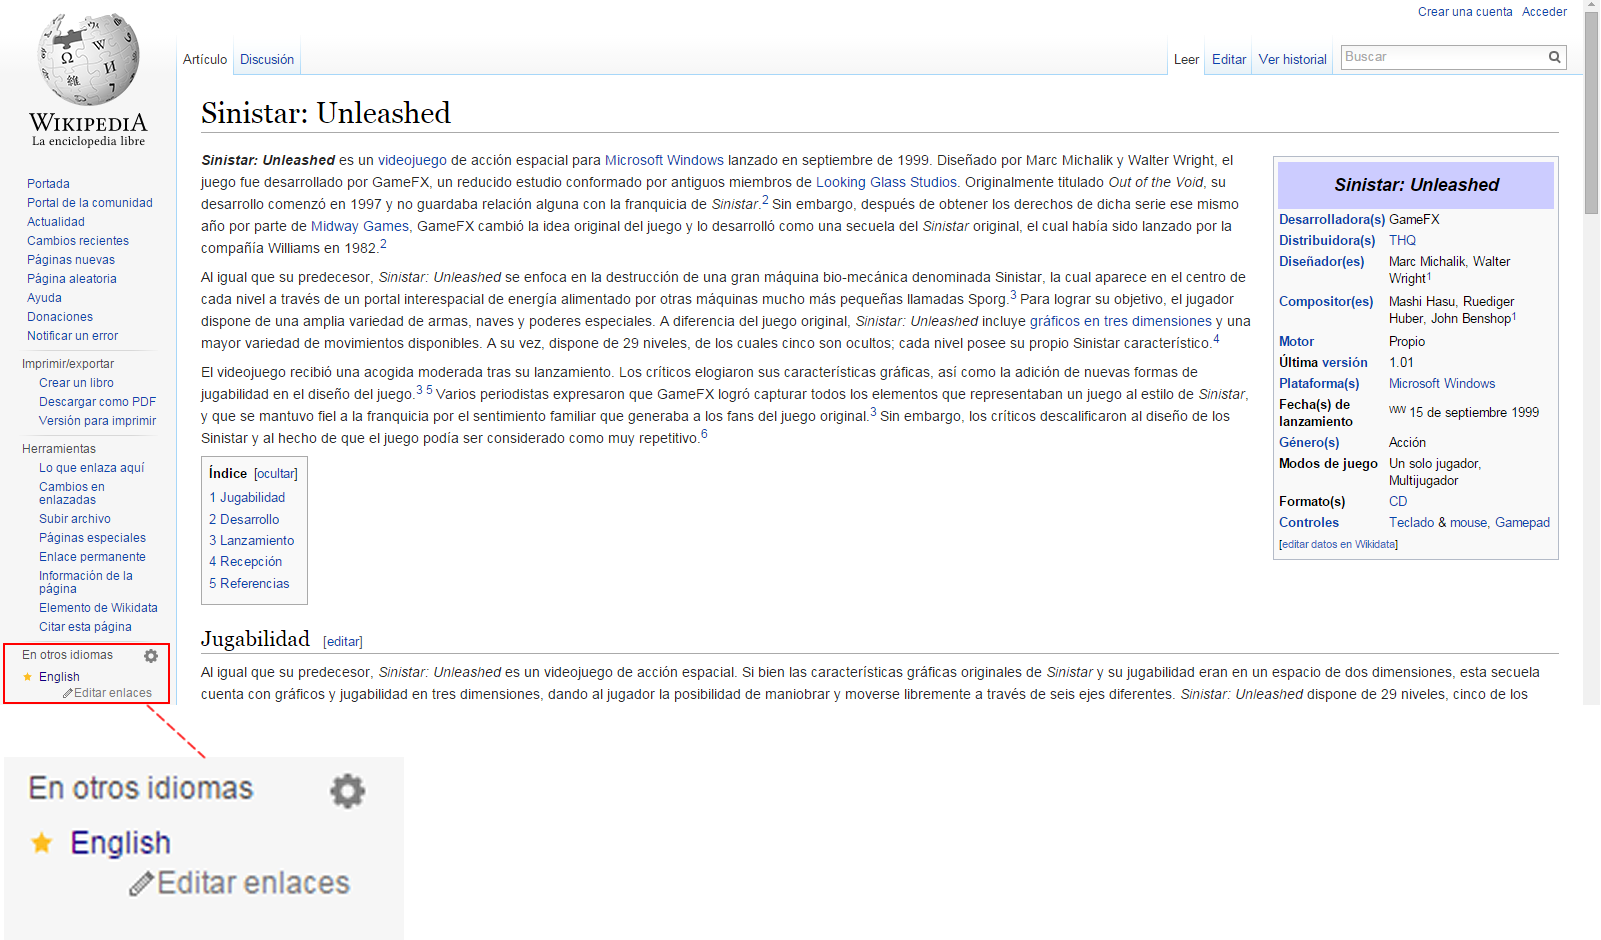
\includegraphics[width=1\textwidth]{imagenes/articulo_destacado3.png}
		\caption{Art\'iculo: Sinistar: Unleashed. Extracto de un art\'iculo con la distinci\'on de art\'iculo destacado (se\~nalado con rojo).}
		\label{fig:estrellaamarilla}
	\end{center}
\end{figure}

Actualmente, se cuenta con 4321 art\'iculos destacados en Ingl\'es de aproximadamente 3.454.284 . Esto indica que s\'olo el 0.1\% de los art\'iculos est\'a catalogado como FA.

Los criterios actuales que determinan un FA son: (1) completo; (2) preciso y verificable con fuentes; (3) estable; (4) bien escrito; (5) no controversial; (6) cumplir las normas de Wikipedia y gu\'ias de proyectos; (7) tener im\'agenes apropiadas; (8) tener longitud apropiada.

Profundicemos a continuaci\'on las caracter\'isticas nombradas aclaradas por Wikipedia\footnote{Criterios de Featured Articles. https://es.wikipedia.org/wiki/WP:QEUAD}.
\begin{itemize}
\item (1) Completo, implica que no omiten hechos, aspectos ni detalles importantes y que el art\'iculo tiene una extensi\'on adecuada sin perderse en detalles innecesarios, tratando con adecuada profundidad el tema.
\item (2) La informaci\'on debe ser precisa y verificable a trav\'es de referencias que muestre a quien se atribuye la sentencia. El art\'iculo debe estar basado en hechos y debe estar acompa\~nado de una lista de referencias que lo avalen.
\item (3) El art\'iculo no debe estar sometido a una guerra de ediciones constante ni modificar el contenido frecuentemente.
\item (4) El texto debe ser claro, conciso, convincente, sin faltas ortogr\'aficas, gramaticales o de estilo. El art\'iculo debe contener im\'agenes, tablas, gr\'aficos y otros elementos multimedia.
\item (5) El art\'iculo presentado, no debe contener citas que se contradigan o generen controversia. Los puntos de vista deben ser presentados sin sesgos y de manera justa.
\item (6) Debe cumplirse con el manual de estilo y seguir con la estructura formal de un art\'iculo, tales como un resumen conciso, tabla de contenidos, no contener v\'inculos a p\'aginas de desambiguaci\'on, etc.
\item (7) Las im\'agenes deben ser descriptivas y deben ser apropiadas,  intentando aclarar el contenido del art\'iculo.
\item (8) El art\'iculo no debe ser ni muy extenso ni muy corto, debe ser apropiado para expresar claramente la idea, con el nivel de detalle apropiado para el tema.
\end{itemize}

Un art\'iculo de Wikipedia debe someterse a un proceso para llegar a convertirse en FA. El mismo se convierte en destacado, luego de su nominaci\'on, revisi\'on y aprobaci\'on como art\'iculo candidato\footnote{Proceso de determinaci\'on de art\'iculos destacados \\ https://en.wikipedia.org/wiki/Wikipedia:Featured\_article\_candidates}. Los candidatos a art\'iculos destacados son revisados para determinar precisi\'on, neutralidad, integridad y estilo, de acuerdo a los criterios de los art\'iculos destacados nombrados anteriormente.

Aunque un art\'iculo destacado lleve tal distinci\'on, no significa que eventualmente pueda perderla. Esta situaci\'on puede darse por la introducci\'on de defectos debido a las diferentes ediciones que el art\'iculo sufra a lo largo del tiempo. Por este motivo, existe la Revalidaci\'on de Art\'iculos Destacados llamado RFA\footnote{Revalidaci\'on de Art\'iculos Destacados. \\ https://en.wikipedia.org/wiki/Wikipedia:Featured\_article\_review} (Review Featured Article), sistema por el cual permite acordar las correcciones que merece el art\'iculo.

Concentr\'emonos ahora en la tarea de diferenciar art\'iculos destacados de los que no lo son. La identificaci\'on de un art\'iculo destacado, es una tarea de clasificaci\'on binaria, que indica si el art\'iculo en cuesti\'on cumple o no las caracter\'isticas nombradas anteriormente. Definamos a continuaci\'on formalmente, en notaci\'on matem\'atica, a trav\'es de la siguiente funci\'on, la tarea de identificar art\'iculos destacados en Wikipedia.
\\

\textbf{Definici\'on 3: Identificaci\'on de un art\'iculo destacado.} Sea \emph{c} un clasificador, \emph{D} el conjunto de art\'iculos de Wikipedia, 0 y 1 valores enteros ($\mathbb{Z}$), la tarea de \emph{identificaci\'on de art\'iculos destacados}, es una funci\'on:

\begin{equation}
 \label{eq:ec1FFA}
\emph{c} :  \emph{D}  \rightarrow \emph{\{1,0\}}
\end{equation}

tal que \emph{c} es un clasificador que toma un art\'iculo de Wikipedia sobre el dominio \emph{D} y devuelve 1 en el caso de que el art\'iculo sea destacado o 0 en el caso que el art\'iculo no lo sea.

Luego de definir formalmente la tarea de identificaci\'on art\'iculos destacados y con el fin de seguir aclarando conceptos definidos en los p\'arrafos anteriores, veamos algunos ejemplos de este tipo de art\'iculos.

La figura ~\ref{fig:robinfriday} es un extracto de un art\'iculo destacado, acerca del futbolista profesional Ingl\'es Robin Friday nacido en el oeste de Londres, en el cual se muestra en el margen superior derecho, remarcado con un c\'irculo rojo, la estrella que indica que el mismo tiene el nivel de calidad m\'as alto en Wikipedia.

\begin{figure}[here]
	\begin{center}
		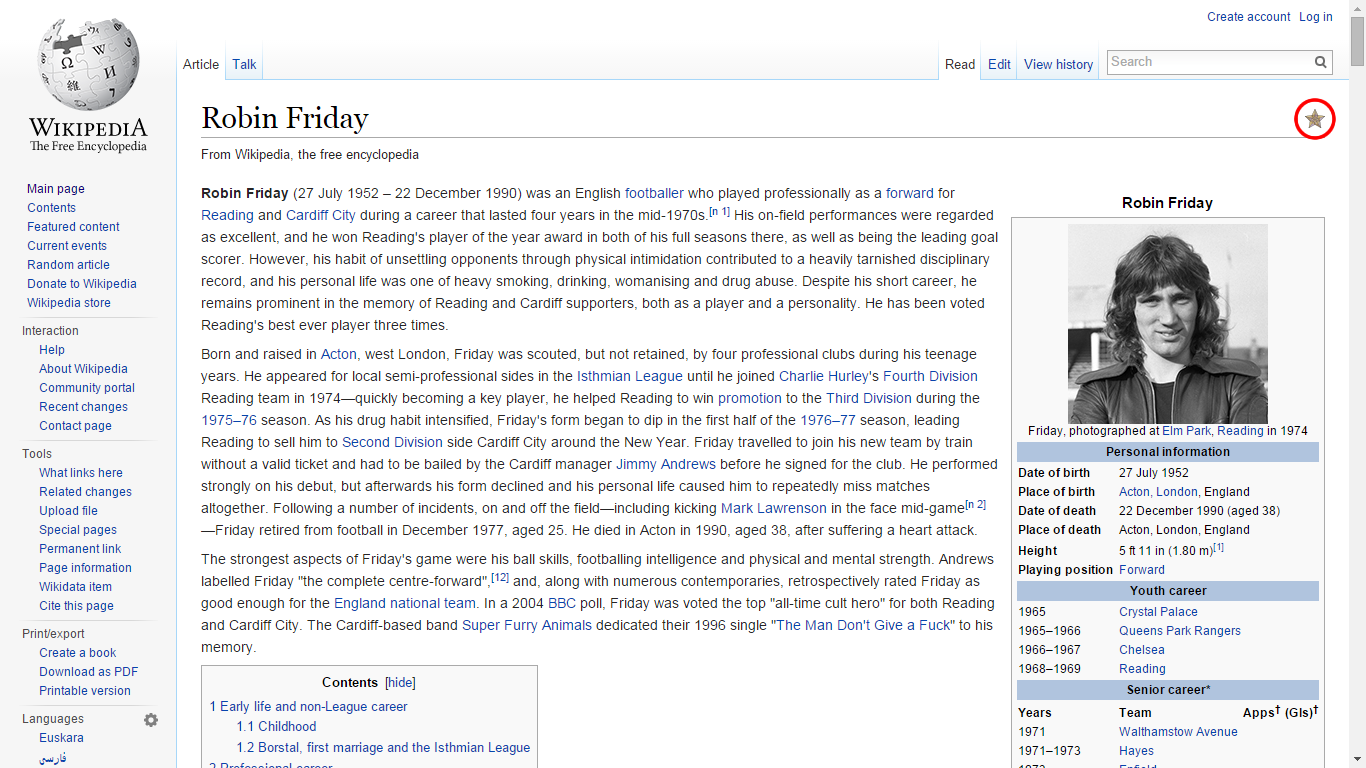
\includegraphics[width=1\textwidth]{imagenes/articulo_destacado.png}
		\caption{Art\'iculo: Robin Friday. Extracto de un art\'iculo con la distinci\'on de art\'iculo destacado (se\~nalado con rojo). }
		\label{fig:robinfriday}
	\end{center}
\end{figure}

Otro ejemplo de art\'iculo destacado, mostrado en la figura ~\ref{fig:sinistarunleashed}, podemos apreciarlo a trav\'es del art\'iculo \emph{Sinistar: unleashed}, correspondiente a un video juego de acci\'on de la empresa Microsoft presentado en el a\~no 1999. Tambi\'en, como se marc\'o en el ejemplo anterior, se indica con un c\'irculo rojo la estrella de bronce, categor\'ia de art\'iculo destacado para este art\'iculo de Wikipedia.

\begin{figure}[here]
	\begin{center}
		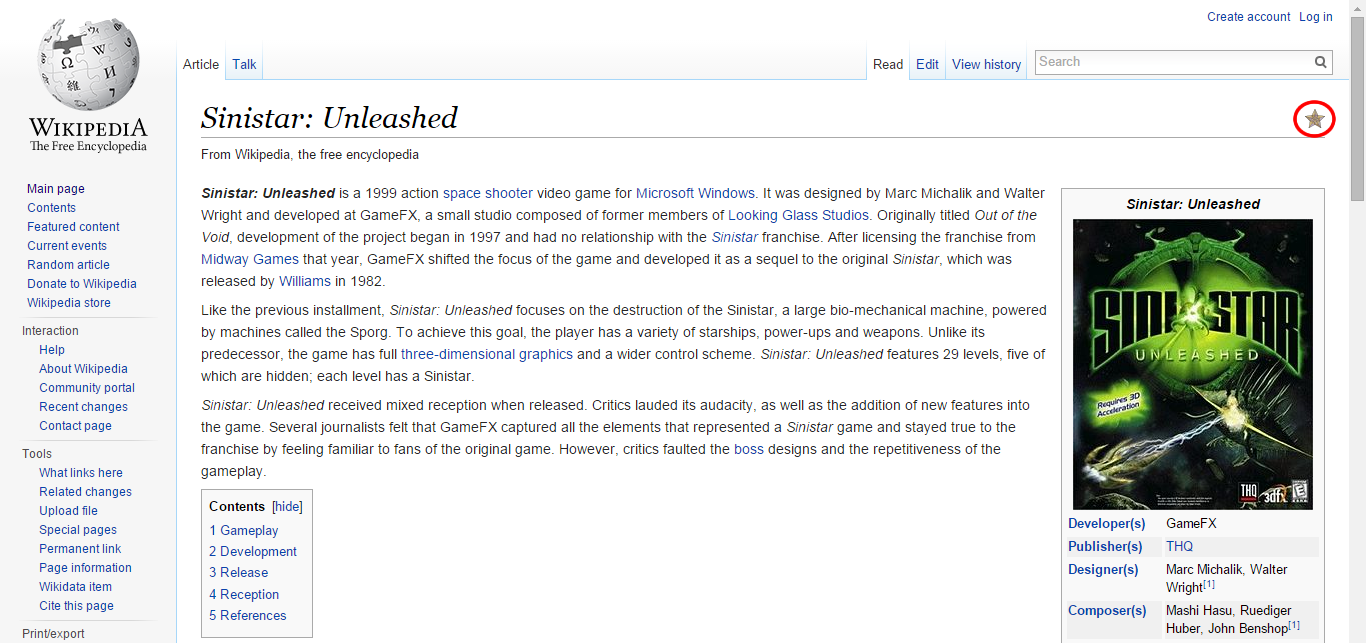
\includegraphics[width=1\textwidth]{imagenes/articulo_destacado2.png}
		\caption{Art\'iculo: Sinistar: Unleashed. Extracto de un art\'iculo con la distinci\'on de art\'iculo destacado (se\~nalado con rojo).}
		\label{fig:sinistarunleashed}
	\end{center}
\end{figure}

Wikipedia, afirma que provee una situaci\'on controlada respecto a la evaluaci\'on autom\'atica de la calidad de la informaci\'on, como fue se\~nalado en ~\cite{LiStei:10},  a trav\'es de la incorporaci\'on del concepto de art\'iculos destacados: “art\'iculos de alta calidad que son etiquetados de esa manera despu\'es de atravesar un extenso proceso de revisi\'on humana por pares” ~\cite{LiStei:10}. En pocas palabras, la comunidad de Wikipedia caracteriza como art\'iculos destacados aquellos que se distinguen por las normas profesionales de escritura, presentaci\'on, y el abastecimiento, los cuales se supone que poseen atributos espec\'ificos de calidad como bien escrito, amplio y bien investigado, neutral y estable como fue nombrado anteriormente.

En particular, la identificaci\'on autom\'atica de art\'iculos destacados (IFA) en Wikipedia es una tarea que ha ganado creciente inter\'es y ha sido abordada con diferentes enfoques. En el enfoque presentado por Blumenstock ~\cite{JoBl:08}, por ejemplo, sugiere utilizar simplemente el recuento de palabras como indicador de la calidad de los art\'iculos de Wikipedia. Sin embargo, en contraposici\'on, Lipka y Stein  ~\cite{LiStei:10} proponen otro m\'etodo sencillo y explotan la distribuci\'on de los trigramas de caracteres para identificar caracter\'isticas de alta calidad / buenos art\'iculos en Wikipedia.

Bas\'andonos en la interpretaci\'on de los metadatos, en el trabajo de ~\cite{WiHu:07} se presenta evidencia que los art\'iculos destacados pueden ser distinguidos de los no destacados a trav\'es del n\'umero de ediciones y editores, a mayor n\'umero de ediciones y editores,  mayor deber\'ia ser la calidad del art\'iculo.

Otra propuesta, que presenta una mirada desde un \'angulo similar, es el introducido por ~\cite{AnSmWi:09}, el cual no apunta a la medici\'on de los art\'iculos de Wikipedia, sin embargo, s\'i lo hace en la calidad de los contribuidores de Wikipedia. En este trabajo de investigaci\'on, detectaron que los usuarios registrados que hacen muchas contribuciones junto con contribuidores an\'onimos infrecuentes, generan contenido de alta calidad.

Como consecuencia del trabajo anterior, en ~\cite{LiRa:11}, se genera un aporte más importante, en el cual muestran c\'omo la calidad de Wikipedia no s\'olo depende de los diferentes tipos de contribuidores sino en c\'omo ellos colaboran entre s\'i.

Otros como ~\cite{WiHu:07} sostienen que la calidad de los art\'iculos est\'a estimada solamente con sus metadatos asociados sin requerir interpretaci\'on del contenido de los art\'iculos. Mientras que otros autores sostienen que cuando la identificaci\'on de art\'iculos destacados se realiza a trav\'es del an\'alisis del contenido, ~\cite{JoBl:08} es más apropiado realizar la medici\'on contando la cantidad de palabras en los art\'iculos.

Bas\'andose en el hecho de que los art\'iculos mas largos tienden a tener mas contenido factual, en un estudio propusieron la densidad factual ~\cite{LeVoErFeCaHoGrr:12}, con el fin de diferenciar art\'iculos destacados de art\'iculos que no lo son. Esta medida, relaciona la cantidad total de hechos del documento respecto a su longitud. Con este trabajo, se demostr\'o tambi\'en, que los art\'iculos destacados suelen ser m\'as informativos que los que no lo son, independientemente de su longitud ~\cite{PoFeErre:13}.

Por otro lado, otros trabajos presentaron enfoques diferentes y se basaron en simples estad\'isticas de los hechos obtenidos de los textos como la informaci\'on relacional contenida en los hechos y relaciones sem\'anticas como meronimia e hiperonimia entre otros ~\cite{LeVoErFeCaHoGrr:12}.

A pesar de la simplicidad (y eficacia) de los dos trabajos mencionados, en ~\cite{LeVoErFeCaHoGrr:12} se reconoce que para evaluar la precisi\'on factual del contenido de la Web, se requieren m\'as caracter\'isticas complejas sem\'anticas. Un enfoque com\'un es emplear extractores de informaci\'on abierta ~\cite{EtBaSoWe:12} o m\'etodos que utilizan conocimientos de fondo sobre relaciones sem\'anticas disponibles en recursos ontol\'ogicos como Wordnet ~\cite{Fel:98} y Yago ~\cite{StKaWe:07}. Estos enfoques extraen informaci\'on relacional acerca de las entidades nombradas en un texto particular (por ejemplo, hechos como f = (Mozart; naci\'o en; Salzburgo)). Adem\'as, se aprovechan las relaciones sem\'anticas definidas tales como meronimia e hiperonimia entre otras para inferir informaci\'on relacional entre entidades, que no se dan de forma expl\'icita en el texto.

A modo de aclaraci\'on y en contraposici\'on a los FA, el concepto de art\'iculo no destacado, desde ahora llamado NFA, representa un art\'iculo que no cumple con todas las caracter\'isticas de art\'iculo destacado (bien escrito, comprensivo, bien investigado, etc).

Vale destacar tambi\'en el concepto de un art\'iculo de Investigaci\'on Original (Original Research), desde ahora llamado OR, que surge de un documento que es una primera investigaci\'on, o est\'a escrito por los mismos investigadores que hicieron el estudio, con hip\'otesis o resultados reportados. Este conjunto de archivos corresponden a la colecci\'on de art\'iculos de investigaci\'on original del conjunto de entrenamiento suministrado en las competiciones PAN: Detecci\'on de Plagio, Autor Identificaci\'on, perfiles de autor\footnote{Competici\'on PAN. http://pan.webis.de/}. Esta colecci\'on cuenta con 506 archivos diferentes de Investigaci\'on Original y 939 de Art\'iculos no destacados.

\section{Detecci\'on de fallas en Wikipedia}

La detecci\'on de fallas de calidad en Wikipedia tiene como objetivo buscar imperfecciones de calidad espec\'ificas en los art\'iculos de la enciclopedia online. En otras palabras, las fallas, nos indican particularmente que una caracter\'istica del contenido debe ser modificada o agregada para mejorar su calidad y de esta manera no violar los est\'andares de calidad de Wikipedia.

\begin{table}
  \centering
   \begin{tabular}{ l l r }
	   \hline
	   & & \\
	   \textbf{Tipo de Falla} & \textbf{Descripci\'on de la Falla} & \textbf{Cantidad} \\ \\
	   \hline
     	   & & \\
	   Verificabilidad & Fuentes o referencias ausentes o & 98 \\
	   & inadecuadas  &  \\ \\
	   Estilo de escritura & No se ajusta al manual de estilo de & 74 \\
	   & Wikipedia  &  \\ \\
	   Miscel\'aneos & Fallas espec\'ificas, muy infrecuentes & 54 \\ \\
	   Temas espec\'ificos & Cuestiones que ocurren exclusivamente en & 44 \\
	   & ciertos temas &  \\ \\
	   Contenido no deseado & No se ajusta al criterio de inclusi\'on de & 42 \\
	   & Wikipedia &  \\ \\
	   Neutralidad & No escrito desde un punto de vista & 40 \\
	   & neutral &  \\ \\
	   Wiki tech & Cuestiones relacionadas a marcas, & 24 \\
	   & enlaces y categorizaci\'on &  \\ \\
	   Limpieza general & Problemas inespec\'ificos o generales & 17 \\ \\
	   Ampliar & Informaci\'on faltante o incompleta & 17 \\ \\
	   Estructura & Organizaci\'on inadecuada del contenido & 14 \\ \\
	   Sensibilidad al tiempo & Fuera de fecha o informaci\'on temporal no & 13 \\
	   & clara &  \\ \\
	   Unir & Contenido similar que debe ser combinado & 8 \\ \\
	  & & ---------- \\
 	  & & 445 \\
	\hline
 \end{tabular}
\caption {Los doce tipos de fallas generales con su respectiva descripci\'on y la cantidad de fallas de calidad que corresponden a ese tipo particular.}
\label{tablatfp1}
\end{table}

Para indicarles a los usuarios y editores de Wikipedia que un documento posee una falla de calidad en un art\'iculo o secci\'on, los usuarios de Wikipedia pueden optar por usar etiquetas de limpieza que se insertan dentro del documento llamadas \emph{cleanup tags}\footnote{Etiquetas de limpieza. https://en.wikipedia.org/wiki/Wikipedia:Cleanup}.

Las etiquetas pueden encontrarse en diferentes lugares del documento, ya que las fallas tienen como caracter\'istica que pueden tener diferentes alcances. Algunas fallas pueden referirse a todo el documento, por ejemplo indicando que \emph{faltan referencias} o simplemente a una secci\'on, indicando \emph{ampliar la secci\'on} o a\'un en otros casos, podemos encontrar reclamos particulares que indiquen, por ejemplo, que \emph{requiere una referencia} o que el \emph{v\'inculo se encuentra roto}. En el primero de los casos, encontramos la etiqueta al comienzo del documento de manera destacada, mientras que en el segundo se encuentra embebido en el texto.

Cabe destacar que en el snapshot correspondiente al 4 de enero de 2012 se identificaron 445 fallas de calidad en la Wikipedia en Ingl\'es  ~\cite{MaAn:13} y que las \emph{cleanup tags} son definidas por la comunidad de Wikipedia y pueden ser utilizadas por cualquier usuario.

La detecci\'on de dichas fallas de calidad, es usualmente considerada como un \emph{problema de clasificaci\'on de una clase}, donde para cada falla existente se construye un clasificador espec\'ifico para decidir si un art\'iculo de Wikipedia tiene dicha falla o no. A continuaci\'on definamos formalmente la falla de calidad en notaci\'on matem\'atica con el fin de clarificar los conceptos.\\

\textbf{Definici\'on 4: Detecci\'on de fallas de calidad.} Sea \emph{c} un clasificador, \emph{D} el conjunto de art\'iculos de Wikipedia, 0 y 1 valores enteros ($\mathbb{Z}$), la tarea de \emph{detecci\'on de fallas de calidad}, es una funci\'on:

\begin{equation}
 \label{eq:ec1FFC}
\emph{$c_{i}$} :  \emph{D}  \rightarrow \emph{\{1,0\}}
\end{equation}

tal que \emph{c} es un clasificador que toma un art\'iculo de Wikipedia sobre el dominio \emph{D} y devuelve 1 en el caso de que se identifique la falla \emph{i} en el art\'iculo o 0 en caso contrario.

Luego de definir formalmente la tarea de detecci\'on de fallas de calidad, a continuaci\'on veamos algunos ejemplos de fallas de calidad en Wikipedia que nos clarificar\'an los conceptos definidos anteriormente.

El art\'iculo de la Wikipedia en Ingl\'es que tiene como t\'itulo ``Murghazar''\footnote{Art\'iculo con fallas de calidad ``Murghazar''. https://en.wikipedia.org/wiki/Murghazar}, mostrado en la im\'agen ~\ref{fig:murghazar}, contiene diferentes fallas de calidad indicadas a trav\'es de etiquetas de limpieza. Al principio del documento, remarcado en rojo, encontramos una caja de etiquetas que nos indica que el documento tiene m\'ultiples cuestiones a corregir o mejorar. En primer lugar, el art\'iculo no cita fuentes o referencias. Adem\'as, el art\'iculo es hu\'erfano, lo que indica que no existen v\'inculos dentro de Wikipedia que lo enlacen. En \'ultimo lugar, se se\~nala que el art\'iculo esta escrito como si fuera publicidad. Tambi\'en, embebido en el texto, nos encontramos con etiquetas \emph{``[citation needed]''}, lo que nos indica que para esos fragmentos de texto, se necesitan citas que los avale.

\begin{figure}[here]
	\begin{center}
		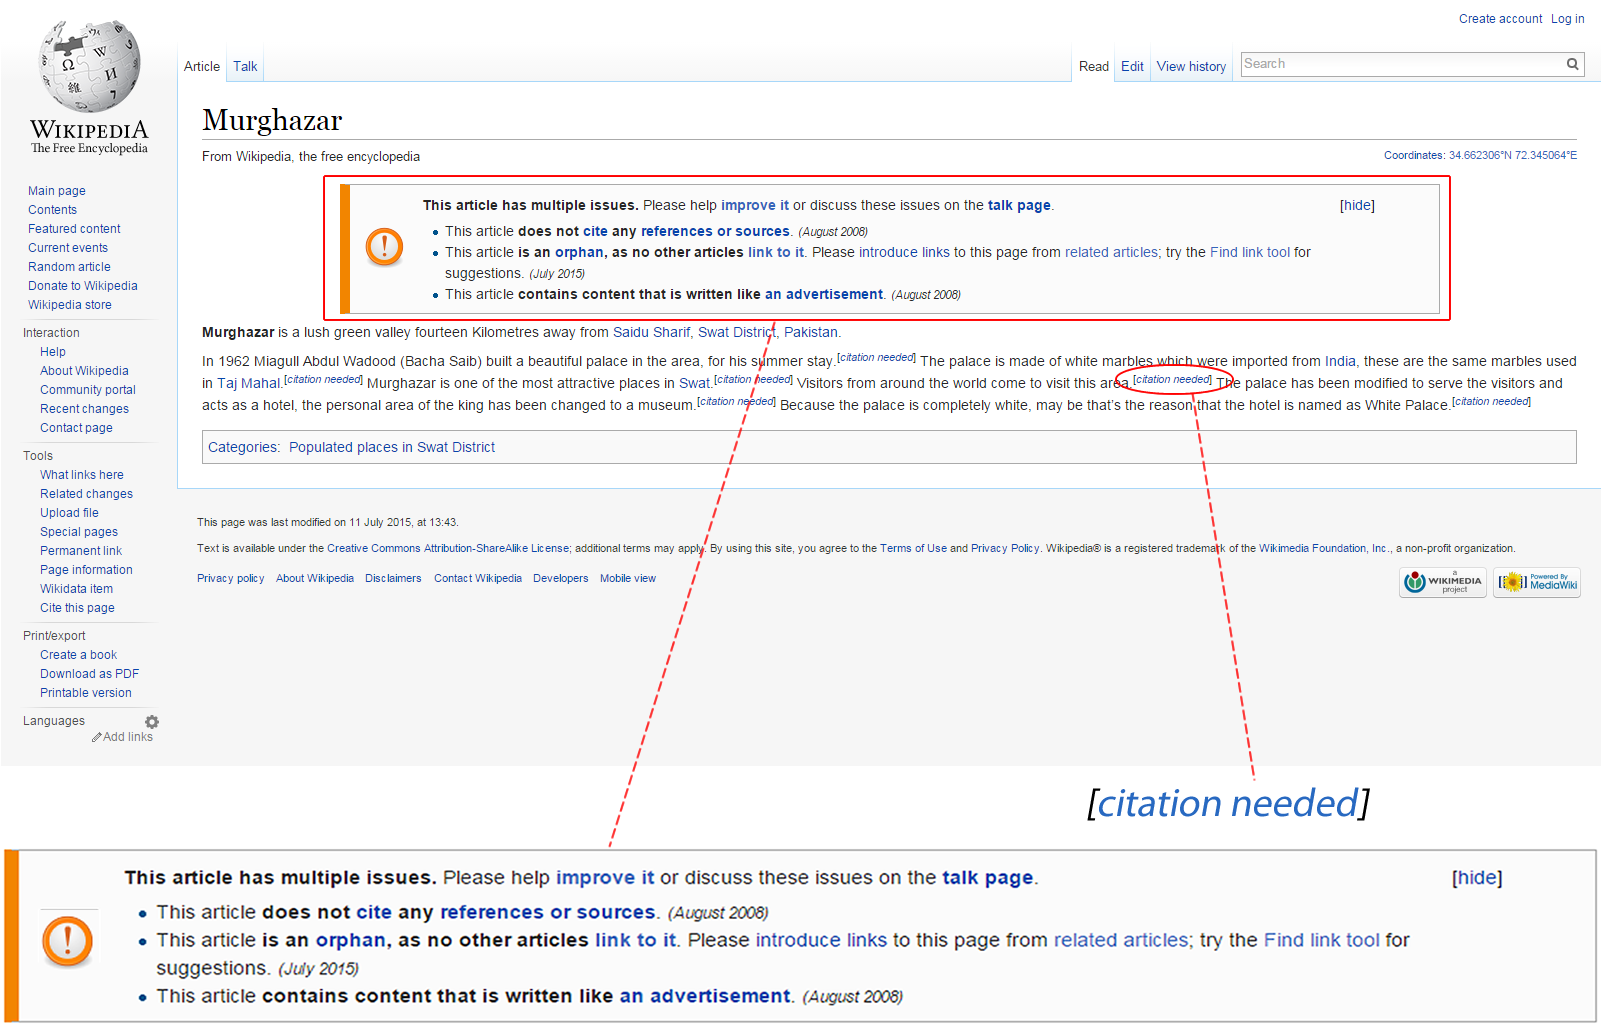
\includegraphics[width=1\textwidth]{imagenes/deteccion_falla.png}
		\caption{Art\'iculo de Wikipedia ''Murghazar'' con dos etiquetas de limpieza. La primera, ubicada al comienzo del art\'iculo indicando m\'ultiples cuestiones y la segunda, embebida en el texto indicando que faltan citas. }
		\label{fig:murghazar}
	\end{center}
\end{figure}

Otro ejemplo que muestra una falla diferente, podemos verlo en la figura ~\ref{fig:listgovernors}. Podemos apreciar el art\'iculo de la Wikipedia en Ingl\'es titulado ``List of Governors General of Canada''\footnote{Art\'iculo con fallas de calidad ``List of Governors General of Canada''. https://en.wikipedia.org/wiki/List\_of\_Governors\_General\_of\_Canada\#Governors\_ \\
General\_of\_the\_Province\_of\_Canada.2C\_1840.E2.80.931867} (lista de governadores generales de Canad\'a) en el cual se detectan falta de citas en ciertos fragmentos del texto indicandos\'e a trav\'es de la etiqueta \emph{``[citation needed]''}, y adem\'as, en el mismo art\'iculo, encontramos una caja de etiqueta en la secci\'on \emph{``Viceroys of Canada''} (\emph{``Virreyes de Canad\'a''}), que nos indica que esa secci\'on particular debe ser expandida o ampliada ya que se encuentra incompleta.

\begin{figure}[here]
	\begin{center}
		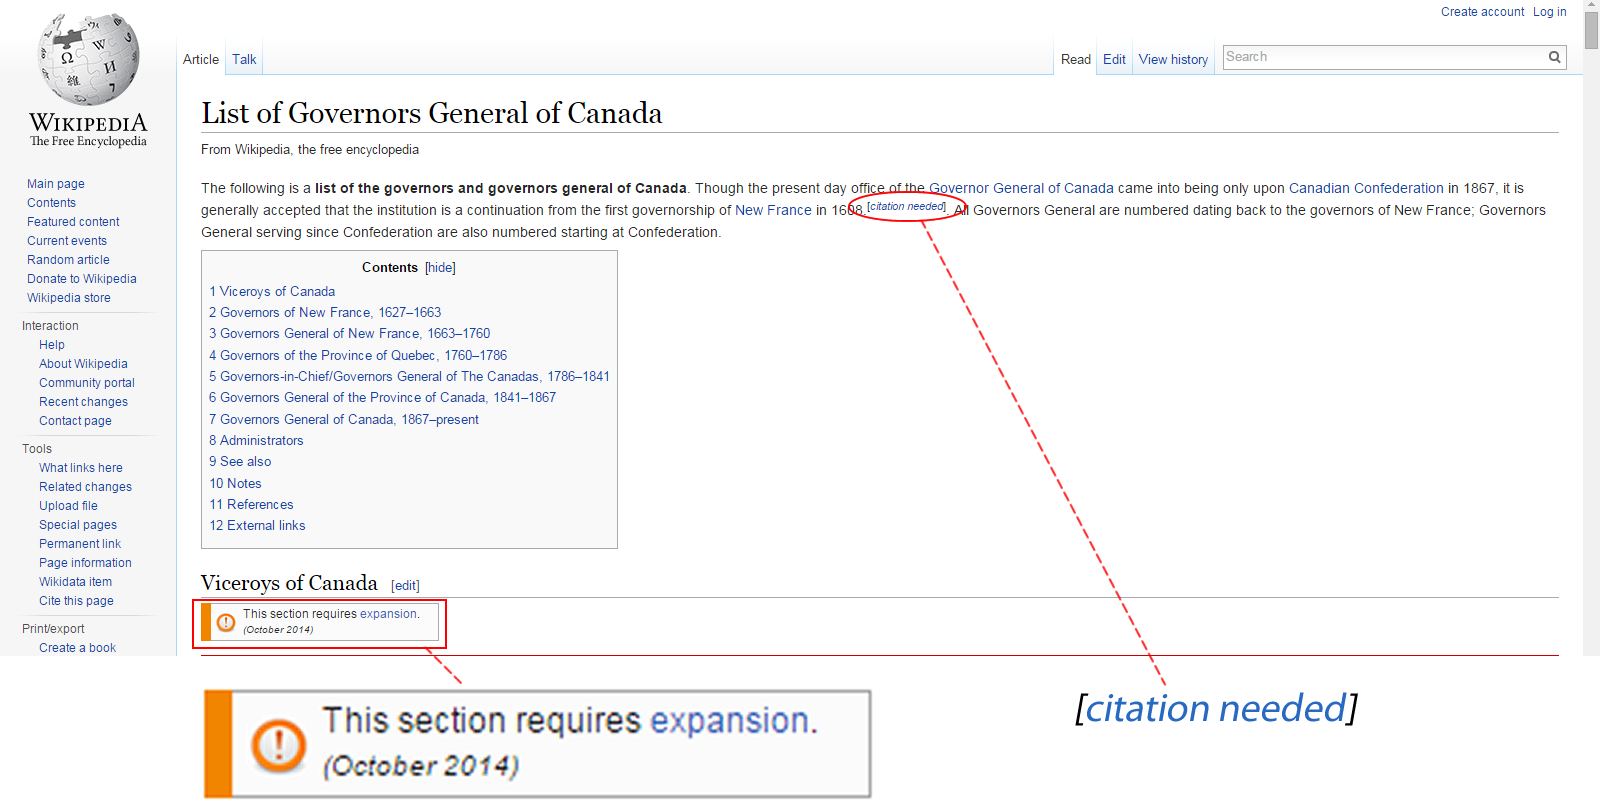
\includegraphics[width=1\textwidth]{imagenes/deteccion_falla2.png}
		\caption{Art\'iculo de Wikipedia ``List of Governors General of Canada'' con dos etiquetas de limpieza. Una indicando que una secci\'on debe ampliarse o mejorarse y otra embebida en el texto indicando que faltan citas. }
		\label{fig:listgovernors}
	\end{center}
\end{figure}

En la figura ~\ref{fig:hamptonwood}, como \'ultimo ejemplo, podemos apreciar el art\'iculo de la Wikipedia en Ingl\'es titulado ``Hampton Woods''\footnote{Art\'iculo con fallas de calidad ``Hampton Woods''.\\ https://en.wikipedia.org/wiki/Hampton\_Woods} en el cual al comienzo del art\'iculo se indica a trav\'es de una caja de etiquetas que posiblemente el art\'iculo contiene investigaci\'on original, ya que no existen fuentes que avalen la informaci\'on. Tambi\'en, inmediatamente debajo, se indica que no se citan referencias o fuentes.

\begin{figure}[here]
	\begin{center}
		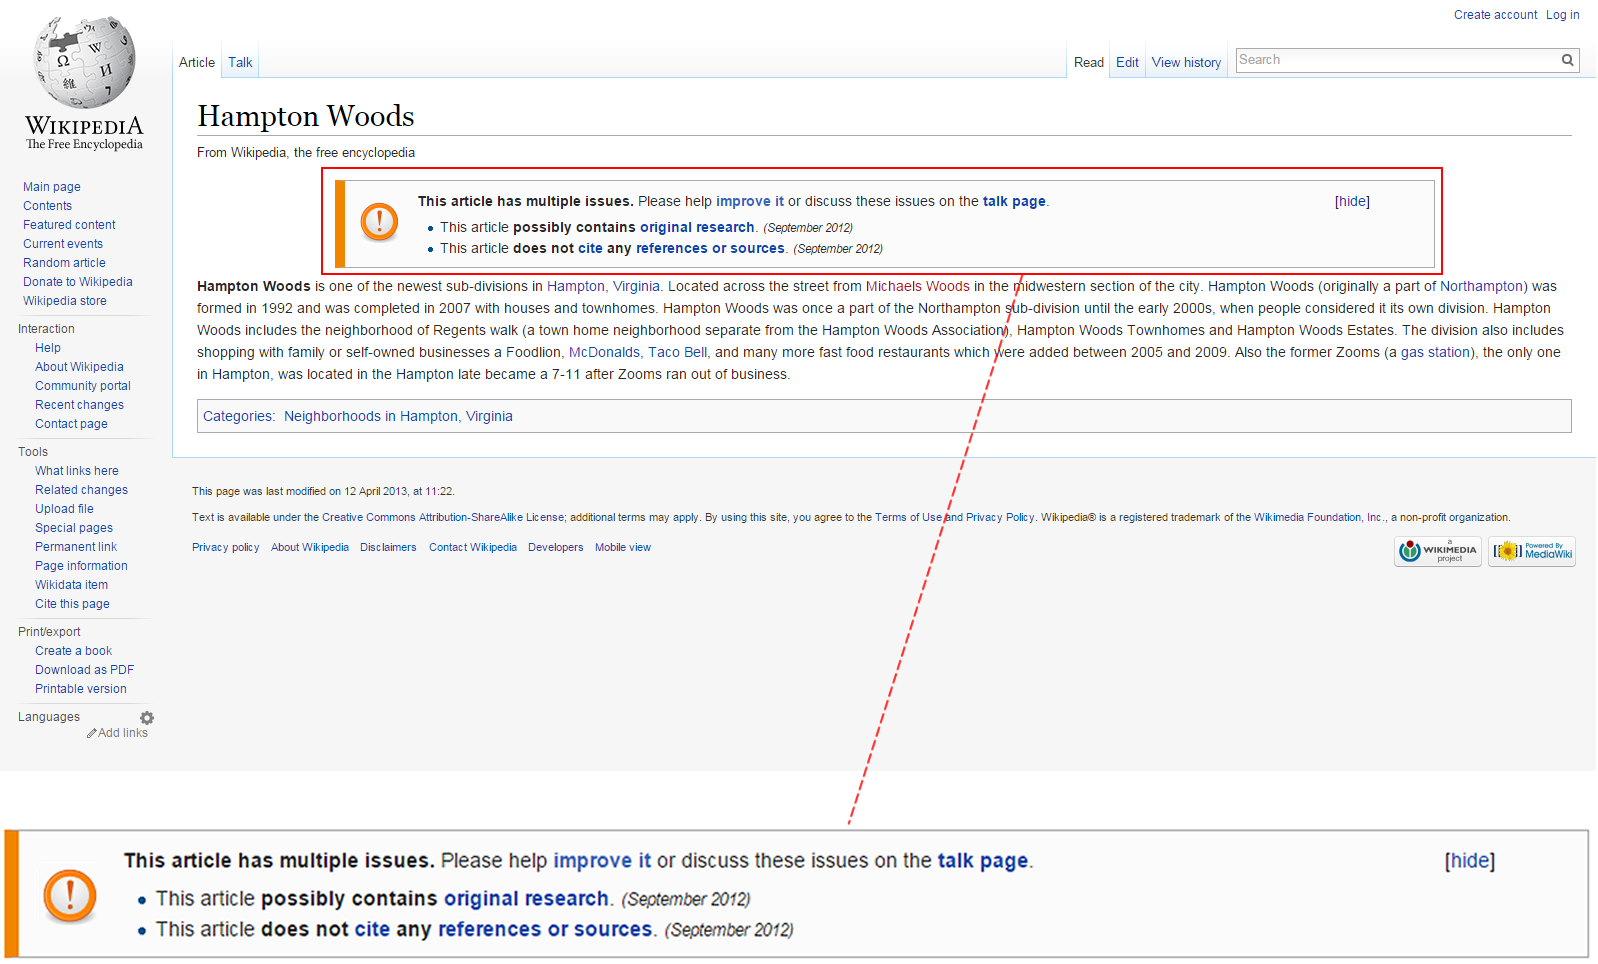
\includegraphics[width=1\textwidth]{imagenes/deteccion_falla3.png}
		\caption{Art\'iculo de Wikipedia ``Hampton Woods'' con la etiqueta \emph{investigaci\'on original} y \emph{falta de fuentes} }
		\label{fig:hamptonwood}
	\end{center}
\end{figure}

Si bien existen investigaciones que consideraron peque\~nas muestras de art\'iculos ~\cite{StTwSmGa:08} o analizaron un conjunto restringido de fallas de calidad ~\cite{AndSteLip:11, GaBeRoDa:09}, los pioneros en realizar un an\'alisis detallado fueron investigadores de la Universidad de Weimar, encabezado por Mike Anderka ~\cite{AndSte:10, AndSteBu:12, AndSteLip:12}. Este estudio revel\'o que un 27.52 \% de los art\'iculos de Wikipedia en Ingl\'es contiene al menos una falla de calidad y que un 70 \% corresponde a deficiencias de verificabilidad. Como se basaron en art\'iculos etiquetados manualmente, el porcentaje real, tiende a ser m\'as alto que el nombrado, por lo que existe la posibilidad de que muchos art\'iculos con deficiencias no hayan sido identificados todav\'ia ~\cite{PoFeErre:13}.

En el trabajo llevado a cabo por ~\cite{MaAn:13} se agrupan las 445 fallas nombradas anteriormente en 12 categor\'ias ya que varias fallas se relacionan al mismo tipo, por ejemplo, \emph{no referenciada} y \emph{necesita citas}, ambas se refieren a verificabilidad, una categor\'ia que hace alusi\'on a un documento que no presenta referencias. Como aporte principal de este trabajo, se propone una miner\'ia autom\'atica para extraer las etiquetas de limpieza de Wikipedia, las cuales nos dan el conjunto completo de las fallas de calidad identificadas por los usuarios de Wikipedia.  Esta organizaci\'on revela la estructura de las fallas de calidad de Wikipedia as\'i como tambi\'en indica la importancia de la misma.

En el cuadro ~\ref{tablatfp1} se muestra el agrupamiento de fallas determinado en dicha investigaci\'on,  su descripci\'on y cantidad de fallas de calidad relacionadas. A continuaci\'on se explican los 12 agrupamientos.

El primero, \emph{verificabilidad}, es uno de los principios m\'as importantes de una enciclopedia, y hace referencia a art\'iculos que no tienen referencias (\emph{sin referencias}, \emph{sin notas al pie de p\'agina}), son inadecuadas o inv\'alidas (\emph{fuentes primarias}, \emph{v\'inculo roto}) o simplemente que tienen declaraciones sin fuentes (\emph{necesita citas}, \emph{qui\'en} y \emph{por qui\'en}).

La falla \emph{estilo de escritura}, se refiere a caracter\'isticas estil\'isticas como gram\'atica, estilo, cohesi\'on, tono, etc, la mayor\'ia detallados en el manual de estilos de Wikipedia\footnote{Manual de estilos de Wikipedia. http://en.wikipedia.org/wiki/Wikipedia:Manual\_of\_Style.}.

El agrupamiento bajo el nombre \emph{miscel\'aneos}, comprende fallas que son muy espec\'ificas y que ocurren infrecuentemente.

Las fallas que surgen en un tema particular, se organizan bajo el tipo \emph{tema espec\'ifico}. Por ejemplo, la falla \emph{plot}, argumento, indica que el argumento de resumen podr\'ia ser muy extenso o excesivamente detallado, que s\'olo aplica a pel\'iculas o novelas.

La falla \emph{contenido no deseado} se refiere al contenido que no es apropiado por una enciclopedia (\emph{notabilidad}, \emph{publicidad}, \emph{investigaci\'on original}).

La falla \emph{neutralidad}, hace referencia a que el contenido es imparcial y sin opiniones, un elemento muy importante para una enciclopedia.

\emph{Wiki tech}, otro de los agrupamientos, hace alusi\'on a aspectos t\'ecnicos del art\'iculo, por ejemplo, que sea hu\'erfano, es decir, que no haya referencias a \'el o que no est\'e categorizado.

La falla \emph{limpieza general} agrupa las etiquetas de limpieza que listan varias fallas en una sola etiqueta (\emph{m\'ultiples cuestiones}) o simplemente requieren de una limpieza sin proveer mayor informaci\'on.

La falla \emph{ampliar}, indica que deben mejorarse ciertas secciones completando con mayor detalle o que cierta informaci\'on falta.

La falla \emph{estructura} nos determina que los art\'iculos deben estar organizados en secciones y con ciertas longitudes, etc.

Aquellos art\'iculos que est\'en determinados por el tiempo de vida o la actualidad deben estar organizados bajo la falla \emph{sensibilidad al tiempo}. Por \'ultimo, los art\'iculos que manejen temas similares deben ser combinados bajo la falla \emph{unir}.

De las 445 fallas de calidad, el trabajo nombrado se enfoca en las 10 fallas principales de la Wikipedia en Ingl\'es:
\begin{itemize}
\item 	No Referenciado: el art\'iculo no cita referencia o fuentes.
\item 	Hu\'erfano: se tiene menos de 3 enlaces entrantes en el art\'iculo.
\item 	Mejora de referencias: el art\'iculo necesita referencias adicionales para su verificaci\'on.
\item 	Secci\'on vac\'ia: el art\'iculo al menos tiene una secci\'on vac\'ia.
\item 	Notabilidad: el art\'iculo no cumple con la directriz general de notabilidad.
\item 	Sin nota de pie: no posee notas al pie de p\'agina.
\item 	Fuentes primarias: el art\'iculo se basa en referencias a las fuentes primarias.
\item 	Wikifi: el art\'iculo necesita ser wikificado (enlaces internos y  el dise\~no).
\item 	Anuncio: el art\'iculo est\'a escrito como un anuncio.
\item 	Investigaci\'on original: el art\'iculo contiene una investigaci\'on original.
\end{itemize}

En el estudio nombrado, se intent\'o determinar si un art\'iculo contiene o no una falla de calidad, dada una muestra de art\'iculos que contienen dicha falla. Se trat\'o el problema como uno de clase \'unica con el m\'etodo PU Learning (aprendizaje de ejemplos positivos y no etiquetados). Dicho m\'etodo utiliza un peque\~no conjunto de clases etiquetadas positivas, ninguna negativa (siendo \'este el mayor desaf\'io planteado) y un gran conjunto no etiquetado para ayudar a un modelo que se utiliza para predecir la presencia o no de la falla.

A modo de conclusi\'on, en los trabajos encabezados por Mike Anderka, se aborda la idea de fallas de calidad desde una perspectiva diferente a trav\'es del uso de etiquetas de limpieza, los cuales son indicadores de calidad de los art\'iculos, como se detall\'o en p\'arrafos anteriores. En una primera investigaci\'on ~\cite{AndSte:10} provee un desglose de las fallas de calidad de la Wikipedia en Ingl\'es, mientras que eval\'uan su eficacia para garantizar la calidad en ~\cite{AndSteBu:12} mediante el an\'alisis de la evoluci\'on de marcadores de fallas de calidad en el tiempo. Por \'ultimo, en ~\cite{AndSteLip:12}, los autores logran detectar autom\'aticamente fallas de calidad a trav\'es de la predicci\'on de etiquetas de limpieza en art\'iculos no vistos, lo cual coincide con la tarea planteada como objetivo en el desaf\'io PAN.

En la investigaci\'on ~\cite{OfIgMr:12} se propone un m\'etodo diferente, en \'el construyen un sistema llamado \emph{FlawFinder}, un sistema modular y flexible para predecir autom\'aticamente fallas de calidad en art\'iculos de Wikipedia a trav\'es de cinco componentes los cuales podr\'ian trabajar de manera independiente tambi\'en; un lector de corpus, un preprocesador, una unidad de extracci\'on de caracter\'isticas, un m\'odulo para entrenamiento y un escritor de reportes.

Como caracter\'istica destacable de este trabajo de investigaci\'on, \'este sistema, en vez de leer los datos de entrenamiento proporcionados por la competencia PAN, en la cual obtuvo la mejor precisi\'on de todos los sistemas expuestos y el segundo puesto en cuanto a recall y F1, directamente el lector de corpus accede a los art\'iculos desde a la base de Wikipedia creada por ellos mismos, la cual posee un amplio rango de meta datos tales como estructura de v\'inculos e informaci\'on acerca del historial de revisi\'on de los art\'iculos ~\cite{OfIgMr:12}.

\section{Visualizaci\'on} 
\chapter{Detalles de implementaci\'on}

\section{Introducci\'on}

En el siguiente cap\'itulo describiremos los detalles del trabajo realizado, desde la estructuraci\'on de las fuentes de datos utilizados, hasta la implementaci\'on de los algoritmos de b\'usqueda. Dado que el objetivo principal de este trabajo es determinar (a trav\'es de la aplicaci\'on a un caso de uso real) qu\'e estrategia de selecci\'on de pivotes es la mejor, nos restringimos a implementar el m\'etodo b\'asico de b\'usqueda que puede utilizarse desde cualquier tipo de sistema: sitio web, aplicaci\'on de tel\'efono celular, etc.\\

Para el desarrollo del software seleccionamos el framework Grails (versi\'on 1.3.7), que contiene el lenguaje Groovy para la codificaci\'on y Java para la ejecuci\'on.\\

Todas las estructuras de datos fueron manejadas en memoria principal, tanto para la creaci\'on de \'indices como para las b\'usquedas.


\section{Procesamiento inicial de los datos de entrada} \label{proc-inic}

Cuando hablamos de datos de entrada, nos referimos a los productos ofrecidos en el sitio Mercado Libre (a los que tambi\'en llamaremos items). Estos productos est\'an clasificados dentro de un \'arbol de categor\'ias, donde cada categor\'ia re\'une productos relacionados. Remitiendonos a los n\'umeros, obtuvimos alrededor de 2 millones de productos, distribuidos en 12.000 categor\'ias (hojas).\\

La informaci\'on relevante a \'este trabajo obtenida de los productos fue la siguiente: categor\'ia, identificador del producto, t\'itulo, descripci\'on principal y descripci\'on secundaria.\\

Para optimizar el desarrollo de creaci\'on de \'indices, los datos de entrada tuvieron que ser pre procesados de manera de crear los archivos necesarios para el correcto funcionamiento de dicho proceso. De este pre procesamiento obtuvimos:

\begin{enumerate}[1.]
\item  Archivo de productos: texto plano conteniendo toda la informaci\'on pertinente de los productos, separada por comas.
\item  Archivo de categor\'ias: texto plano conteniendo el nombre de la categor\'ia.
\item  Archivo de productos divididos por categor\'ia: archivo de datos serializados, conteniendo un mapa cuyas claves son las categor\'ias y cuyo valor es la lista de productos correspondiente, conteniendo informaci\'on m\'inima para la selecci\'on de pivotes: identificador del producto y codificaci\'on del t\'itulo (la codificaci\'on consiste en eliminar caracteres especiales, reemplazar vocales acentuadas por no acentuadas, suprimir espacios superfluos y pasar a may\'usculas el t\'itulo completo).
\end{enumerate}

\section{Estructuras de datos}

Para el almacenamiento de las categor\'ias se implement\'o un rebalse abierto lineal con un factor de carga de \textit{0,4}. Cada elemento del rebalse se compone de una estructura que contiene el nombre de la categor\'ia y una lista de firmas. Cada firma representa la distancia de edici\'on de cada t\'itulo del \'item a cada t\'itulo del elemento pivote, e incluye el identificador de \'item en cuesti\'on.\\

Para el resto de las estructuras auxiliares utilizamos un mapa, estructura de datos que provee el lenguaje utilizado. En dicha estructura se almacenan pares de $(clave,valor)$ y posteriormente puede realizarse la evocaci\'on del valor utilizando la clave.\\

Para el almacenamiento de los datos completos del producto se utiliz\'o un mapa cuya clave es el identificador y el valor asociado es una estructura que contiene la totalidad de los datos del producto.\\

Como \'ultima estructura de datos auxiliar, se eligi\'o un mapa cuya clave es la categor\'ia y el valor asociado es la lista de pivotes correspondiente, conteniendo solo el identificador del producto y la codificaci\'on del t\'itulo.\\



\begin{figure}[H]
\centering
\subfigure[\scriptsize Rebalse de categor\'ias]{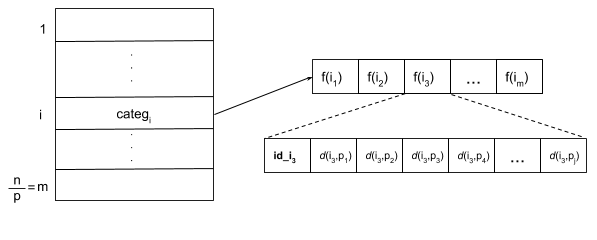
\includegraphics[width=90mm]{imagenes/estructuras/categs-hash.png}}
\subfigure[\scriptsize Mapa de productos]{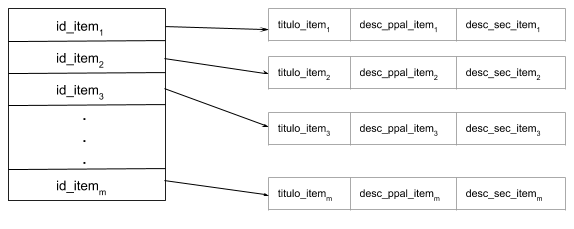
\includegraphics[width=90mm]{imagenes/estructuras/map-items.png}}
\subfigure[\scriptsize Mapa de pivotes por categor\'ias]{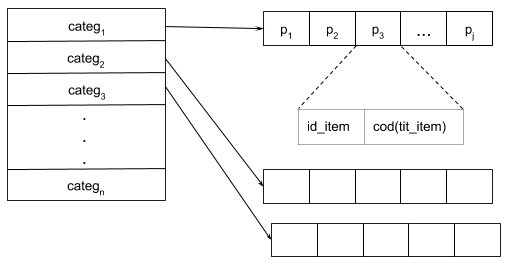
\includegraphics[width=90mm]{imagenes/estructuras/categs-pivots.png}}
    \caption{\small Estructuras de datos utilizadas}
    \label{fig:estructuras}
\end{figure}

\section{Software desarrollado}

El desarrollo realizado consta de dos partes complementarias: la funcionalidad de creaci\'on de \'indices y la funcionalidad de b\'usqueda propiamente dicha, que utiliza los \'indices creados por la primera funcionalidad.\\

\subsection{Creaci\'on de \'indices para las b\'usquedas}

La funcionalidad de creaci\'on de \'indices se desarroll\'o en forma gen\'erica, preparada para recibir los siguientes par\'ametros: \textit{tipo de pivotes} (aleatorio o incremental), \textit{cantidad de pivotes} y \textit{conjunto de pivotes} (pudiendo elegirse entre el mismo conjunto para todas las categor\'ias o diferentes conjuntos para cada categor\'ia).\\

B\'asicamente el algoritmo de creaci\'on realiza la carga de los archivos descritos en la secci\'on  \ref{proc-inic} en las estructuras de datos correspondientes, y procede a generar las firmas de los items; utilizando, en primera instancia, la estrategia de selecci\'on de pivotes en conjunci\'on con el resto de los par\'ametros (cantidad y conjunto de pivotes).\\

Luego de completar la estructura con las firmas de los items, almacena cada estructura en un archivo de datos serializados; para que puedan ser utilizados en futuras b\'usquedas.\\

\begin{algorithm}[caption={Creaci\'on de \'indice}, label={alg1}]
crearIndice(File fCategs, File fPivs, String estSel, int cantPivs)
begin
 /* Se inicializan las estructuras */
 Hash categsHash = inicializarHashCategorias(fCategs)
 Map pivotesPorCateg
 /* Se obtiene el conjunto de pivotes en base a la estrategia */
 if(estSel == "aleatorio")
 begin
  pivotesPorCateg = obtConjPivsAleatorio(fPivs, cantPivs)
 end

 if(estSel == "incremental")
 begin
  pivotesPorCateg = obtConjPivsIncremental(fPivs, cantPivs)
 end

 Map items
 /*Se calculan las firmas para todos los items*/
 forall item in archivoItems
 begin
  Pivotes pivs = pivotesPorCateg.get(item.categ)
  Dist[] d = calcularDistancias(item.cod_titulo, pivotes)
  categsHash.get(item.categ).add(d)
  items.put(item.id, item)
 end
 /* Se almacenan las estructuras que componen el indice en archivos 
  * para su utilizacion futura */
 generarArchivoSerializado(categsHash)
 generarArchivoSerializado(pivotesPorCateg)
 generarArchivoSerializado(items)
end
\end{algorithm}

A continuaci\'on se presenta el pseudo-c\'odigo de los algoritmos de selecci\'on de pivotes. Para facilitar la lectura de los mismos solo se incluy\'o la variante de distinto conjunto de pivotes para cada categor\'ia.

\begin{algorithm}[caption={Selecci\'on de pivotes aleatoria}, label={alg2}]
obtConjPivsAleatorio(File fPivs, int cantPivs)
begin
 Map conjuntoFinal
 Map pivotesPorCateg = obtenerPivotesPorCateg(fPivs)
 for(categ, pivotes in pivotesPorCateg)
 begin
  /* Se eliminan elementos aleatoriamente hasta 
   * alcanzar la cantidad de pivotes deseada */
  while(pivotes.size > cantPivs)
  begin
   eliminarElementoAleatorio(pivotes)
  end
  conjuntoFinal.put(categ, pivotes)
 end
 return conjuntoFinal
end
\end{algorithm}

\begin{algorithm}[caption={Selecci\'on de pivotes incremental}, label={alg3}]
obtConjPivsIncremental(File fPivs, int cantPivs)
begin
 Map conjuntoFinal
 Map pivotesPorCateg = obtenerPivotesPorCateg(fPivs)
 for(categ, pivotes in pivotesPorCateg)
 begin
  conjuntoPivotes
  int candidato, selec
  float dim, max
  for(i = 1 to cantPivs)
  begin
   /* Se elige un candidato inicial */ 
   selec = random(n)
   while(selec ya haya sido elegido antes)
    selec = random(n)
   conjuntoPivotes->puntos[i] = pivotes->puntos[selec]
   /* 10 es la cantidad de pares de elementos para el calculo
    * de la media D */
   max = mediaD(conjuntoPivotes, 10)
   candidato = selec
   for j = 2 to 10
    begin
    /* Se busca nuevo cantidato */
    selec = random(n)
    while(selec ya haya sido escogido antes)
     selec=random(n)
    conjuntoPivotes->puntos[i] = pivotes->puntos[selec]
    /* 10 es la cantidad de pares de elementos para el calculo 
     * de la media D */
    dim = mediaD(conjuntoPivotes, 10)
    if(dim > max)
    begin
     max = dim
     candidato = selec
    end
   end
   conjuntoPivotes->puntos[i] = pivotes->puntos[candidato]
  end
  conjuntoFinal.put(categ, pivotes)
 end
 return conjuntoFinal
end
\end{algorithm}

Como se puede inferir entonces, el algoritmo de creaci\'on de indices particiona el universo de datos $\mathcal{U}$ (los productos) a trav\'es de las categor\'ias hojas, resultando en multiples $U_i$ listas que potencialmente contienen elementos relevantes para una consulta.\\

\subsection{Busqueda por similitud}

Se implementaron dos funcionalidades de b\'usqueda: b\'usqueda por rango, que recibe por par\'ametro el radio de b\'usqueda, la categor\'ia del producto y el t\'itulo de un producto existente; y b\'usqueda de los k-vecinos, que recibe por par\'ametro la cantidad de elementos a retornar (k), la categor\'ia del producto y el t\'itulo de un producto existente.\\

La b\'usqueda por rango calcula la distancia del t\'itulo del producto dado por par\'ametro a cada uno de los pivotes, y luego compara esa firma contra las firmas de los productos de la categor\'ia seleccionada. Este paso retorna los productos candidatos a formar parte de la respuesta final, los cuales son utilizados para calcular la distancia real de edici\'on contra el producto buscado, descartando aquellos que est\'en fuera del rango especificado.\\

\begin{algorithm}[caption={B\'usqueda por rango}, label={alg4}]
busquedaPorRango(String q, String categ, int radio)
begin
 Pivotes pivotes = pivotesPorCateg.get(categ)
 /* Se calcula la firma para la query */
 Dist[] d = calcularDistancia(q, pivotes)
 List candidatos = []
 /* Se obtienen todas las firmas para la categoria */
 List[Dist[]] firmas = categsHash.get(categ)
 /* Se compara la firma de la query con las firmas de la categoria, 
  * si el valor es mayor que el radio, se descarta el item */
 for(j = 0 to firmas.size)
 begin
  int[] dists = firmas[j].dists
  boolean agregar = true
  for (i = 0 to dists.size)
  begin
   int value = valorAbsoluto(sig.dists[i] - dists[i])
   if (value > radio)
   begin
    i = dists.size
    agregar = false
   end
  end
  if(agregar)
   candidatos.add(firmas[j])
 end
 List itemsEncontrados = []
 for(i = 0 to candidatos.size)
 begin
  Item item = items.get(candidatos[i].id)
  int dist = distanciaEdicion(q, item.cod_titulo)
  if((radio - dist) > 0)
   itemsEncontrados.add(item)
 end
 return itemsEncontrados
end
\end{algorithm}

La b\'usqueda de los k-vecinos utiliza una variaci\'on de la b\'usqueda por rango, comenzando con un valor inicial $v$ para el radio e incrementando ese valor hasta llegar a la cantidad deseada de resultados.\\
\begin{algorithm}[caption={B\'usqueda de los k-vecinos}, label={alg5}]
busquedaKVecinos(String q, String categ, int radio, int k)
begin
 int radio = 0
 int i = 1
 List resultadoFinal
 List itemsTemp = []
 while(itemsTemp.size < k)
 begin
  radio = potencia(5,i)
  itemsTemp = busquedaPorRango(q, categ, radio)
  /* Si se obtuvieron mas elementos que el k deseado, se procede 
   * a realizar una biseccion del radio */
  if(itemsTemp.size > k)
  begin
   int li = potencia(5,i - 1)
   int ls = radio
   /* Se realiza una biseccion del radio */
   while(li <= ls)
   begin
    radio = ((ls + li)/2)
    itemsTemp = busquedaPorRango(q, categ, radio)
    /* Se alcanzo el numero deseado de elementos, se finaliza la biseccion */
    if(itemsTemp.size == k)
    begin
     li = ls + 1
     resultadoFinal = itemsTemp
    end
    /* Se continua la biseccion para uno u otro lado, dependiendo 
     * de si se supero o no la cantidad de elementos */
    else
    begin
     if(itemsTemp.size < k)
     begin
      li = radio + 1
      radio = radio + 1
     end
     else
      ls = radio - 1
    end
   end
   if(itemsTemp.size != k)
   begin
    /* Si el ultimo resultado de la biseccion obtuvo menos elementos,
     * se debe hacer la busqueda con el valor final del radio */
    if(itemsTemp.size < k)
     itemsTemp = busquedaPorRango(q, categ, radio)
    /* Se ordenan los elementos por su distancia y se seleccionan los k primeros */
    ordenarPorMenorDistancia(itemsTemp)
    resultadoFinal = itemsTemp.subList(0,k)
   end
  end
  else
   resultadoFinal = itemsTemp
  i = i + 1 
 end
 return resultadoFinal
end
\end{algorithm}

Como funcionalidad auxiliar, se implement\'o un proceso de carga que puede ser utilizado al iniciar el programa, para cargar los archivos de \'indices previamente generados.


\section{Re-particionado del universo}

Luego de planificar, diseñar e implementar todas las estructuras de datos, realizamos pruebas manuales para asegurarnos del correcto funcionamiento del software completo.\\

Ante estas pruebas, detectamos que el particionado no era sem\'anticamente correcto, ya que al elegir la categor\'ia hoja del \'arbol, estabamos restringiendo demasiado el universo de b\'usqueda.\\

Representando la situaci\'on con un ejemplo, supongamos que deseamos recomendar productos similares al producto \textit{“Samsung Galaxy A30 32 GB Blanco 3 GB RAM”}, la categor\'ia hoja de dicho producto es \textit{“A30”}, dentro del \'arbol: \textit{“Celulares y Tel\'efonos > Celulares y Smartphones > Samsung > A30”}, si solo tenemos en cuenta los productos que pertenecen a la categor\'ia \textit{“A30”}, es probable que no encontremos, por ejemplo, celulares blancos de 32 GB de la marca Motorola.
Por \'este motivo, definimos volver a particionar el universo de productos, \'esta vez utilizando la categor\'ia inicial del \'arbol (Celulares y Tel\'efonos en el ejemplo anterior).\\

Con \'esta nueva estrategia, obtuvimos 30 particiones distintas de nuestro universo, para las cuales realizamos los experimentos descritos en el pr\'oximo cap\'itulo.

\chapter{Evaluaci\'on experimental}

En este cap\'itulo presentamos los resultados de ejecutar el algoritmo de b\'usqueda por rango usando dos t\'ecnicas de selecci\'on de pivotes: random y incremental.\\

Comenzaremos describiendo el seteo experimental, los experimentos realizados y luego daremos el an\'alisis de los resultados obtenidos.\\

En una primera etapa nos enfocamos en determinar el rango adecuado para las b\'usquedas y la forma en que \'ibamos a seleccionar los conjuntos de pivotes para cada una de las t\'ecnicas de selecci\'on.\\

\section{Seteo Experimental}

Para los experimentos usamos la base de datos de "\textit{items}" (productos publicados) de Mercadolibre.\\
	
Agrupamos los productos en categor\'ias que re\'unen productos de similares caracter\'isticas, teniendo como resultado 30 categor\'ias distintas, que de  ahora en adelante las llamaremos bases de datos.\\

Por cada base de datos y por cada t\'ecnica de selecci\'on, random e incremental, creamos \'indices y files de pivotes. Los n\'umeros de pivotes elegidos fueron: 16, 32, 64, 128, 256, 512, 1024, 2048 y 4096. Los pivotes seleccionados fueron obtenidos por categor\'ias. Para tomar esta decisi\'on hicimos experimentos que m\'as adelante mostraremos.\\

Luego, agrupamos las bases de datos en grupos segmentados seg\'un el procentaje que representan el n\'umero de pivotes sobre el tama\~no de la base de datos, a este valor lo llamaremos ratio de pivotes. Esto es as\'i porque tenemos bases de datos que son muy chicas (ejemplo: 1034 items) y el ratio de pivotes era muy alto para esas categor\'ias. De esta segmentaci\'on obtuvimos 4 grupos.\\

\subsection{Selecci\'on del rango de b\'usqueda}

La mayor\'ia de los trabajos de investigaci\'on existentes sobre b\'usqueda por similitud en textos, utilizan como universo de datos diccionarios de palabras como por ejemplo ingl\'es o español. Esto genera una base com\'un que puede utilizarse a la hora de generar variaciones sobre algoritmos de b\'usqueda en nuevos trabajos, es decir, se comparte la base de datos y los par\'ametros de los experimentos, lo cual permite poder comparar f\'acilmente los resultados de los mismos.\\
 
Es com\'un encontrar trabajos de b\'usqueda por rango donde la variaci\'on del radio es siempre entre 1 y 5 y la elecci\'on de ese valor no requiere m\'as que una simple decisi\'on azarosa por parte del autor.\\

En nuestro trabajo, el universo de datos es bastante m\'as singular, ya que se trata de t\'itulos de productos reales, cuya redacci\'on est\'a a cargo del usuario que publica el producto para su venta y donde la \'unica limitante es el tama\~no de ese t\'itulo (60 caracteres).\\

Esta particularidad tiene como consecuencia un universo de datos variado y heterog\'eneo, donde cada elemento de dicho universo es una combinaci\'on de palabras, abreviaciones, n\'umeros y caracteres especiales. Ante \'esta combinaci\'on de caracter\'isticas, el primer obst\'aculo que debimos sortear para comenzar con la evaluaci\'on experimental fue, precisamente, la selecci\'on del radio de b\'usqueda.\\

Como una primera aproximaci\'on, seleccionamos cuatro t\'itulos de productos (cuadro: \ref{tabla:muestra-rank}) de la categor\'ia con mayor cantidad de elementos (cuadro: \ref{tabla:muestra-tamano}) y luego procedimos a realizar una b\'usqueda de los k-vecinos con:\\

\begin{itemize}
\item $k= 0.001 \times  cantidad\_de\_elementos\_de\_la\_categoria\ (0.1\%)$
\item $k= 0.01 \times cantidad\_de\_elementos\_de\_la\_categoria\ (1\%)$
\item $k= 0.1 \times cantidad\_de\_elementos\_de\_la\_categoria\ (10\%)$
\end{itemize}

Las b\'usquedas se realizaron utilizando la estrategia de selecci\'on de pivotes incremental, y la cantidad de pivotes elegida fue de 128.\\

\begin{table}[H]
\begin{center}
\begin{tabular}{|c|c|c|c|}
\hline \multirow{2}{5cm}{\small Tama\~no de base de datos}
& \multicolumn{3}{p{4cm}|}
{\centering \small N\'umero de k-vecinos}\tabularnewline \cline{2-4}
& \multicolumn{1}{p{1.2cm}|}
{\centering \small 0.001\%}
& \multicolumn{1}{p{1.2cm}|}
{\centering \small 0.01\%}
& \multicolumn{1}{p{1.2cm}|}
{\centering \small 0.1\%}
\tabularnewline \hline
\hline
\small 31.632 & 32 & 316 & 3163 \\ \hline
\end{tabular}
\caption{\small N\'umero de k-vecinos utilizados.}
\label{tabla:muestra-tamano}
\end{center}
\end{table}

\begin{table}[H]
\begin{center}
\begin{tabular}{|l|c|c|c|}
\hline \multirow{2}{5cm}{\small T\'itulos de b\'usqueda}
& \multicolumn{3}{p{4cm}|}
{\centering \small Radio promedio}\tabularnewline \cline{2-4}
& \multicolumn{1}{p{1.2cm}|}
{\centering \small 0.001\%}
& \multicolumn{1}{p{1.2cm}|}
{\centering \small 0.01\%}
& \multicolumn{1}{p{1.2cm}|}
{\centering \small 0.1\%}
\tabularnewline \hline
\hline
\small Libro Te Amo Pero Soy Feliz Sin Ti. Jaime Jaramillo & 32 & 35 & 37 \\ \hline
\small El Secreto Rhonda Byrne Lvbp13 & 21 & 24 & 26 \\ \hline
\small Libro De Italiano Forza 2 & 14 & 17 & 23 \\ \hline
\small Libro La Magia Rhonda Byrne El Secreto Lvbp13 & 28 & 32 & 35 \\ \hline
\end{tabular}
\caption{\small Muestra para determinar el radio de b\'usqueda.}
\label{tabla:muestra-rank}
\end{center}
\end{table}

\begin{table}[H]
\begin{center}
\begin{tabular}{|l|c|}
\hline 
\small T\'itulos de b\'usqueda
&
\small Radio Promedio\\
\hline \hline
\small Libro Te Amo Pero Soy Feliz Sin Ti. Jaime Jaramillo & 32  \\ \hline
\small El Secreto Rhonda Byrne Lvbp13 & 21  \\ \hline
\small Libro De Italiano Forza 2 & 14  \\ \hline
\small Libro La Magia Rhonda Byrne El Secreto Lvbp13 & 28  \\ \hline  \hline
\hspace{4cm}  \textbf{\small PROMEDIO GENERAL} & \textbf{27} \\ \hline
\end{tabular}
\caption{\small Tabla de radio promedio.}
\label{tabla:promedios-rank}
\end{center}
\end{table}

Como podemos visualizar en los resultados de la tabla \ref{tabla:promedios-rank}, el promedio del radio de b\'usqueda arroja un valor de 27, valor que utilizamos para realizar algunas pocas b\'usquedas sobre el resto de las categor\'ias. Al analizar los resultados obtenidos llegamos a la conclusi\'on de que deb\'iamos disminu\'ir el valor del $r$, ya que en la mayor\'ia de los casos la b\'usqueda retornaba una cantidad de elementos cercana a la totalidad de la base de datos y en otros casos los elementos retornados no eran similares al t\'itulo de b\'usqueda. Ante \'estos hallazgos, tomamos una segunda aproximaci\'on: primero obtuvimos el promedio de la longitud de los t\'itulos para cada categor\'ia, luego promediamos esos valores para obtener un \'unico resultado y lo dividimos por 2.  De esa forma llegamos al rango elegido para todos los experimentos: $r=23$.\\


\subsection{Selecci\'on de los conjuntos de pivotes}

En este trabajo, adem\'as de las t\'ecnicas de selecci\'on de pivotes, random e incremental, consideramos dos pol\'iticas para la elecci\'on de los grupos de pivotes:\\

\textit{\textbf{Mismo grupo de pivotes para todas las categor\'ias o bases de datos}}: Esta estrategia, selecciona el grupo de pivotes considerando todas las bases de datos. Luego, el mismo grupo de pivotes, es utilizado en cada uno de los experimentos sobre las distintas bases de datos.\\

\textit{\textbf{Diferentes grupos de pivotes por categor\'ia o base de datos}}: Sobre cada una de las bases de datos se seleccionan los conjuntos de pivotes.\\

Para determinar cu\'al estrategia era la m\'as adecuada, se seleccionaron conjuntos de pivotes, random e incremental, seg\'un las pol\'iticas arriba mencionadas para los grupos de 16 y 64 pivotes.\\

Por cada base de datos se eligi\'o al azar el 10\% de los t\'itulos como elementos de b\'usqueda. Para las b\'usquedas con 16 pivotes, se usaron 6 bases de datos (tamaño total: 61.184) y se ejecutaron 12.232  b\'usquedas en total. Para las b\'usquedas con 64 pivotes, se usaron 18 bases de datos (tamaño total: 440.631) y se ejecutaron un total de 88.114 b\'usquedas.\\

En la figura \ref{fig:same-vs-diff-16Pivotes}, se muestra el ratio de comparaciones para las b\'usquedas con 16 pivotes. Para la t\'ecnica de selecci\'on incremental (a) se puede observar que se comporto mejor la pol\'itica \textit{Mismo grupo de pivotes para todas las categor\'ias o bases de datos} y para la t\'ecnica de selecci\'on random (b) fue mejor la pol\'itica \textit{Diferentes grupos de pivotes por categor\'ia o base de datos}.\\

En la figura \ref{fig:same-vs-diff-64Pivotes}, se visualiza el ratio de comparaciones para las b\'usquedas con 64 pivotes. Para ambas t\'ecnica de selecci\'on, incremental (a) y random (b), se puede observar que se comporto mejor la pol\'itica \textit{Diferentes grupos de pivotes por categor\'ia o base de datos}. Esto es, el ratio de comparaciones realizadas directamente con los objetos de la base de datos es menor al usar diferentes pivotes por categor\'ia o base de datos.\\

\begin{figure}[tb]
\centering
\subfigure[\scriptsize T\'ecnica de selecci\'on incremental]{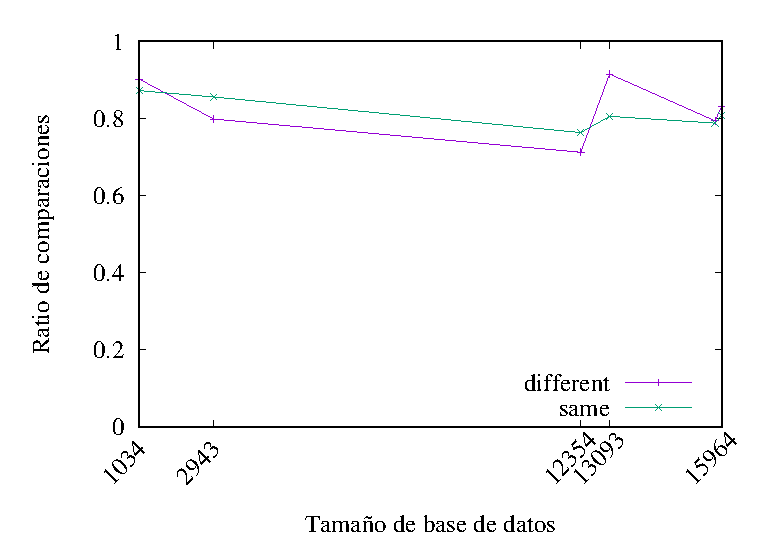
\includegraphics[width=71.5mm]{imagenes/same_vs_different/16p_incremental.eps}}
\subfigure[\scriptsize T\'ecnica de selecci\'on random]{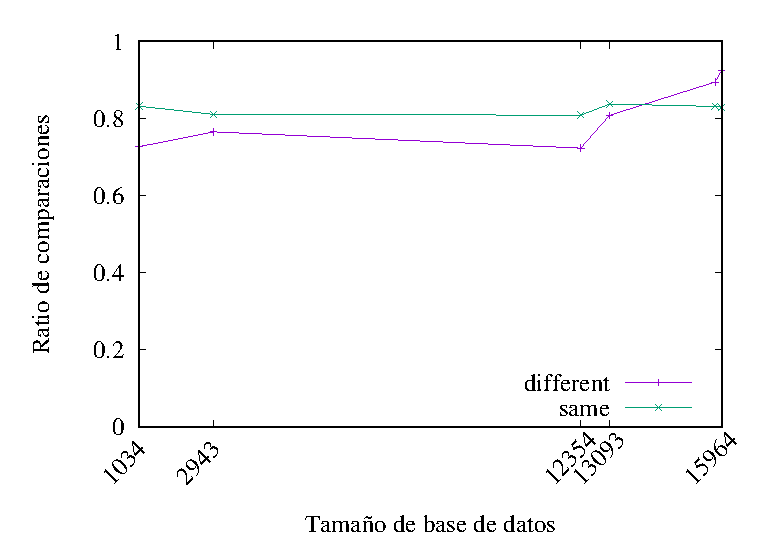
\includegraphics[width=71.5mm]{imagenes/same_vs_different/16p_random.eps}}
		\caption{\small Estrategia de selecci\'on para 16 pivotes: mismos pivotes vs diferentes}
		\label{fig:same-vs-diff-16Pivotes}
\end{figure}

\begin{figure}[tb]
\centering
\subfigure[\scriptsize T\'ecnica de selecci\'on incremental]{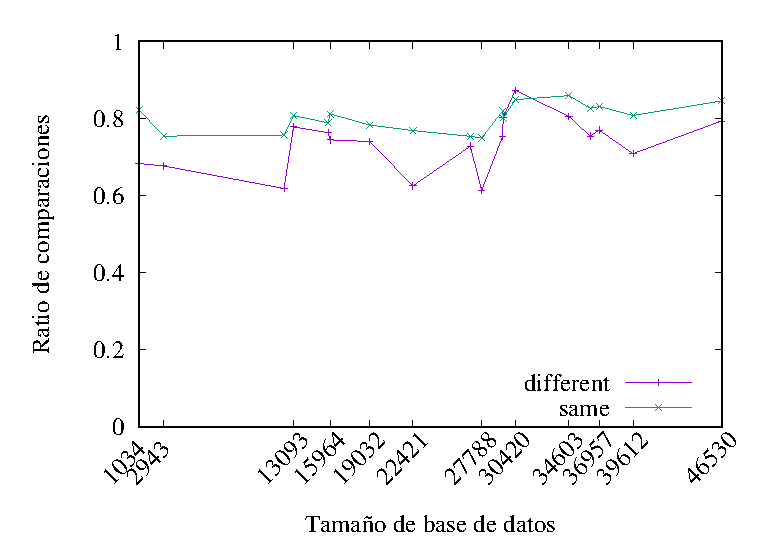
\includegraphics[width=71.5mm]{imagenes/same_vs_different/64p_incremental.eps}}
\subfigure[\scriptsize T\'ecnica de selecci\'on random]{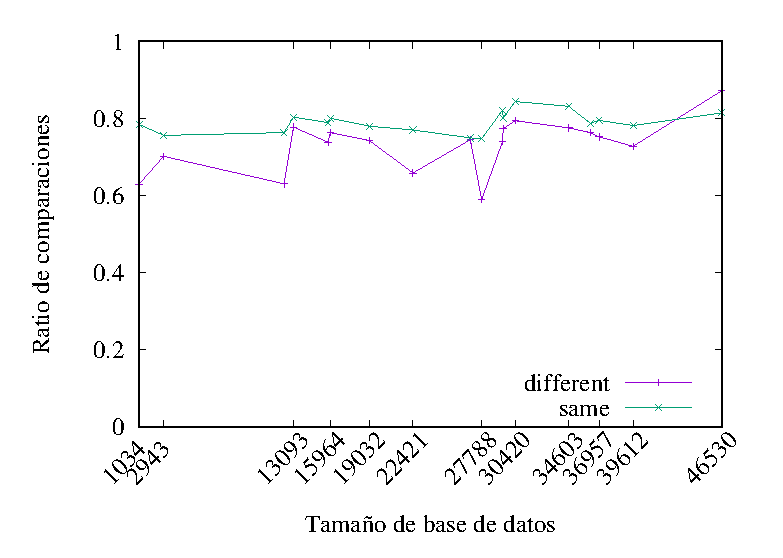
\includegraphics[width=71.5mm]{imagenes/same_vs_different/64p_random.eps}}
		\caption{\small Estrategia de selecci\'on para 64 pivotes: mismos pivotes vs diferentes}
		\label{fig:same-vs-diff-64Pivotes}
\end{figure}

\section{Ejecuci\'on experimental}

En una segunda etapa,  nos concentramos en c\'omo agrupar los datos teniendo en cuenta la variaci\'on del tama\~no de las bases de datos para luego poder analizar la informaci\'on segmentada y poder sacar mejores conclusiones.\\

\subsection{Creaci\'on de grupos}

Dada la variabilidad de tamaños de las bases de datos, para poder analizar luego los resultados correctamente, definimos cuatro grupos segmentados por el tamaño de base de datos y por cantidad de pivotes. Esto es, calculamos el ratio de pivotes sobre el tamaño de las base de datos (DB), quedando la siguiente distribuci\'on:\\

\begin{table}[htbp]
\begin{center}
\begin{tabular}{|p{1.1cm}|p{1.8cm}|p{3.2cm}|p{2.2cm}|p{2.5cm}|}
\hline
Grupo & 
Cantidad de DB & 
Rango del tama\~no de DB & 
N\'umero de Pivotes &  
Cantidad de Experimentos\\
\hline \hline
1 & 
6 & 
[1.034 - 15.964] & 
16, 32, 64, 128, 256 & 
60  \\ \hline
2 &
12 &
[19.032 - 46.530] &
64, 128, 256, 512, 1024 &
120  \\ \hline
3 &
8 &
[57.198 - 13.6323] &
256, 512, 1024, 2048 &
64  \\ \hline
4 &
4 &
[16.7995- 21.3578] &
512, 1024, 2048, 4096 &
32  \\ \hline
\end{tabular}
\caption{Tabla de grupos.}
\label{tabla:grupos}
\end{center}
\end{table}

En total se ejecutaron 276 experimentos. Esto es, 138 experimentos usando t\'ecnica de selecci\'on de pivotes random y 138 experimentos usando t\'ecnica de selecci\'on de pivotes incremental.\\

Se seleccion\'o al azar el 10\% de los elementos de cada una de las bases de datos para realizar las b\'usquedas. La cantidad total de b\'usquedas por rango realizadas fue: 339.899. Este valor incluye las b\'usquedas usadas para descartar la pol\'itica de selecci\'on \textit{Mismo grupo de pivotes para todas las categor\'ias o bases de datos} mencionada anteriormente.\\

\section{An\'alisis de resultados}

Vamos a presentar los resultados segmentados en cuatro grupos y analizaremos tres enfoques diferentes.\\

Llamaremos ratio de comparaciones al porcentaje de comparaciones respecto del tamaño de la base de datos, esto es porcentaje de filtrado.\\

\subsection{Efecto de las t\'ecnicas de selecci\'on de pivotes}

En esta secci\'on vamos a comparar las t\'ecnicas de selecci\'on de pivotes random e incremental, usando como m\'etrica el n\'umero de evaluaciones de distancia para cada unos de los grupos de pivotes elegidos. Se realizaron las comparaciones para todas las bases de datos con las que trabajamos (30) pero a continuaci\'on s\'olo analizaremos la base de datos de mayor tama\~no de cada uno de los grupos que mencionamos anteriormente, el resto se adjuntan en el Anexo \ref{anexo.A}.\\

Para el grupo 1, figura \ref{fig:ETS-1}(a), observamos que para una base de datos de aproximadamente 16 mil elementos,  usando la t\'ecnica de selecci\'on incremental se realizan menos evaluaciones de distancia que la t\'ecnica de selecci\'on random para todos los grupos de pivotes, excepto para 128 pivotes. Tambi\'en se puede observar que la diferencia entre ambas t\'ecnicas es amplia.\\

Para el grupo 2, figura \ref{fig:ETS-1}(b), para una base de datos de aproximadamente 45 mil elementos, la t\'ecnica de selecci\'on incremental es mejor solo en dos grupos de pivotes, 64 y 256. Para los grupos de pivotes de 128, 512 y 1024, la t\'ecnica de selecci\'on random realiza menos evaluaciones de distancia que incremental. Tambi\'en se puede observar que a partir del grupo de pivotes 256, la diferencia de evaluaciones de distancia no es tan grande entre ambas t\'ecnicas.\\

Para el grupo 3, figura \ref{fig:ETS-2}(a), con una base de datos de aproximadamente 136 mil elementos, la t\'ecnica de selecci\'on incremental en general realiza menos cantidad de evaluaciones de distancia, salvo para 2048 pivotes. Para este ultimo grupo de pivotes, la t\'ecnica de selecci\'on random esta por debajo de incremental pero solo por muy poca diferencia.\\

Para el grupo 4, figura \ref{fig:ETS-2}(b), con una base de datos de aproximadamente 213 mil elementos, en general, la t\'ecnica de selecci\'on random, por muy poca diferencia (excepto para 4096, donde la diferencia es mas marcada), realiza menos cantidad de evaluaciones de distancia que la t\'ecnica de selecci\'on incremental.\\


\begin{figure}[tb]
\centering
\subfigure[\scriptsize Grupo 1]{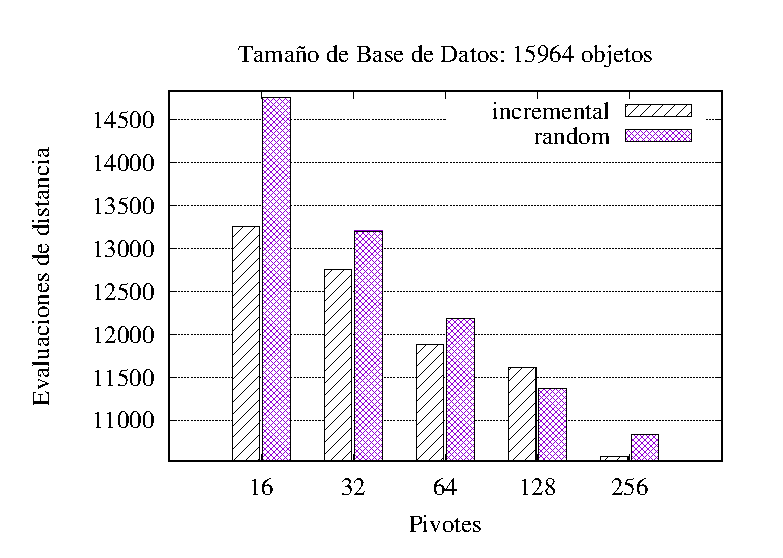
\includegraphics[width=71.5mm]{imagenes/random_vs_incremental/g1_15964.eps}}
\subfigure[\scriptsize Grupo 2]{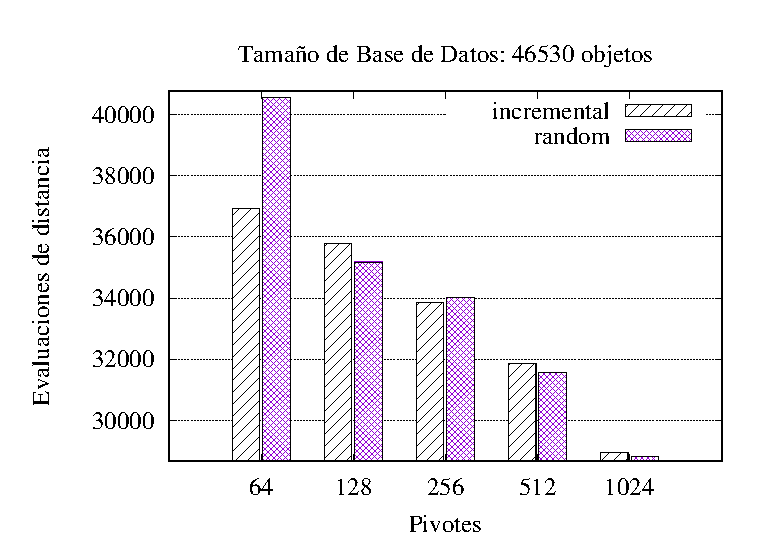
\includegraphics[width=71.5mm]{imagenes/random_vs_incremental/g2_46530.eps}}
\caption{\small Efecto de las t\'ecnicas de selecci\'on de pivotes random vs incremental respecto de evaluaciones de distancia.}
\label{fig:ETS-1}
\end{figure}
\begin{figure}[tb]
\centering
\subfigure[\scriptsize Grupo 3]{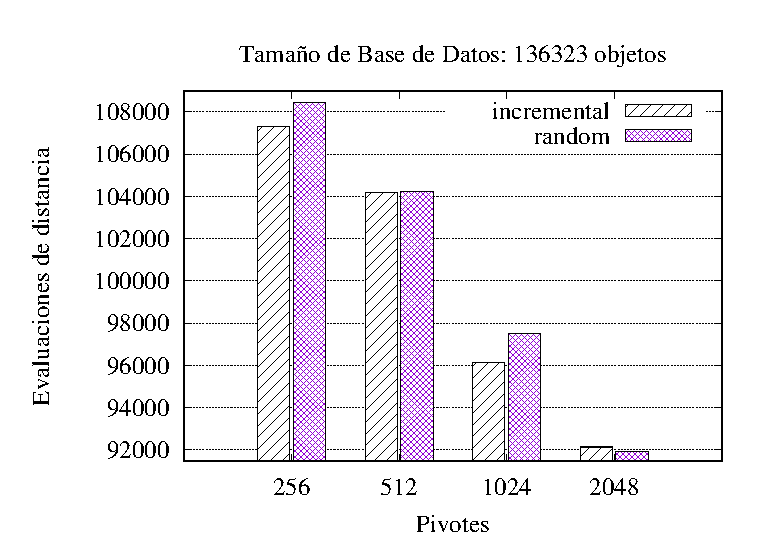
\includegraphics[width=71.5mm]{imagenes/random_vs_incremental/g3_136323.eps}}
\subfigure[\scriptsize Grupo 4]{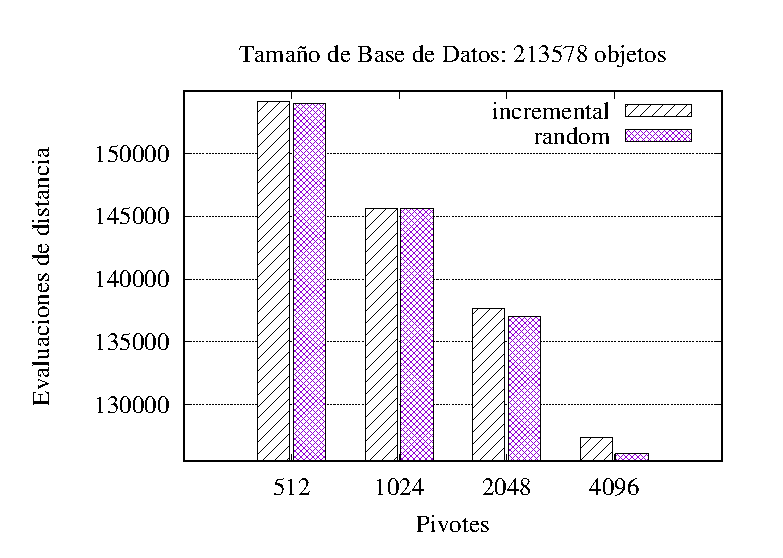
\includegraphics[width=71.5mm]{imagenes/random_vs_incremental/g4_213578.eps}}
\caption{\small Efecto de las t\'ecnicas de selecci\'on de pivotes random vs incremental respecto de evaluaciones de distancia.}
\label{fig:ETS-2}

\end{figure}

Como conclusi\'on general, se puede observar que la t\'ecnica de selecci\'on random realiza menos cantidad de evaluaciones de distancia, aunque por muy poca diferencia.\\
 
Dado que el comportamiento para ambas t\'ecnicas de selecci\'on no era el que esperabamos, es decir, incremental no era mucho mejor que random en cuanto a ratio de comparaciones, hicimos un an\'alisis emp\'irico sobre diferentes categor\'ias para entender tal comportamiento. Este an\'alisis lo veremos mas adelante en detalle (\ref{capitulo.H}).

\subsection{Efecto de la cantidad de pivotes}

A continuaci\'on vamos a analizar el efecto de la cantidad de pivotes sobre el ratio de comparaciones para cada base de datos. Cada l\'ineas representa una base de datos y estas bases de datos est\'an representadas por su tamaño como se muestra en las gr\'aficas.\\

En la figura \ref{fig:EP-g1}, observamos que tanto para selecci\'on de pivotes random (a) como para selecci\'on de pivotes incremental (b), para $16, 32, 64, 128$ y $256$ pivotes, a media que aumenta el n\'umero de pivotes el ratio de comparaciones disminuye. Tambi\'en vemos que las 3 bases de datos mas grandes, tienen un comportamiento similar, es decir el ratio de comparaciones oscila entre $0,7$ y $0,93$ aproximadamente y para las 3 bases de datos mas chicas, oscila entre $0,4$ y $0,8$ aproximadamente.\\

En la figura \ref{fig:EP-g2}, observamos que para los pivotes $64, 128, 256, 512$ y $1024$ ambas t\'ecnicas de selecci\'on de pivotes se comportan semejantes, a mayor n\'umero de pivotes menor ratio de comparaciones. El ratio de comparaciones est\'a entre $0,6$ y $0,8$ para todas las bases de datos excepto la $27788$ que se encuentra entre $0,4$ y $0,6$.\\

En la figura \ref{fig:EP-g3}, observamos el mismo comportamiento que para los grupos 1 y 2 mencionados anteriormente. En ambas t\'ecnicas de selecci\'on de pivotes, para la mayor\'ia de las bases de datos el ratio de comparaciones est\'a entre $0,6$ y $0,8$. Para pivotes de este grupo, $256, 512, 1024$ y $2048$, tambi\'en, a mayor n\'umero de pivotes menor ratio de comparaciones.\\

En la figura \ref{fig:EP-g4}, observamos que a media que aumenta el n\'umero de pivotes el ratio de comparaciones disminuye, similar al resto de los grupos. Tambi\'en vemos que 3 de las 4 bases de datos que estamos analizando, para los pivotes 512, 1024 y 2048; el ratio de comparaciones esta entre $0,6$ y $0,75$ aproximadamente y para 4096 pivotes, entre $0,5$ $0,6$.\\

A modo de resumen, analizando el efecto de la cantidad de pivotes en general para los cuatro grupos, vemos que cuando aumenta el n\'umero de pivotes se decrementa el ratio de comparaciones pero las t\'ecnicas de selecci\'on random e incremental, no muestran diferencias entre ellas.

\begin{figure}[tb]
\centering
\subfigure[\scriptsize T\'ecnica de selecci\'on de pivotes random]{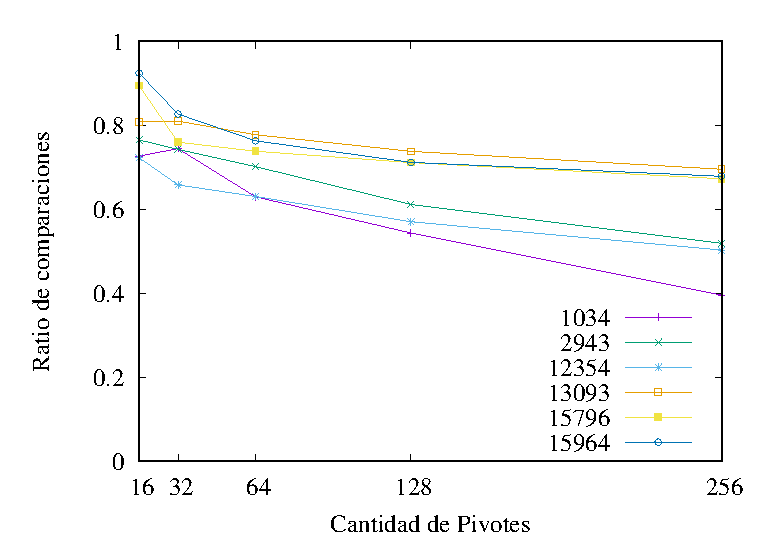
\includegraphics[width=71.5mm]{imagenes/efecto_pivotes/g1_random_ep.eps}}
\subfigure[\scriptsize T\'ecnica de selecci\'on de pivotes incremental]{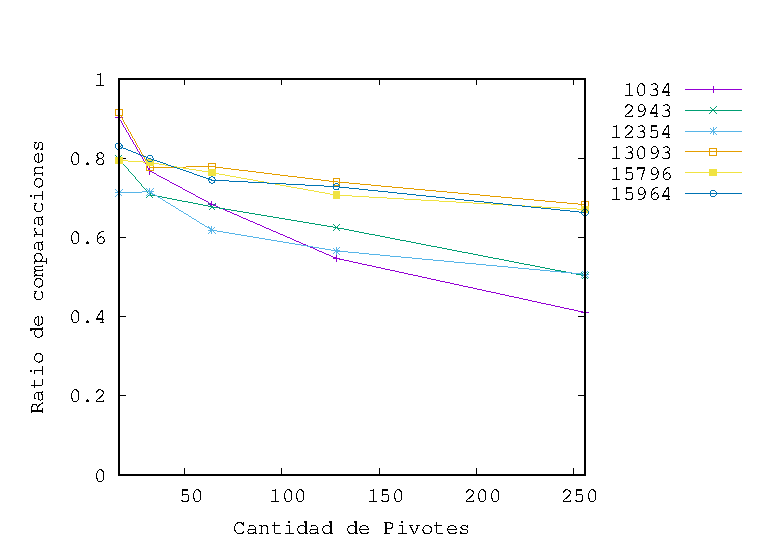
\includegraphics[width=71.5mm]{imagenes/efecto_pivotes/g1_incremental_ep.eps}}
		\caption{\small Grupo 1 - Efecto de la cantidad de pivotes sobre el ratio de comparaciones.}
		\label{fig:EP-g1}
\end{figure}

\begin{figure}[H]
\centering
\subfigure[\scriptsize T\'ecnica de selecci\'on de pivotes random]{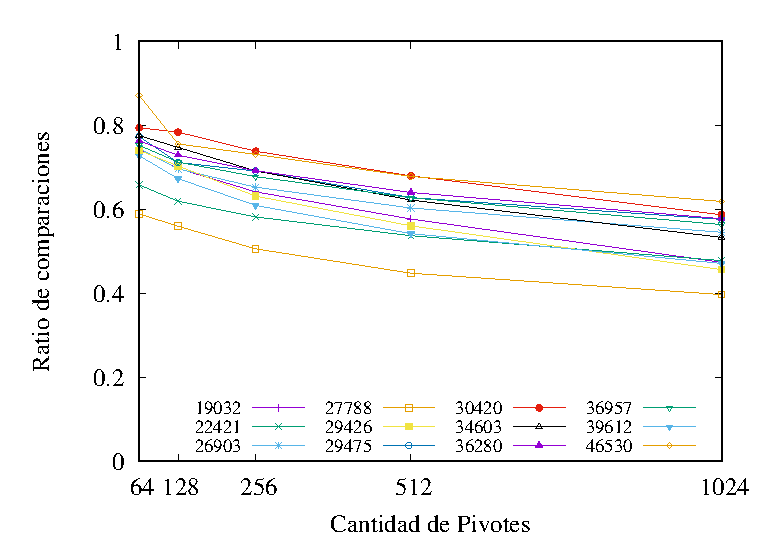
\includegraphics[width=71.5mm]{imagenes/efecto_pivotes/g2_random_ep.eps}}
\subfigure[\scriptsize T\'ecnica de selecci\'on de pivotes incremental]{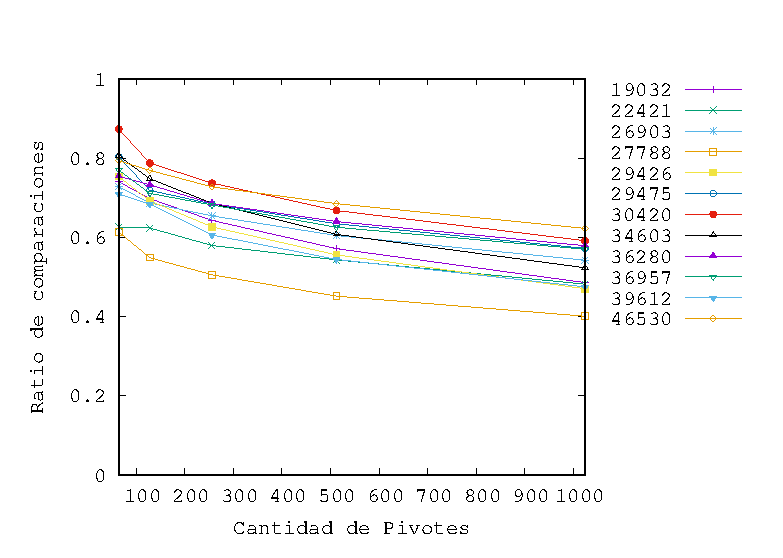
\includegraphics[width=71.5mm]{imagenes/efecto_pivotes/g2_incremental_ep.eps}}
		\caption{\small Grupo 2 - Efecto de la cantidad de pivotes sobre el ratio de comparaciones.}
		\label{fig:EP-g2}
\end{figure}

\begin{figure}[tb]
\centering
\subfigure[\scriptsize T\'ecnica de selecci\'on de pivotes random]{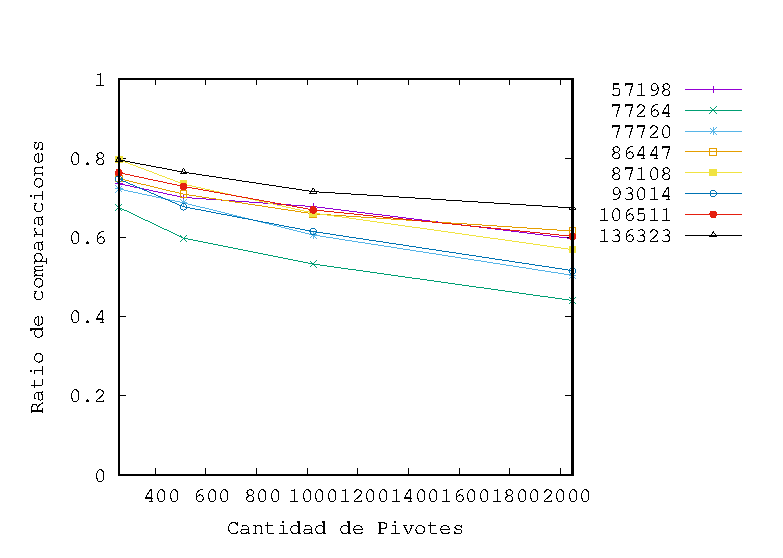
\includegraphics[width=71.5mm]{imagenes/efecto_pivotes/g3_random_ep.eps}}
\subfigure[\scriptsize T\'ecnica de selecci\'on de pivotes incremental]{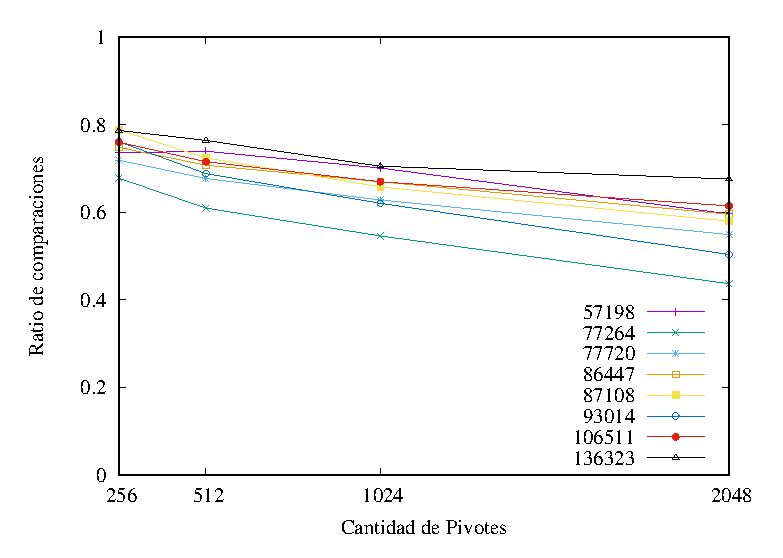
\includegraphics[width=71.5mm]{imagenes/efecto_pivotes/g3_incremental_ep.eps}}
		\caption{\small Grupo 3 - Efecto de la cantidad de pivotes sobre el ratio de comparaciones.}
		\label{fig:EP-g3}
\end{figure}

\begin{figure}[tb]
\centering	
\subfigure[\scriptsize T\'ecnica de selecci\'on de pivotes random]{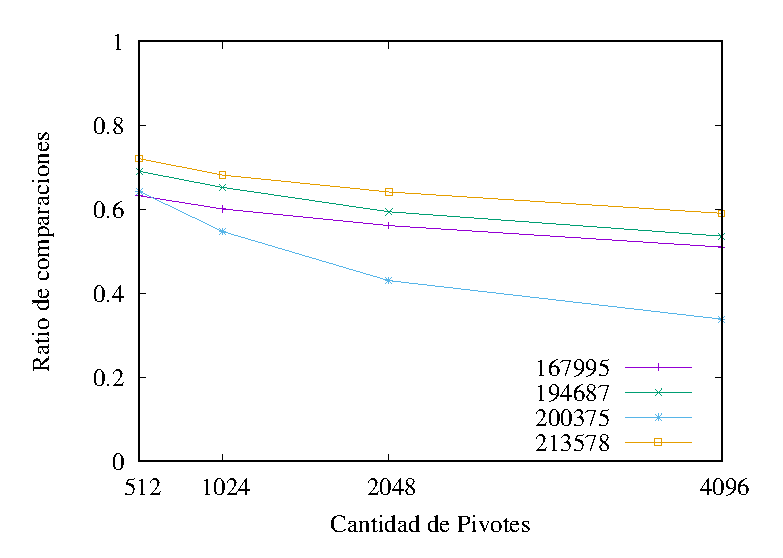
\includegraphics[width=71.5mm]{imagenes/efecto_pivotes/g4_random_ep.eps}}
\subfigure[\scriptsize T\'ecnica de selecci\'on de pivotes incremental]{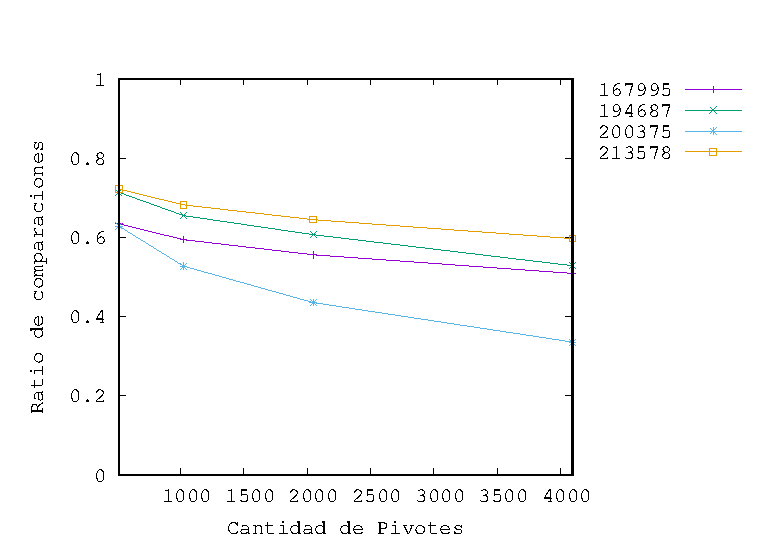
\includegraphics[width=71.5mm]{imagenes/efecto_pivotes/g4_incremental_ep.eps}}
		\caption{\small Grupo 4 - Efecto de la cantidad de pivotes sobre el ratio de comparaciones.}
		\label{fig:EP-g4}
\end{figure}

\subsection{Efecto tamaño de la base de datos}

\begin{figure}[tb]
\centering
\subfigure[\scriptsize T\'ecnica de selecci\'on de pivotes random]{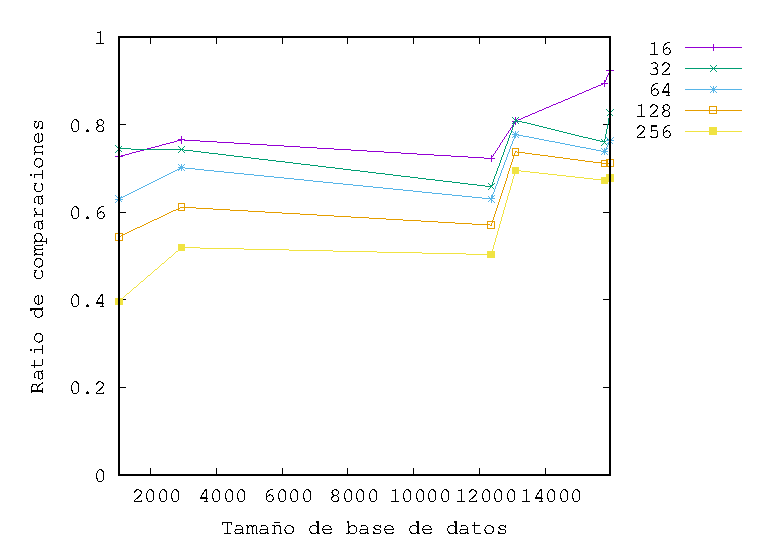
\includegraphics[width=71.5mm]{imagenes/efecto_db/g1_random_edb.eps}}
\subfigure[\scriptsize T\'ecnica de selecci\'on de pivotes incremental]{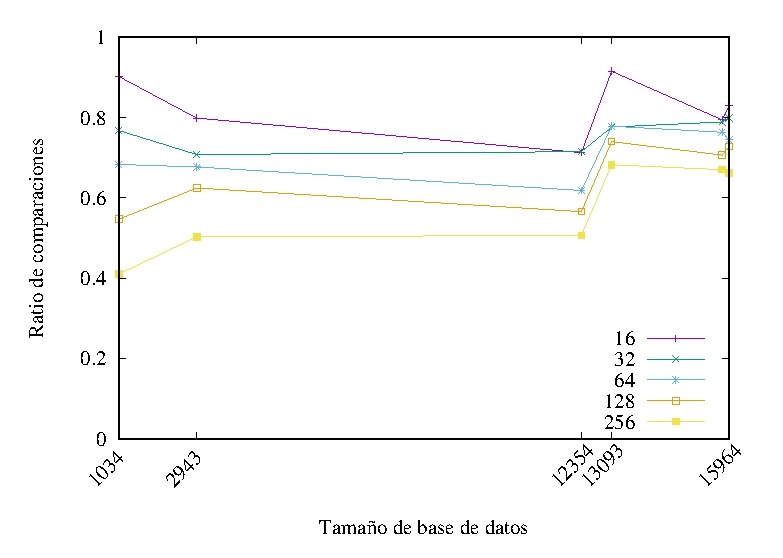
\includegraphics[width=71.5mm]{imagenes/efecto_db/g1_incremental_edb.eps}}
		\caption{\small Grupo 1 - Efecto del tamaño de la base de datos sobre el ratio de comparaciones por pivotes.}
		\label{fig:EDB-g1}
\subfigure[\scriptsize T\'ecnica de selecci\'on de pivotes random]{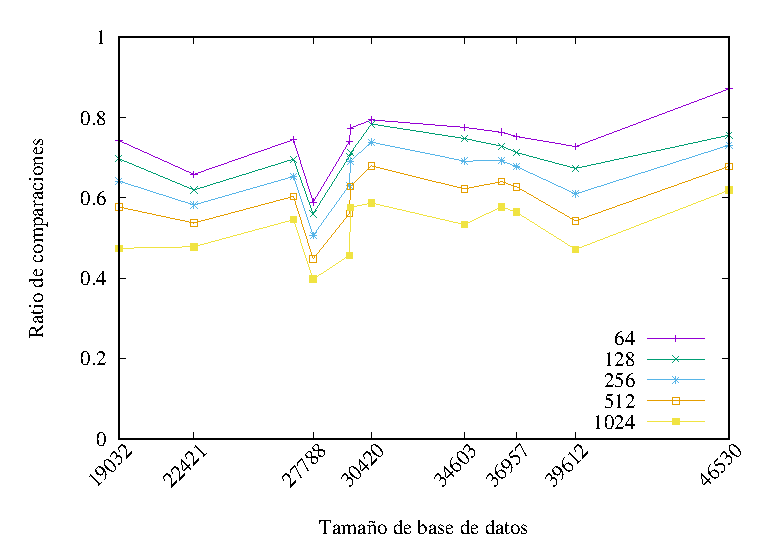
\includegraphics[width=71.5mm]{imagenes/efecto_db/g2_random_edb.eps}}
\subfigure[\scriptsize T\'ecnica de selecci\'on de pivotes incremental]{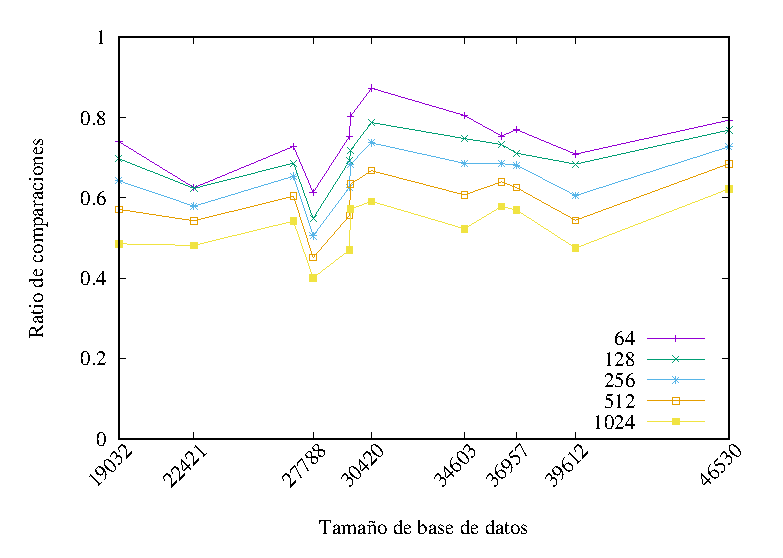
\includegraphics[width=71.5mm]{imagenes/efecto_db/g2_incremental_edb.eps}}
		\caption{\small Grupo 2 - Efecto del tamaño de la base de datos sobre el ratio de comparaciones por pivotes.}
		\label{fig:EDB-g2}
\end{figure}

\begin{figure}[tb]
\centering
\subfigure[\scriptsize T\'ecnica de selecci\'on de pivotes random]{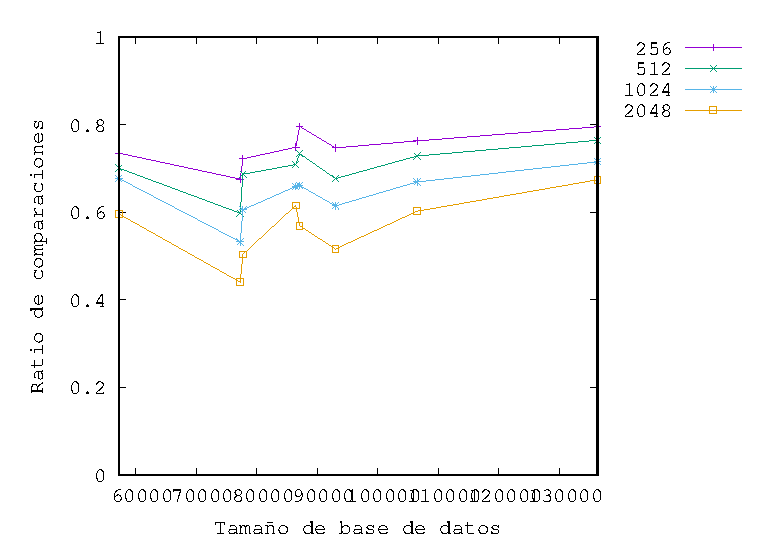
\includegraphics[width=71.5mm]{imagenes/efecto_db/g3_random_edb.eps}}
\subfigure[\scriptsize T\'ecnica de selecci\'on de pivotes incremental]{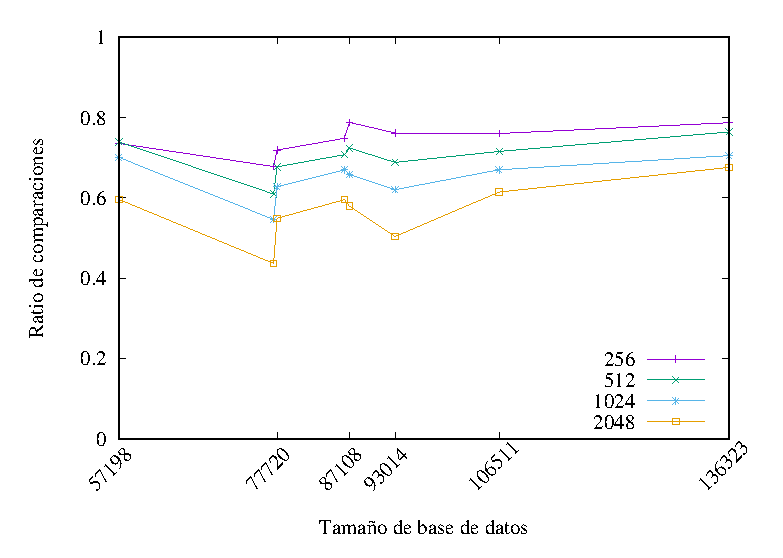
\includegraphics[width=71.5mm]{imagenes/efecto_db/g3_incremental_edb.eps}}
		\caption{\small Grupo 3 - Efecto del tamaño de la base de datos sobre el ratio de comparaciones por pivotes.}
		\label{fig:EDB-g3}
\end{figure}

\begin{figure}[tb]
\centering
\subfigure[\scriptsize T\'ecnica de selecci\'on de pivotes random]{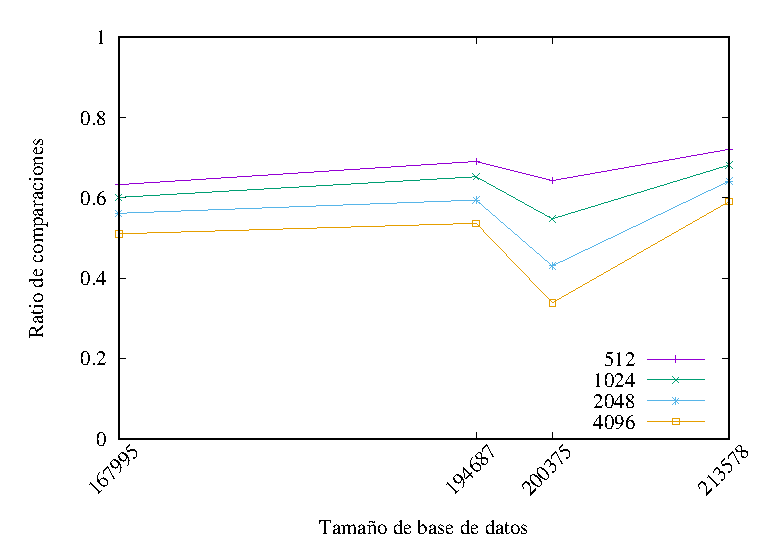
\includegraphics[width=71.5mm]{imagenes/efecto_db/g4_random_edb.eps}}
\subfigure[\scriptsize T\'ecnica de selecci\'on de pivotes incremental]{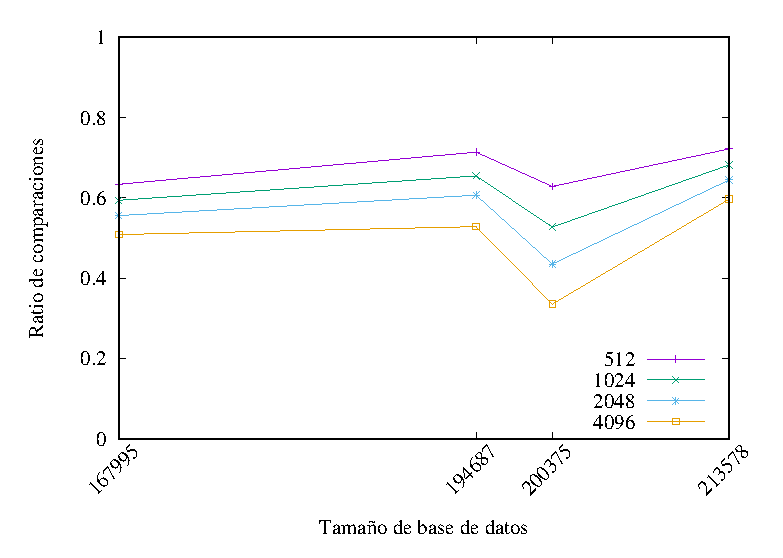
\includegraphics[width=71.5mm]{imagenes/efecto_db/g4_incremental_edb.eps}}
		\caption{\small Grupo 4 - Efecto del tamaño de la base de datos sobre el ratio de comparaciones por pivotes.}
		\label{fig:EDB-g4}
\end{figure}
 
A continuaci\'on vamos a analizar cual es el efecto del tama\~no de las bases de datos sobre el ratio de comparaciones por pivotes. Las l\'ineas de las graficas son el n\'umero de pivotes con los que se ejecutaron las b\'usquedas.\\

En la figura \ref{fig:EDB-g1} tenemos el grupo 1; donde el rango del tama\~no de las bases de datos es $[1.034-15.964]$ y los pivotes usados son $16, 32, 64, 128$ y $256$. Para la t\'ecnica de selecci\'on de pivotes random (a), en la base de datos mas chica, el ratio de comparaciones esta entre $0,4$ y $0,8$ y para las base de datos m\'as grandes, entre $0,7$ y $0,9$. Por otro lado, si miramos la gr\'afica para $256$ pivotes podemos observar que para las base de datos mas chica el ratio de comparaciones es $0,4$ y a medida que crece en tama\~no de la base de datos el ratio de comparaciones tambien aumenta ($0,7$ en las bases de datos mas grandes).\
Para la t\'ecnica de selecci\'on de pivotes incremental (b), el comportamiento es similar, a menor cantidad de pivotes, mayor ratio de comparaciones.\\

En la figura \ref{fig:EDB-g2}, donde el tama\~no de las bases de datos van desde $19032$ a $46530$ elementos y los pivotes usados son $64, 128, 256, 512$ y $1024$, el ratio de comparaciones no tiene mucha variabilidad desde la base de datos mas chica a las mas grande.\
Por ejemplo: para t\'ecnica de selecci\'on de pivotes random, 512 pivotes y una bade de datos de 19 mil elementos el ratio de comparaciones es $0,58$ aproximadamente y para una base de datos de 46 mil elementos, el ratio es $0,67$. Estos valores son similares para el caso de t\'ecnica de selecci\'on de pivotes incremental.\
A nivel general, para t\'ecnica de selecci\'on de pivotes random, podemos ver que para la base de datos mas chica, el ratio de comparaciones varia entre 0,49 y 0,79; y para las base de datos mas grande, entre 0,6 y 0,84. Para t\'ecnica de selecci\'on de pivotes incremental los rangos de ratios de comparaciones estan entre $[0,5 - 0,77]$ y $[0,61 - 0,79]$. \\

Para las figuras \ref{fig:EDB-g3} y \ref{fig:EDB-g4}, donde se muestran los grupos 3 y 4 respectivamente, el comportamiento es similar al de los grupos antes mencionados.	\
A medida que el tama\~no de las base de datos aumenta, el ratio de comparaciones tambi\'en crece, aunque la variabilidad de este \'ultimo es muy baja. Esto es similiar en ambas  t\'ecnica de selecci\'on de pivotes.

 \section{Histogramas de frecuencia}\label{capitulo.H}
 
Cuando comenzamos a analizar algunos resultado, vimos que el comportamiento no era el que esperabamos. Al comparar las  t\'ecnica de selecci\'on incremental y random, identificamos que no hab\'ia un mejora significativa en cuanto a la cantidad o ratio de comparaciones. Ade\'mas los algotirtmos de b\'usqueda no performaban bien en cuanto al tiempo de ejecución.\\

Dado que cada base de datos, es un universo completamente distinto y que en todos los casos vimos el mismo comportamiento calculamos los histogramas de frecuencia para todas las bases de datos. Todos los histogramas se adjuntan en el Anexo \ref{anexo.B}.\\\\

En la figuras \ref{fig:HF1} y \ref{fig:HF2} se puede observar como lo elementos se encuentran concentrados, lo cual se asemejan a un histogragma de alta dimensionalidad como vimos en la figura \ref{dim1} (p\'agina \pageref{dim1}).\\

Esto significa como mencionamos anteriormente que a medida que los elementos se encuentran mas concentrados al rededor de su media, disminuye la cantidad de elementos que pueden ser descartados. Esto es, aumenta la cantidad de comparaciones con elementos de base de datos.\\

Si analizamos nuevamente las figuras \ref{fig:EP-g4} y \ref{fig:EDB-g4} que muestran el efecto de la cantidad de pivotes y el efecto del tama\~no de la base de datos respectivamente, para ambos casos independientemente de la t\'ecnica de selecci\'on, vemos que el ratio de comparaciones para 4096 pivotes o para la base de datos mas grande ronda el 0,6 equivalente al 60	\%.\\

Como s\'intensis, vemos en general que no hay una mejora al comparar las t\'ecnicas de selecci\'on y que el porcentaje de comparaciones con los elementos de la base de datos es elevado.\\

\begin{figure}[tb]
\centering
\subfigure{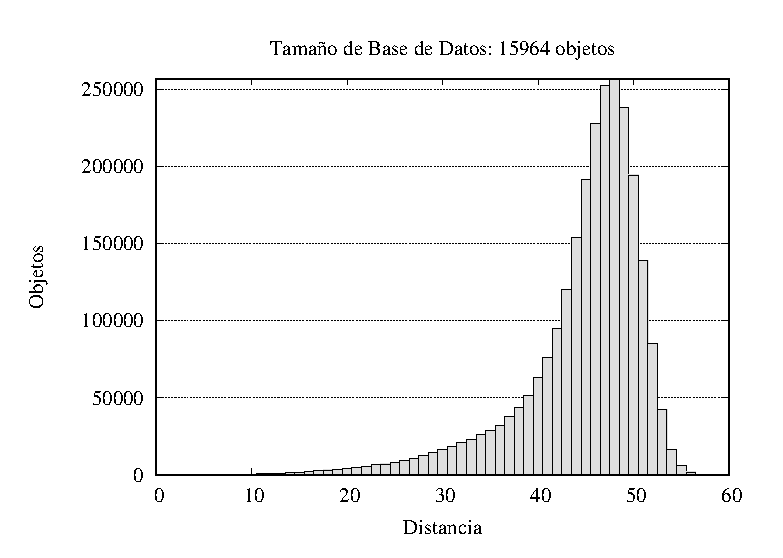
\includegraphics[width=71.5mm]{imagenes/histogramas/31928_items.eps}}
\subfigure{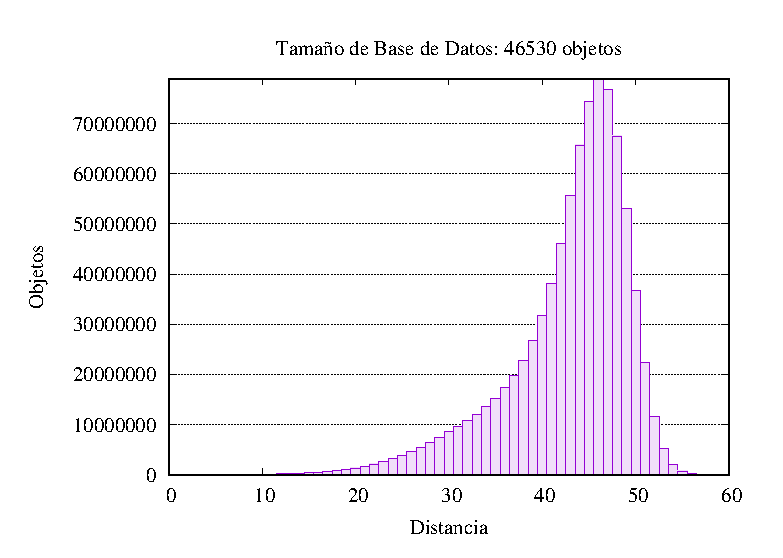
\includegraphics[width=71.5mm]{imagenes/histogramas/93060_items.eps}}
		\caption{\small Histogramas de frecuencia de la base de datos m\'as grandes del grupo 1 (izquierda) y del grupo 2 (derecha).}
		\label{fig:HF1}
		
\subfigure{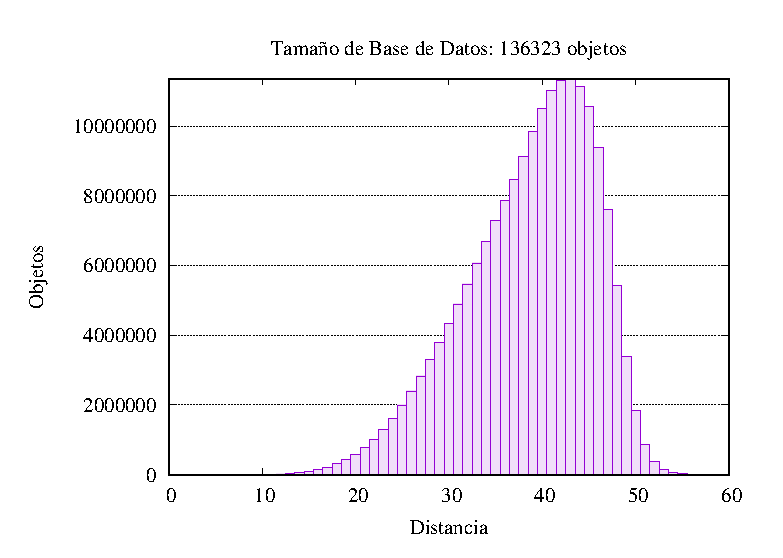
\includegraphics[width=71.5mm]{imagenes/histogramas/272646_items.eps}}
\subfigure{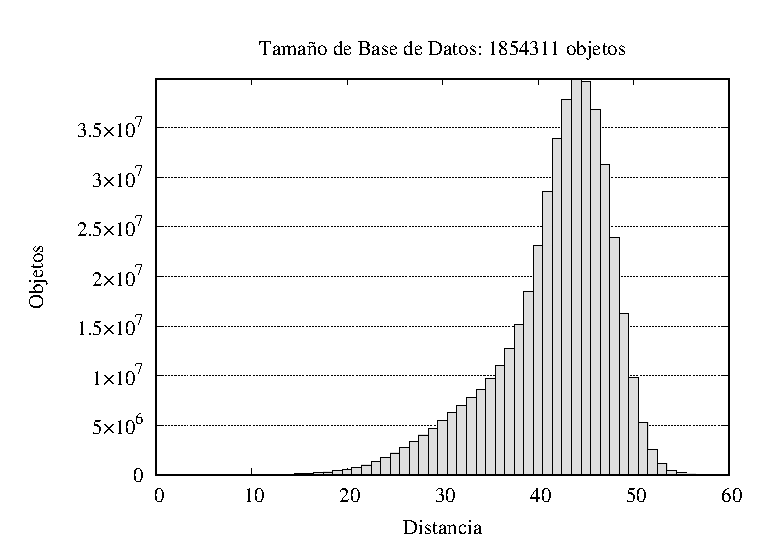
\includegraphics[width=71.5mm]{imagenes/histogramas/1854311_items.eps}}
	\caption{\small Histogramas de frecuencia de la base de datos m\'as grandes del grupo 3 (izquierda) y del grupo 4 (derecha).}
		\label{fig:HF2}
\end{figure} 
\chapter{Conclusiones}

\section{Contribuciones}
 

\appendix
\renewcommand{\appendixname}{Anexos}
\renewcommand{\appendixtocname}{Anexos}
\renewcommand{\appendixpagename}{Anexos}
\addappheadtotoc
\appendixpage

\chapter{T\'ecnicas de selecci\'on de pivotes}\label{anexo.A}
A continuaci\'on incluimos las graficas correspondientes al efecto de las t\'ecnicas de selecci\'on para cada una de las bases de datos que utilizamos.\\

\begin{figure}[h!]
\centering
{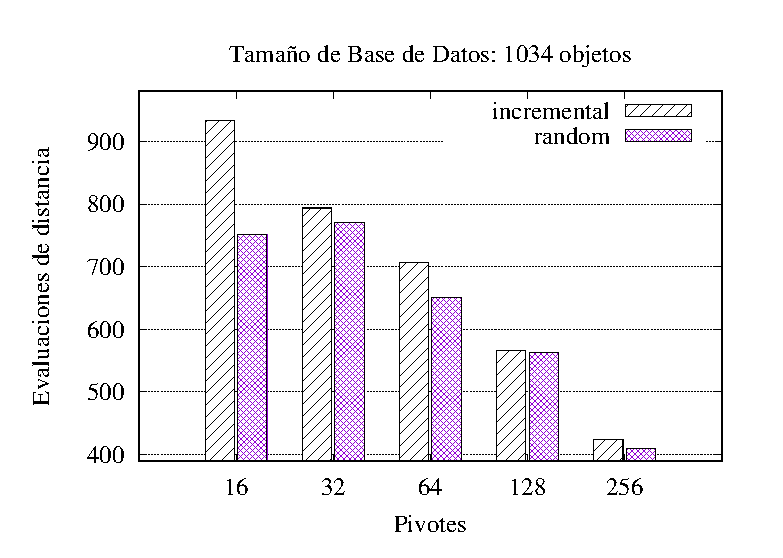
\includegraphics[width=71.5mm]{imagenes/random_vs_incremental/g1_1034.eps}}
{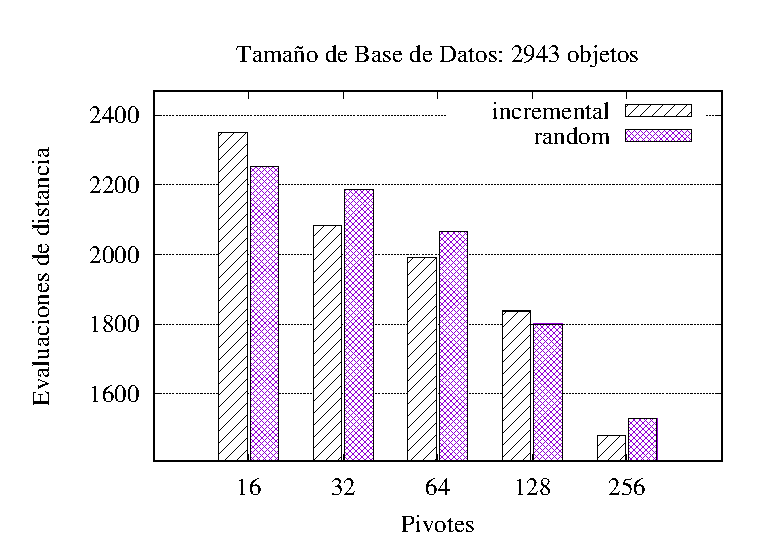
\includegraphics[width=71.5mm]{imagenes/random_vs_incremental/g1_2943.eps}}
{\includegraphics[width=71.5mm]{imagenes/random_vs_incremental/g1_12354.eps}}
{\includegraphics[width=71.5mm]{imagenes/random_vs_incremental/g1_13093.eps}}
\caption{\small Grupo 1 - Efecto de las t\'ecnicas de selecci\'on de pivotes random vs incremental respecto de evaluaciones de distancia.}
\end{figure}

\begin{figure}[h!]
\centering
{\includegraphics[width=71.5mm]{imagenes/random_vs_incremental/g1_15796.eps}}
{\includegraphics[width=71.5mm]{imagenes/random_vs_incremental/g1_15964.eps}}
\caption{\small Grupo 1 - Efecto de las t\'ecnicas de selecci\'on de pivotes random vs incremental respecto de evaluaciones de distancia.}
\end{figure}

\begin{figure}[h!]
\centering
{\includegraphics[width=71.5mm]{imagenes/random_vs_incremental/g2_19032.eps}}
{\includegraphics[width=71.5mm]{imagenes/random_vs_incremental/g2_22421.eps}}
{\includegraphics[width=71.5mm]{imagenes/random_vs_incremental/g2_26903.eps}}
{\includegraphics[width=71.5mm]{imagenes/random_vs_incremental/g2_27788.eps}}
\caption{\small Grupo 2 - Efecto de las t\'ecnicas de selecci\'on de pivotes random vs incremental respecto de evaluaciones de distancia.}
\end{figure}
\begin{figure}[h!]
\centering
{\includegraphics[width=71.5mm]{imagenes/random_vs_incremental/g2_29426.eps}}
{\includegraphics[width=71.5mm]{imagenes/random_vs_incremental/g2_29475.eps}}
{\includegraphics[width=71.5mm]{imagenes/random_vs_incremental/g2_30420.eps}}
{\includegraphics[width=71.5mm]{imagenes/random_vs_incremental/g2_34603.eps}}
{\includegraphics[width=71.5mm]{imagenes/random_vs_incremental/g2_36280.eps}}
{\includegraphics[width=71.5mm]{imagenes/random_vs_incremental/g2_36957.eps}}
{\includegraphics[width=71.5mm]{imagenes/random_vs_incremental/g2_39612.eps}}
{\includegraphics[width=71.5mm]{imagenes/random_vs_incremental/g2_46530.eps}}
\caption{\small Grupo 2 - Efecto de las t\'ecnicas de selecci\'on de pivotes random vs incremental respecto de evaluaciones de distancia.}
\end{figure}


\begin{figure}[h!]
\centering
{\includegraphics[width=71.5mm]{imagenes/random_vs_incremental/g3_57198.eps}}
{\includegraphics[width=71.5mm]{imagenes/random_vs_incremental/g3_77264.eps}}
{\includegraphics[width=71.5mm]{imagenes/random_vs_incremental/g3_77720.eps}}
{\includegraphics[width=71.5mm]{imagenes/random_vs_incremental/g3_86447.eps}}
{\includegraphics[width=71.5mm]{imagenes/random_vs_incremental/g3_87108.eps}}
{\includegraphics[width=71.5mm]{imagenes/random_vs_incremental/g3_93014.eps}}
{\includegraphics[width=71.5mm]{imagenes/random_vs_incremental/g3_106511.eps}}
{\includegraphics[width=71.5mm]{imagenes/random_vs_incremental/g3_136323.eps}}
\caption{\small Grupo 3 - Efecto de las t\'ecnicas de selecci\'on de pivotes random vs incremental respecto de evaluaciones de distancia.}
\end{figure}

\begin{figure}[h!]
\centering
{\includegraphics[width=71.5mm]{imagenes/random_vs_incremental/g4_167995.eps}}
{\includegraphics[width=71.5mm]{imagenes/random_vs_incremental/g4_194687.eps}}
{\includegraphics[width=71.5mm]{imagenes/random_vs_incremental/g4_200375.eps}}
{\includegraphics[width=71.5mm]{imagenes/random_vs_incremental/g4_213578.eps}}
\caption{\small Grupo 4 - Efecto de las t\'ecnicas de selecci\'on de pivotes random vs incremental respecto de evaluaciones de distancia.}
\end{figure}

\chapter{Histogramas de frecuencia}\label{anexo.B}

\begin{figure}[h!]
\centering
{\includegraphics[width=71.5mm]{imagenes/histogramas/1034_items.eps}}
{\includegraphics[width=71.5mm]{imagenes/histogramas/2943_items.eps}}
{\includegraphics[width=71.5mm]{imagenes/histogramas/24708_items.eps}}
{\includegraphics[width=71.5mm]{imagenes/histogramas/26186_items.eps}}
{\includegraphics[width=71.5mm]{imagenes/histogramas/31591_items.eps}}
{\includegraphics[width=71.5mm]{imagenes/histogramas/31928_items.eps}}
\caption{\small Grupo 1 - Histogramas de frecuencia.}
\end{figure}
\begin{figure}[h!]
\centering
{\includegraphics[width=71.5mm]{imagenes/histogramas/38064_items.eps}}
{\includegraphics[width=71.5mm]{imagenes/histogramas/44842_items.eps}}
{\includegraphics[width=71.5mm]{imagenes/histogramas/53806_items.eps}}
{\includegraphics[width=71.5mm]{imagenes/histogramas/55576_items.eps}}
{\includegraphics[width=71.5mm]{imagenes/histogramas/58852_items.eps}}
{\includegraphics[width=71.5mm]{imagenes/histogramas/58949_items.eps}}
\caption{\small Grupo 2 - Histogramas de frecuencia.}
\end{figure}
\begin{figure}[h!]
\centering
{\includegraphics[width=71.5mm]{imagenes/histogramas/60840_items.eps}}
{\includegraphics[width=71.5mm]{imagenes/histogramas/69206_items.eps}}
{\includegraphics[width=71.5mm]{imagenes/histogramas/72560_items.eps}}
{\includegraphics[width=71.5mm]{imagenes/histogramas/73914_items.eps}}
{\includegraphics[width=71.5mm]{imagenes/histogramas/79224_items.eps}}
{\includegraphics[width=71.5mm]{imagenes/histogramas/93060_items.eps}}
\caption{\small Grupo 2 - Histogramas de frecuencia.}
\end{figure}
\begin{figure}[h!]
\centering
{\includegraphics[width=71.5mm]{imagenes/histogramas/114396_items.eps}}
{\includegraphics[width=71.5mm]{imagenes/histogramas/154527_items.eps}}
{\includegraphics[width=71.5mm]{imagenes/histogramas/155440_items.eps}}
{\includegraphics[width=71.5mm]{imagenes/histogramas/172894_items.eps}}
{\includegraphics[width=71.5mm]{imagenes/histogramas/174215_items.eps}}
{\includegraphics[width=71.5mm]{imagenes/histogramas/186027_items.eps}}
{\includegraphics[width=71.5mm]{imagenes/histogramas/213022_items.eps}}
{\includegraphics[width=71.5mm]{imagenes/histogramas/272646_items.eps}}
\caption{\small Grupo 3 - Histogramas de frecuencia.}
\end{figure}
\begin{figure}[h!]
\centering
{\includegraphics[width=71.5mm]{imagenes/histogramas/335989_items.eps}}
{\includegraphics[width=71.5mm]{imagenes/histogramas/389374_items.eps}}
{\includegraphics[width=71.5mm]{imagenes/histogramas/1100749_items.eps}}
{\includegraphics[width=71.5mm]{imagenes/histogramas/1854311_items.eps}}
\caption{\small Grupo 4 - Histogramas de frecuencia.}
\end{figure}
 
\addcontentsline{toc}{chapter}{Referencias}

\bibliographystyle{thesis}
%\bibliographystyle{plain}
\bibliography{bibliografia}


\end{document}